%%
% BIThesis 研究生学位论文模板 The BIThesis Template for Graduate Thesis
% This file has no copyright assigned and is placed in the Public Domain.
% Compile with: xelatex -> biber -> xelatex -> xelatex
%%

% 请勿删除下面两行注释，以免影响编译。
% !TeX program = xelatex
% !BIB program = biber
    
% 为方便您填写内容，模板注释会引用《撰写规范》。该文件是指研函〔2026〕024 号《北京理工大学研究生学位论文撰写规范》，可从以下链接下载。
% https://grd.bit.edu.cn/xwgz/xwgz2/wjxz_xwgz/b117825.htm

\documentclass[type=master,twoside=false,sorting=false]{bithesis}
% 统一三线表线宽，保证首尾横线明显重于中间横线
\setlength{\heavyrulewidth}{1.2pt}
\setlength{\lightrulewidth}{0.7pt}
\setlength{\cmidrulewidth}{0.7pt}
% 硕士论文模板 type=master
% 博士论文模板 type=doctor
% 开启盲审格式 blindPeerReview=true (如：[type=master,blindPeerReview=true])
% 开启双面打印模式 twoside=true (如：[type=master,twoside=true]）
%   《撰写规范》：“论文稿件……双面打印，其中摘要之前部分使用单页打印。”这种效果有以下两种方法实现。
%   - 保持 twoside=false，让打印店帮你操作
%   - 设置 twoside=true，让 LaTeX 自动加若干空白页，然后统一双面打印
%   二者价格差异可忽略不计——校内几家实体打印店（菜市场、国防科技园）都是双面每页￥0.1，很便宜。（截至2024年6月）
%   此外，提交电子版时，一般请保持 twoside=false。
%
% 在 Linux、macOS、Overleaf/TeXPage 等平台，LaTeX 默认使用的中文字体和 Windows 下的字体不同。
% 如果想要获得与 Word 文档相同的效果，请参阅在线帮助 https://bithesis.bitnp.net/faq/word-font.html
%
% 更多使用说明请参考 bithesis.pdf https://mirrors.ctan.org/macros/unicodetex/latex/bithesis/bithesis.pdf

% 以下仅列出常用的配置。全部配置用法请见「bithesis.pdf」手册。
\BITSetup{
  cover = {
    % 使用 date 参数设置封面日期。按《撰写规范》第3页，此处填写论文提交日期、答辩日期或终版论文提交日期，三种均可。
    date = 2026年5月,
    autoWidthPadding = 0.25em,
    % 关闭学生类型勾选框（非工程硕博/交叉/留学生时不需要显示）
    showSpecialTypeBox = false,
  },
  info = {
    % 想要删除某项封面信息，直接删除该项即可。
    % 想要让某项封面信息留空（但是保留下划线），请传入空白符组成的字符串，如"{~}"。
    % 如需要换行，则用 “\\” 符号分割。
    classification = TN929.1,
    UDC = 621.391,
title = 面向复杂水下环境的AFDM无线光通信关键技术研究,
    % 加上下面这一行：
verticalTitle = {面向复杂水下环境的ＡＦＤＭ无线光通信关键技术研究},    % 下面的例子展示了如何在竖排标题中使用垂直或者旋转的英文。
    % verticalTitle = {形状记忆聚氨酯{L } {T } {X }的合成 \rotatebox[origin=c]{-90}{Feng Kaiyu} 及其在纺织中的应用},
    titleEn = {Research on Key Technologies of AFDM-based Wireless Optical Communication in Complex Underwater Environments},
    author = 袁久达,
    authorEn = Yuan Jiuda,
    studentId = 3220230857,
    school = 信息与电子学院,
    schoolEn = School of Information and Electronics,
    supervisor = 郑德智教授,  % 指导教师
    supervisorEn = Prof. Dezhi Zheng,
    chairman = {胡纯教授},  % 答辩委员会主席
    chairmanEn = {Prof. Hui Chun},
    % -------------
    % 请按自身研究生类型填写以下项目
    %
    % --- 学术型 ---
    % degreeType = academic,
    % degree = 工学博士,  % 申请学位
    % degreeEn = Doctor of Engineering,
    % major = 材料科学与工程,  % 一级学科
    % majorEn = Materials Science and Engineering,
    %
    % --- 专业型 --- 
    degreeType = professional, 
    industrialMentor = {王永合},  % 行业合作导师
    industrialMentorEn = {Yonghe Wang},
    degree = 电子信息硕士,  % 申请类别
    degreeEn = {Master of Electronic Information},
    major = 电子信息,  % 学位领域
    majorEn = Electronic Information,
    % -------------
    %
    % 如果想要手动控制盲审模式下的隐藏信息，可以使用宏 \SecretInfo{}。使用方式有两种，如：
    % major = \SecretInfo{材料科学与工程} 可以得到 ******* （用等量的替换符号替代）
    % major = \SecretInfo{材料科学与工程}[ABCDEF] 可以得到 ABCDEF （用你自定义的内容替代）
    %
    submissionDate = 2026年5月,
    submissionDateEn = {May, 2026},
    keywords = {水下无线光通信；仿射频分复用；非对称限幅光仿射频分复用；相干接收；索引调制},
    keywordsEn = {underwater wireless optical communication; affine frequency division multiplexing; asymmetrically clipped optical affine frequency division multiplexing; coherent detection; index modulation},
    %
    % 特别类型——工程硕博士专项
    % 工程硕博士专项 = true,
    % 特别类型——交叉研究方向（一般不用勾选）
    % crossResearch = true,
    % 特别类型——政府项目留学生（一般不用勾选）
    % internationalStudentUGP = true,
    %
    % 必要时置于封面右上角，并按照国家规定进行标记（一般不用标记）
    % classifiedLevel = 密级\BigStar 保密期限,
  },
  % 在目录页中不显示摘要和主要符号对照表的标题。
  TOC = {
    abstract = false,
    abstractEn = false,
    symbols = false,
  },
  style = {
    pageVerticalAlign = top,
    % 开启 Windows 平台下的中易宋体伪粗体。
    % windowsSimSunFakeBold = true,
    % 开启该选项后，将用 Times New Roman 的开源字体 TeX Gyre Termes 作为正文字体。
    % 这个选项适用于以下情况：
    % 1. 不想在系统中安装 Times New Roman。
    % 2. 在 Linux/macOS 下遇到 `\textsc` 无法正常显示的问题。
    % betterTimesNewRoman = true,
  },
  publications = {
    % 以下两个选项将影响「攻读学位期间发表论文与研究成果清单」中名称列表的省略阈值。
    % 一般来说，如果你在全部文献中最低排在第四位，建议你将两个值都设置为大于等于 4 的值。
    % 更详细的说明请见手册。
    maxbibnames = 10,
    minbibnames = 10,
    % 「攻读学位期间发表论文与研究成果清单」默认按学校要求，“按发表的时间顺序列出”。
    % 如需调整，可修改以下选项，详见 https://bithesis.bitnp.net/faq/bib-sort.html
    % sorting = false
  },
  % 采用章节标题级别的附录格式
  appendices / chapterLevel = true,
  misc = {
    % 关闭后，链接会用多种颜色表示，便于检查。
    % 无论是否开启，都不会影响打印效果。
    hideLinks = true,
    % 微调表格行间距
    tabularRowSeparation = 1.6,
  },
}

% 配置参考文献样式
% 现行国标为 GB/T 7714—2015，但其 2025 版将从 2026-07-01 起实施；2026年3月，研究生院老师表示按两版国标均可。
% 以下主要按 2015 版配置，但 gbnamefmt 更接近 2025 版。
% 如果课题组或盲审老师另有特殊要求，您也可修改配置。详情请参考 biblatex-gb7714-2015 的 PDF 文档。
% https://www.ctan.org/pkg/biblatex-gb7714-2015
\usepackage[
  backend=biber,
  style=gb7714-2015,
  sorting=none,
  sortcites=false,
  gbalign=gb7714-2015,
  gbnamefmt=lowercase,
  gbpub=false,
  gbannote=true,
  gbpunctin=false,
  doi=false,
  url=false,
  eprint=false,
  isbn=false,
]{biblatex}

% 强制按引用顺序编号
\ExecuteBibliographyOptions{sorting=none}

\DeclareSourcemap{
  \maps[datatype=bibtex]{
    \map{
      \step[fieldsource=journal, match=\regexp{^Journal of Lightwave Technology$}, replace={J. Lightw. Technol.}]
      \step[fieldsource=journal, match=\regexp{^Electronics Letters$}, replace={Electron. Lett.}]
      \step[fieldsource=journal, match=\regexp{^IEEE Transactions on Wireless Communications$}, replace={IEEE Trans. Wireless Commun.}]
      \step[fieldsource=journal, match=\regexp{^IEEE Wireless Communications Letters$}, replace={IEEE Wireless Commun. Lett.}]
      \step[fieldsource=journal, match=\regexp{^IEEE Communications Letters$}, replace={IEEE Commun. Lett.}]
      \step[fieldsource=journal, match=\regexp{^IEEE Journal on Selected Areas in Communications$}, replace={IEEE J. Sel. Areas Commun.}]
      \step[fieldsource=journal, match=\regexp{^IEEE Transactions on Communications$}, replace={IEEE Trans. Commun.}]
      \step[fieldsource=journal, match=\regexp{^IEEE Transactions on Signal Processing$}, replace={IEEE Trans. Signal Process.}]
      \step[fieldsource=journal, match=\regexp{^Optics Communications$}, replace={Opt. Commun.}]
      \step[fieldsource=journal, match=\regexp{^Optics Express$}, replace={Opt. Express}]
    }
  }
}

% 添加参考文献
\addbibresource{reference/mybib.bib}
\nocite{*}  % 显示 bib 文件中的全部文献条目，包括未在正文中显式引用的


\usepackage{graphicx}

\tracinglostchars=0

% 修正页眉线粗度与页码字体以符合学校撰写规范表2要求
\AtBeginDocument{%
  \renewcommand{\headrulewidth}{0.5pt}%  学校要求0.5磅
  \fancyfoot[C]{\zihao{-5}\rmfamily \thepage}%  Times New Roman 小五号页码
}

\begin{document}

%%%%%%%%%%%%%%%%%%%%%%%%%%%%%%
% 前置部分

\MakeCover % 封面
\MakePaperBack % 书脊
\MakeTitle % 中英文题名页

% 论文原创性声明和使用授权：盲审结束前无需改动
\MakeOriginality
% 后续添加签名时，可考虑先用 Word 制作再导出到 misc/originality.pdf，
% 同时注释以上`\MakeOriginality`，解除注释以下几行代码。
% \begin{blindPeerReview}
%   \cleardoublepage
%   \includepdf[pages=-]{misc/originality.pdf}\newpage
%   % 以上“pages=-”表示插入所有页面。如果你开启了 twoside 双面打印模式，可修改这一参数，例如依次插入第一页、空白页、第二页、空白页：
%   % \includepdf[pages={1, {}, 2, {}}]{misc/originality.pdf}\newpage
% \end{blindPeerReview}

%%
% BIThesis 研究生学位论文模板 The BIThesis Template for Graduate Thesis
% This file has no copyright assigned and is placed in the Public Domain.
%%

% 2026年《撰写规范》更改了致谢页的位置、样式和内容要求，所以这部分会和你的师兄师姐不同。
\begin{acknowledgements}
  三年硕士生涯就这样美好而短暂的过去了，在毕业这个人生节点上，我有太多的话想说。

首先，我要向我的导师郑德智教授致以感谢。感谢郑老师同意我进入这个优秀的课题组。能在团队中度过这段充实的时光，是我的荣幸。

其次，我要将深切的感激之情献给毛天奇老师。在我的整个硕士期间，毛老师是引领我跨越科研河流的领路人。毛老师对我倾注了极大的心血与耐心。是毛老师对学生极其负责的态度、启发性的指导和亦师亦友的人文关怀让我的硕士生涯充满意义。这份恩情我将永远铭记。

此外，我要特别感谢刘光耀师兄。感谢师兄在日常科研中对我不厌其烦的答疑解惑，无论是理论推导的细节还是科研思路的拨正，师兄让我的科研之路少走了许多弯路。

感谢远方的父亲和姐姐，无论我走到哪里，你们始终是我最坚实、最温暖的后盾。感谢你们的默默付出与牵挂，让我能够心无旁骛地追求自己的理想。感谢我的母亲，您始终是我最深的心灵寄托，我很想您。

二十六岁的这一年，站在从校园走向真实世界的十字路口，我还想感谢我自己。感谢考研时埋头努力敢想敢干的你，我没有辜负你的想象，我做的很好。感谢懂得反馈家人的你，我没有遗憾。感谢懂得未雨绸缪的你，我的每一步都走得很踏实。感谢总是想要变得更好的你，我的生活越来越精彩。

未来的路是怎样我也不清楚，但我坚信你什么事情都会做的很好，你也一定能得到你想要的东西，保护好身边的人，勇敢地乘风破浪吧
\end{acknowledgements}
 % 致谢

\frontmatter % 前置部分有两种页面样式，从此切换到第二种

%%
% BIThesis 研究生学位论文模板 The BIThesis Template for Graduate Thesis
% This file has no copyright assigned and is placed in the Public Domain.
%%

\begin{abstract}
  为满足海洋信息网络和空天地海一体化体系中日益增长的水下信息传输需求，本文围绕水下无线光通信在低动态浑浊多径场景和高动态移动场景中的可靠传输问题开展研究。针对不同传播条件下主导失真机制差异显著、传统正交频分复用方案适应性不足的问题，本文以仿射频分复用为统一技术主线，对波形构造、参数设计和检测方法进行了系统研究。本文主要工作与结果如下：

  （1）针对低动态浑浊多径场景中传统光正交频分复用在非负实信号约束下对时延扩展和频率选择性衰落适应性不足的问题，提出面向强度调制直接检测架构的非对称限幅光仿射频分复用方案。该方案改善了传统方案对多径传播和深衰落位置的敏感性，提升了误码率性能与多径鲁棒性；仿真结果表明，在双径条件下相较非对称限幅光正交频分复用约获得 2 分贝增益，在路径数由 2 增至 10 时性能退化更缓。

  （2）针对高动态移动场景中多普勒扩展和相位噪声共同作用下传统方案频偏失配严重的问题，提出面向相干接收的仿射频分复用索引调制方案，并利用静默位置构造残余频偏补偿方法。该方法改善了高动态条件下主导频偏难以低开销补偿的问题，提升了系统在多普勒扩展和激光器线宽扰动下的检测可靠性；仿真结果表明，所提方案在归一化多普勒频移 0 至 0.20 的范围内保持可靠通信，并在高动态条件下优于传统索引调制方案。

  （3）与传统显式导频补偿方案相比，所提方法无需额外导频开销，改善了有效频谱利用率和能量分配效率，避免了 20\% 导频占用带来的约 0.97 分贝等效信噪比损失。
  总体而言，本文形成了面向低动态与高动态两类典型场景的统一设计主线，可为高可靠水下光通信系统设计提供理论参考。 
\end{abstract}

% 如需手动控制换行连字符位置，可写 aa\-bb，详见
% https://bithesis.bitnp.net/faq/hyphen.html

\begin{abstractEn}
  To meet the growing demand for underwater information transmission in marine information networks and integrated space-air-ground-sea systems, this thesis studies reliable transmission for low-dynamic turbid multipath scenarios and high-dynamic mobile scenarios in underwater optical communication. To address the limited adaptability of conventional orthogonal frequency division multiplexing under different dominant impairments, affine frequency division multiplexing is adopted as the unified technical line, and waveform construction, parameter design, and detection methods are investigated systematically. The main improvements and conclusions are as follows:

  (1) For low-dynamic turbid multipath scenarios, an asymmetrically clipped optical affine frequency division multiplexing scheme is proposed for intensity-modulation direct-detection links. The proposed scheme reduces the sensitivity of conventional optical orthogonal frequency division multiplexing to delay spread, frequency-selective fading, and the nonnegative real-signal constraint, thereby improving bit-error-rate performance and multipath robustness. Simulation results show a gain of about 2 decibels over asymmetrically clipped optical orthogonal frequency division multiplexing under the two-path condition, with slower performance degradation when the number of paths increases from 2 to 10.

  (2) For high-dynamic mobile scenarios, a coherent transmission scheme based on affine frequency division multiplexing and index modulation is proposed, together with a residual carrier-frequency-offset compensation method constructed from silent positions. The proposed method alleviates severe frequency-offset mismatch under joint Doppler spread and phase-noise disturbances, and improves detection reliability under Doppler variation and laser-linewidth perturbations. Simulation results show reliable communication over normalized Doppler shifts from 0 to 0.20, while achieving better performance than the conventional index-modulation benchmark in high-dynamic conditions.

  (3) Compared with the conventional pilot-assisted compensation strategy, the proposed method requires no additional pilot overhead, improves effective spectral utilization and power allocation efficiency, and avoids the equivalent signal-to-noise-ratio loss of about 0.97 decibels caused by 20\% pilot occupation. Overall, this thesis establishes a unified scenario-oriented design route for representative low-dynamic and high-dynamic underwater links, and provides theoretical support for reliable underwater optical communication system design.
\end{abstractEn}
 % 摘要

\MakeTOC % 目次
\listoffigures % 插图清单
\listoftables % 附表清单
%%
% BIThesis 研究生学位论文模板 The BIThesis Template for Graduate Thesis
% This file has no copyright assigned and is placed in the Public Domain.
%%

\begin{symbols}
  \item[UWOC] 水下无线光通信（Underwater Wireless Optical Communication）
  \item[AFDM] 仿射频分复用（Affine Frequency Division Multiplexing）
  \item[DAFT] 离散仿射傅里叶变换（Discrete Affine Fourier Transform）
  \item[OFDM] 正交频分复用（Orthogonal Frequency Division Multiplexing）
  \item[IM/DD] 强度调制/直接检测（Intensity Modulation/Direct Detection）
  \item[ACO-AFDM] 非对称限幅光仿射频分复用（Asymmetrically Clipped Optical Affine Frequency Division Multiplexing）
  \item[AFDM-IM] 仿射频分复用索引调制（Affine Frequency Division Multiplexing with Index Modulation）
  \item[$N$] 单个 AFDM/OFDM 符号的总维度或总子载波数
  \item[$G$] 索引调制中的子块数量
  \item[$n$] 单个子块长度，通常满足 $n=N/G$
  \item[$k$] 每个子块中的激活位置数
  \item[$M$] 星座调制阶数
  \item[$c_1$, $c_2$] AFDM/DAFT 变换中的啁啾参数
  \item[$\mathbf{H}_{\mathrm{eq}}$] DAFT 域等效信道矩阵
  \item[$h_p$] 第 $p$ 条传播路径的复增益
  \item[$l_p$] 第 $p$ 条传播路径的离散时延
  \item[$\alpha_p$] 第 $p$ 条传播路径的归一化多普勒频移
  \item[$\phi\lbrack q\rbrack$] 第 $q$ 个离散时刻的相位噪声
  \item[$\Delta\nu$] 相干系统发射端与本振激光器的组合线宽
  \item[BER] 误码率（Bit Error Rate）
\end{symbols}
 % 主要符号对照表

%%%%%%%%%%%%%%%%%%%%%%%%%%%%%%
% 正文部分

\mainmatter

% 请根据论文内容，按照顺序添加章节。
\chapter{绪论}
\label{chap:intro}

\section{研究背景与意义}
\label{sec:background}

随着海洋资源开发、海洋环境观测、水下装备协同作业以及海洋信息网络建设的持续推进，海洋空间中的信息获取、传输与共享需求不断增长。相比陆地通信系统，海洋环境具有传播介质复杂、节点分布分散、部署维护困难以及实时交互要求不断提升等特点，尤其在水下空间，稳定高效的信息链路仍然是制约海洋感知、控制与协同能力提升的关键环节。对于无人潜航器、水下传感器网络、海底作业平台以及移动观测节点而言，若缺乏可靠的高速传输手段，则状态信息、控制指令与大容量感知数据难以及时交换，进而影响整个系统的实时性、协同性和任务执行效率。因此，面向未来海洋信息网络乃至空天地海一体化网络的建设需求，研究适用于不同水下传播条件的高可靠通信技术具有重要的理论意义和应用价值\cite{ShuiXiaWuRenQianHangQiJiQunFaZhanXianZhuangJiGuanJianJiShuZongShuZhongGuoZhiWang, hoeherUnderwaterOpticalWireless2021}。

在多种水下通信手段中，传统水声通信（Underwater Acoustic Communication，UAC）虽然具有传播距离远、技术基础较成熟等优势，但其可用带宽有限、传播时延较大，难以满足高速数据回传、低时延控制与大容量信息交互等需求\cite{liRecentProgressUnderwater2025, jungControlRealTimeMonitoring2025}。同时，射频（Radio Frequency，RF）信号在海水中的传播会受到显著衰减，通常只适用于极短距离或特殊浅水场景，难以支撑常规中远距离高速水下传输\cite{wangEvolutionShortRangeOptical2023}。相比之下，水下无线光通信（Underwater Wireless Optical Communication，UWOC）依托蓝绿光窗口在海水中的相对低衰减特性，具有高带宽、低时延和低截获概率等优势，可作为水下网络中的近距离高速链路、高容量补充链路或局部专用链路，为水下节点间宽带互联提供新的实现路径\cite{kaushalUnderwaterOpticalWireless2016a, departmentofphysicsfacultyofscienceskingabdulazizuniversityjeddah-21589kingdomofsaudiarabiaUnderwaterOpticalCommunications2021a}。已有研究表明，随着 AUV/UUV 集群协同、实时视频回传、近海设施巡检和局部高密度感知任务的发展，水下链路的评价指标已经不再局限于能否连通，而是进一步转向吞吐率、链路恢复速度、控制回路时延与平台机动条件下的可维持性\cite{hoeherUnderwaterOpticalWireless2021, liRecentProgressUnderwater2025, jungControlRealTimeMonitoring2025}。这意味着仅依赖单一载波体制或单一接收架构，往往难以同时覆盖低动态和高动态两类具有代表性的水下应用环境。

需要指出的是，UWOC 的优势并不意味着其传播环境简单。光波在水中传播时会同时受到吸收、散射、湍流、气泡扰动、环境光噪声以及平台姿态变化的影响，不同机理在不同水体类型、链路距离和收发结构下的主导程度并不相同\cite{kaushalUnderwaterOpticalWireless2016a, zengSurveyUnderwaterOptical2017, zayed2026comprehensive}。从系统设计角度看，真正困难的部分并不是单纯追求更高标称速率，而是在复杂损伤机制下构建与场景特征匹配的调制、检测和补偿方法。若忽略主导失真机制随场景变化而切换的事实，就容易把问题抽象得过于理想化，进而削弱方案的物理针对性。

就本文关注的代表性场景而言，UWOC 的关键挑战主要可归纳为两类。第一类是低动态浑浊多径场景。在此类环境中，尽管收发平台相对运动较弱，但悬浮颗粒引起的吸收与散射不仅会造成光功率衰减，还会形成多重散射传播和非视距分量，从而带来明显的时延扩展和频率选择性衰落。第二类是高动态移动场景。在平台高速机动、姿态持续变化或相对速度波动明显的条件下，链路除了面临多径传播外，还会受到多普勒频移、动态指向偏差以及相干接收架构中相位噪声等因素的共同影响，导致系统传输与检测难度显著增加\cite{zengSurveyUnderwaterOptical2017, hamdullahModelingOptimizationNLOS2026, jaruwatanadilokUnderwaterWirelessOptical2008, zhuDopplerResistantOrthogonalChirp2022}。这种场景分化并不是为了方便叙述而人为划分，而是直接对应了物理层设计中“以多径为主”与“以多普勒和相位扰动为主”两条不同的问题链。

针对上述两类典型场景，传统正交频分复用（Orthogonal Frequency Division Multiplexing，OFDM）及其光学扩展形式虽然具有较成熟的实现基础，但也存在明显局限。在低动态多径场景中，传统光 OFDM 体制对傅里叶域正交结构的依赖使其对频率选择性衰落较为敏感；在高动态场景中，多普勒扩展会破坏子载波间的正交关系并引入明显的载波间干扰（Inter-Carrier Interference，ICI），从而削弱 OFDM 借助子载波正交性实现低复杂度频域单抽头均衡的既有优势。对于强度调制/直接检测（Intensity Modulation/Direct Detection，IM-DD）架构而言，系统还需满足发射信号实值非负的物理约束；对于相干接收架构而言，则需进一步处理复数域调制、多普勒扩展与相位噪声共同作用下的复杂检测问题\cite{armstrongOFDMOpticalCommunications2009, yangAdvancementsUnderwaterOptical2024, wolf2024review}。因此，仅依赖传统 OFDM 框架进行局部修正，往往难以同时兼顾不同 UWOC 典型场景下的传播机理与系统约束。

近年来，仿射频分复用（Affine Frequency Division Multiplexing，AFDM）作为一种基于离散仿射傅里叶变换（Discrete Affine Fourier Transform，DAFT）的新型多载波波形，为复杂时延--多普勒耦合信道下的通信提供了新的思路。相关研究表明，AFDM 可通过啁啾参数设计改变信号在变换域中的耦合结构，使时延扩展与多普勒扩展在等效表示域中呈现更具规律性的形式，从而在双选择性信道中表现出较好的适应能力\cite{bemaniAFDMFullDiversity2021, bemani2023affine_nextgen, yin2025affine_extending}。与只在频域上建立正交关系的传统 OFDM 不同，AFDM 更强调对时延和多普勒双重扩展的联合表征，其优势并不局限于高移动射频场景，也体现在复杂传播结构下的参数可调性和表示灵活性\cite{bemani2023affine_thesis, li2025affine_6g, rou2026affine_6g}。对本文研究的两类 UWOC 场景而言，AFDM 的价值并不在于简单替代 OFDM，而在于能够围绕不同场景中的主导失真机制进行有针对性的适配：在低动态浑浊多径场景中增强系统对多径扩展的适应能力，在高动态移动场景中提升系统对多普勒扩展和相位扰动的鲁棒性。这为本文建立统一而清晰的技术主线提供了基础。

在明确了两类场景的主导失真机制与 AFDM 的适配潜力之后，还需要进一步说明本文为何在两类场景中分别采用不同的光接收架构——即低动态场景采用 IM-DD 架构，而高动态场景采用相干接收架构。这一选择并非任意搭配，而是由不同场景下的物理需求所决定的。对于低动态浑浊多径场景，系统设计重点在于应对散射主导的时延扩展，而非载波相位恢复；此时 IM-DD 架构以其实现简单、成本较低的优势，能够满足非相干场景下的基本检测需求，且无需引入本振激光器和复杂的相位同步机制，因而是工程上更为经济的选择。然而，IM-DD 架构仅利用光强维度，在物理上无法恢复接收信号的相位信息，这意味着它无法支撑复数域 AFDM 调制所需的幅度--相位联合检测，也无法执行依赖相位结构的多普勒补偿操作。当场景转向高动态条件时，多普勒频偏的存在要求接收端必须能够观测并补偿载波相位的线性斜坡，同时高阶复数调制对接收灵敏度的要求也更为严格；此时相干接收架构通过引入本振激光器进行零差或外差混频，能够完整恢复信号的幅度与相位信息，从而为后续的复数域信号处理、多普勒补偿以及高阶调制检测提供物理前提\cite{guiomarCoherentFreeSpaceOptical2022, huPerformanceCoherentOptical2025}。此外，相干架构在接收灵敏度方面通常优于直接检测方案，这对于高动态条件下因指向偏差和链路不稳定导致接收光功率波动的场景尤为重要。因此，本文从低动态到高动态的架构切换，本质上是围绕不同场景下物理层对信号维度的利用需求所做的系统性选择：低动态场景仅需强度维度即可满足设计目标，高动态场景则必须借助相位维度才能完成多普勒补偿与高灵敏度检测。

基于上述认识，本文围绕 UWOC 场景下的 AFDM 波形设计与检测方法展开研究。针对低动态浑浊多径场景，结合 IM-DD 架构的物理约束，提出一种非对称限幅光仿射频分复用（Asymmetrically Clipped Optical Affine Frequency Division Multiplexing，ACO-AFDM）传输方案，以提高系统在非负实信号约束下对频率选择性衰落的适应能力；针对高动态移动场景，结合相干接收与索引调制（Index Modulation，IM；注：此处 IM 指索引调制，与前述 IM-DD 中的强度调制含义不同）机制，提出一种相干 AFDM-IM 传输方案，以提升系统在多普勒扩展和相位噪声共同作用下的传输可靠性。两类方案虽然面向不同场景，但均以 AFDM 为统一技术主线，体现了本文围绕典型 UWOC 传播条件进行波形适配与检测设计的总体思路。

本文工作的价值主要体现在以下几个方面。第一，从理论层面，本文围绕水下光信道中的多径、多普勒及相位噪声等代表性失真机制，分析 AFDM 在不同动态条件下的适配方式，拓展了其在 UWOC 场景中的应用研究。第二，从方法层面，本文针对 IM-DD 与相干接收两种不同架构，分别构建 ACO-AFDM 与相干 AFDM-IM 两类方案，体现了同一技术主线在不同物理约束下的系统化设计思路。第三，从应用层面，本文研究可为未来近距离高速水下链路、局部高容量水下组网以及移动平台协同通信等场景提供一定的理论参考。

\section{国内外研究现状}
\label{sec:research_status}

围绕 UWOC 的可靠传输问题，国内外研究已从早期的链路可行性验证逐步发展到对传播环境、接收架构、波形设计与检测算法的系统研究。总体而言，现有工作主要涉及水下光信道建模、面向多径失真的调制与检测方法、新型抗时延--多普勒波形设计，以及高动态场景下的相干传输与索引调制等方向。结合本文的研究主线，现有研究可概括为以下三个方面。

\subsection{水下光信道及低动态多径场景相关研究}
\label{subsec:status_modulation}

准确描述水下光传播过程是开展 UWOC 系统设计的基础。Kaushal 等对水下无线光通信的关键问题进行了系统总结，指出不同海域类型下的吸收、散射与链路损耗差异会直接影响传输距离、链路稳定性和系统设计方式\cite{kaushalUnderwaterOpticalWireless2016a}。Zeng 等系统梳理了 UWOC 中吸收、散射、湍流与链路建模等问题，进一步说明了水下光通信在短距高速传输中的应用潜力\cite{zengSurveyUnderwaterOptical2017}。Jaruwatanadilok 基于矢量辐射传输理论分析了水下光传播特性，指出多重散射会导致明显的时延扩展，并在高速传输条件下引发频率选择性衰落与符号间干扰（Inter-Symbol Interference，ISI）\cite{jaruwatanadilokUnderwaterWirelessOptical2008}。这些研究表明，即使在低动态平台条件下，浑浊水体中的多径传播仍可能成为限制系统性能的重要因素。

近年的研究进一步把这一认识从定性描述推进到更细致的建模层面。Ramley 等从蒙特卡罗方法出发，对 UWOC 信道仿真的主要路线进行了综述，指出辐射传输方程求解、光子轨迹统计与脉冲响应重构之间具有紧密联系，水下光信道建模已经从简单衰减近似逐步转向面向系统设计的端到端表征\cite{ramley2024overview}。Chen 等给出了非视距水下激光链路的冲激响应分析方法，说明前向散射与后向散射会共同改变 CIR 的形状，进而影响高速传输中的符号间干扰分布\cite{chen2022modeling}。Zayed 等则从吸收、散射、湍流、指向误差、环境光与接收噪声等多个维度总结了 UWOC 端到端建模中的主要损伤项，强调面向系统优化的信道建模不应只关注单一衰减系数，而应同时考虑随机衰落和几何失准等效应\cite{zayed2026comprehensive}。

除了平均衰减，多重散射和随机介质扰动还会显著改变接收信号的统计特性。Majlesein 等研究了水下散射噪声随水质和传输距离变化的趋势，指出经历散射的光子比例增加时，链路带宽和误码性能都会受到影响\cite{majlesein2021investigation}。Kou 等建立了包含多尺寸颗粒、气泡和湍流效应的复合衰落模型，并给出了多重散射对接收功率、冲激响应扩展和体积散射函数的影响规律\cite{kou2023composite, kou2025investigation}。Ata 等从弱湍流到中强湍流的不同统计模型出发，推导了 IM-DD 体制下 BER 的闭式表达式，表明水体参数变化会直接映射到接收性能退化程度\cite{ata2023analysis}。这些结果说明，所谓“低动态”仅意味着平台运动相对较缓，并不意味着传播信道可以被近似为平坦、稳定且易于均衡的理想链路。

为减弱频率选择性衰落对系统性能的影响，OFDM 技术被引入光通信领域。Armstrong 系统阐述了光 OFDM 的基本原理及其在光链路中的适用性\cite{armstrongOFDMOpticalCommunications2009}。在 IM-DD 架构下，为满足发射信号非负实值约束，直流偏置光 OFDM（Direct Current Biased Optical OFDM，DCO-OFDM）与非对称限幅光 OFDM（Asymmetrically Clipped Optical OFDM，ACO-OFDM）得到了广泛研究。Dissanayake 等对 ACO-OFDM 与 DCO-OFDM 进行了对比分析，指出 ACO-OFDM 能够将限幅噪声限制在偶数子载波，从而保证奇数子载波上的有效信息恢复\cite{dissanayakeComparisonACOOFDMDCOOFDM2013}。Essalih 等进一步表明，在相同频谱效率条件下，ACO-OFDM 具有较好的光功率效率\cite{essalihOpticalOFDMSiPMBased2020}。Fernando 等提出 U-OFDM 等单极性光多载波方案，也从不同角度拓展了 IM-DD 系统中 OFDM 的实现方式\cite{fernandoFlipOFDMUnipolarCommunication2011}。Wolf 等对带限 IM/DD 光系统中的先进调制格式进行了综述，指出非负约束、带宽限制与器件动态范围往往需要联合考虑，而不是将多载波设计与光电前端分离处理\cite{wolf2024review}。此外，Jihad 等在其他光无线场景中展示了 ACO 类结构在受限光强发射条件下的可行性，也说明限幅型单极性 OFDM 仍然具有持续的结构研究价值\cite{jihad2021twodimensions}。

尽管如此，现有 IM-DD 光 OFDM 方案总体上仍建立在傅里叶域正交结构基础上，当水下多径扩展较为显著时，系统对深度频率选择性衰落仍较为敏感。Yang 等针对 UWOC 中 OFDM 的仿真研究也表明，信道建模精度、PAPR 控制与接收端鲁棒性会显著影响系统实际收益\cite{yangAdvancementsUnderwaterOptical2024}。Sarkar 等在清洁海水条件下对 OFDM 型 UWOC 系统的性能分析表明，即便在较理想的介质条件下，多径和散射仍会约束高阶调制增益的释放\cite{sarkar2025performance}。因此，面向低动态浑浊多径场景，仍有必要探索兼顾 IM-DD 约束与多径鲁棒性的改进波形设计。本文第三章所研究的 ACO-AFDM 方案，正是在这一背景下对传统光 OFDM 思路的进一步拓展。

\subsection{AFDM 及抗时延--多普勒波形研究现状}
\label{subsec:status_doppler}

随着无线通信系统逐步面向更复杂的时变信道环境，传统 OFDM 在时延扩展与多普勒扩展共同作用下的性能瓶颈日益突出。为提高系统对双选择性信道的适应能力，研究重点逐渐从传统傅里叶域多载波体制转向新型时频耦合波形设计。

Bemani 等提出了 AFDM 技术，并指出通过合理配置啁啾参数，可使离散线性时变信道在 DAFT 域中获得更具结构性的表示，从而提升系统对时延与多普勒扩展的适应能力\cite{bemaniAFDMFullDiversity2021}。与仅在频域上构建正交关系的传统 OFDM 相比，AFDM 能够更自然地表征时延--多普勒耦合信道，为双选择性环境下的信号检测与均衡提供新的实现基础。随后，围绕 AFDM 的研究不断拓展到参数设计、等效信道表示、低复杂度检测与扩展调制机制等方向。Bemani 的博士论文对 AFDM 的理论结构、全分集条件、低复杂度检测以及嵌入式信道估计方案进行了更系统的梳理，为后续研究提供了相对完整的分析框架\cite{bemani2023affine_thesis}。在此基础上，Bemani 等又从下一代无线通信视角进一步论证了 AFDM 在双选择性信道中的最优分集潜力，并给出了更完整的输入输出关系和参数设计依据\cite{bemani2023affine_nextgen}。

AFDM 的研究正在逐步从“新体制提出”走向“结构特性与应用边界细化”。Yin 等指出，AFDM 可以被理解为 OFDM 在更一般场景下的拓展，其可调啁啾参数使系统能够在不同传播条件间实现更强的场景适配能力\cite{yin2025affine_extending}。Li 等和 Rou 等分别从 6G 候选波形和高移动鲁棒性角度综述了 AFDM 的基本性质，强调其作为 chirp-based 多载波波形，在兼顾结构规则性和场景灵活性方面具有潜力\cite{li2025affine_6g, rou2026affine_6g}。Zhou 等进一步把 AFDM 放到通信与信道探测一体化框架下讨论，说明其完整的时延--多普勒表示不仅有利于数据传输，也为动态信道感知提供了额外空间\cite{zhou2025affine_channel}。这些工作共同表明，AFDM 的意义不应被狭义理解为“抗多普勒 OFDM 替代物”，而应被理解为一种更适于处理结构化时变信道的新型变换域建模工具。

从相关体制比较角度看，AFDM 也并非孤立发展。Rou 等对 OTFS 与 AFDM 的比较研究指出，两者都试图在时延--多普勒域中建立更稳定的等效表示，但 AFDM 在多啁啾结构和参数化设计方面呈现出不同于 OTFS 的实现特点\cite{rou2024from_otfs}。Li 等针对宽带双分散信道中的时间尺度效应分析了 AFDM 的输入输出关系，说明当传播机理更复杂时，AFDM 仍可通过参数设计保持离散变换域信道的稀疏结构\cite{li2025affine_wideband}。这些研究扩展了 AFDM 的理论适用范围，也说明其并不是只对单一场景有效的特定技巧，而是具备进一步迁移到光无线、跨介质和高动态链路中的潜力。

AFDM 的潜力并不局限于高动态场景。虽然其最初更多被用于处理双选择性信道，但从更一般的信号处理角度看，只要传播环境中存在可利用的结构化时移或时移--频移耦合特征，AFDM 就有可能比传统傅里叶体制提供更适配的表示方式。对于低动态多径场景，AFDM 可以增强系统对路径时延结构的描述能力；对于高动态场景，AFDM 则更直接体现出对多普勒扩展的适应性。因此，将 AFDM 作为贯穿全文的统一技术主线，不仅有助于连接低动态与高动态两类场景，也有助于构建具有一致理论基础的方案体系。

不过，现有 AFDM 研究多集中于射频双选择性信道或一般复数基带系统，对 IM-DD 光学发射约束、相干光接收架构以及水下光链路传播特点的针对性研究仍较少。Kumar 等将 AFDM 引入水下光网络仿真框架后指出，虽然 AFDM 在动态信道中具有理论优势，但水下环境中的散射、吸收与链路失准会改变其实际收益释放条件\cite{kumar2025optical_network}。Liu 等对实际 DAC/ADC 滤波器影响下的 AFDM 进行了分析，说明硬件前端会改变等效 DAFT 域信道结构，这对工程化实现同样重要\cite{liu2025affine_dac}。因此，如何将 AFDM 与非负光发射结构、相干探测和索引调制机制有机结合，仍有较大的研究空间。本文正是在这一研究空缺下，将 AFDM 分别扩展到低动态 IM-DD 场景和高动态相干场景之中。

\subsection{高动态 UWOC、相干接收与索引调制研究现状}
\label{subsec:status_coherent}

随着 UUV 集群协同、动态平台互联和实时水下感知等应用的发展，UWOC 链路正由低动态、准静态应用逐步向高动态场景拓展\cite{MianXiangUUVJiQunYingYongDeShuiXiaWuXianGuangTongXinGuanJianJiShu2025}。在此类条件下，平台相对运动引起的多普勒频移会破坏传统 OFDM 子载波间的正交关系，导致明显 ICI，并使系统性能迅速下降\cite{zhuDopplerResistantOrthogonalChirp2022, fernandesDigitallyMitigatingDoppler2023}。与此同时，光束发散角有限、平台姿态快速变化和收发对准误差也会使高动态链路比静态链路更容易出现功率波动和瞬时失锁\cite{hoeherUnderwaterOpticalWireless2021, derakhshandehUnderwaterCoherentOptical2025}。因此，面向高动态 UWOC 的抗多普勒传输技术已成为当前研究的重要方向。

除波形鲁棒性外，接收架构也是影响高动态 UWOC 性能的重要因素。尽管 IM-DD 架构具有实现简单的优点，但其在接收灵敏度与复数域调制支持方面存在明显限制。为此，相干光接收逐渐受到关注。Guiomar 等指出，相干接收能够恢复光信号的幅度与相位信息，并结合数字信号处理提升系统性能\cite{guiomarCoherentFreeSpaceOptical2022}。Hu 等的理论分析表明，在复杂光信道条件下，相干探测在接收灵敏度与背景噪声抑制方面优于直接探测\cite{huPerformanceCoherentOptical2025}。Zedini 等进一步比较了不同探测类型在 UWOC 湍流信道中的性能，结果表明异频/相干检测在 BER 和容量方面具有明显优势\cite{zediniEvaluationUnderwaterOptical2025}。然而，相干架构在带来性能增益的同时，也会引入由激光器有限线宽导致的相位噪声问题。Tang 等指出，组合线宽增大会显著削弱水下相干通信性能，因此相关系统设计需要同时考虑多普勒扩展与相位噪声影响\cite{tangUnderwaterCoherentOptical2021}。Du 等对维纳相位噪声方差的最大似然估计研究也表明，相位随机过程并非可以忽略的次要扰动，而是会直接影响后续补偿与检测的估计精度\cite{du2024maximum}。

高动态 UWOC 的另一个特点在于，多普勒、相位噪声与指向误差往往不是相互独立的后处理项，而是与波形结构、接收算法和硬件链路共同耦合。Derakhshandeh 等在自适应光学辅助的水下相干链路研究中指出，电子波束控制、孔径平均和湍流补偿能够在一定程度上延长链路距离，但系统仍需与更合适的传输和检测结构联合设计\cite{derakhshandehUnderwaterCoherentOptical2025}。这说明高动态 UWOC 的难点不仅在于“补一个频偏”，而在于如何在可观测的幅度--相位维度上构建能适应多重损伤的统一接收处理框架。

为进一步提高频谱效率与能量利用效率，索引调制也被引入多载波系统设计。Basar 等较早在 OFDM 中引入索引调制，证明了激活位置可作为附加信息维度承载比特\cite{basarOrthogonalFrequencyDivision2013}。Li 等进一步将索引映射扩展到能量和星座等多域结构，说明索引调制不仅能够提高频谱效率，还可以改变多载波系统的信息承载方式\cite{li2022composite}。随后，Tao 等与 Zhang 等分别提出 AFDM-IM 及相关扩展方案，表明 AFDM 与索引调制的结合可通过稀疏激活结构提高信息承载效率并改善检测性能\cite{taoAffineFrequencyDivision2025, zhangDualIndexModulation2026}。不过，现有 AFDM-IM 研究同样主要集中于射频场景，其在高动态 UWOC 中与相干接收架构相结合的研究仍相对有限。对于水下光链路而言，未激活位置除了可以承载索引信息外，还有可能作为隐式结构参考参与频偏感知和检测过程，这也是本文第四章进一步展开的关键思路。

综合来看，现有研究已分别在水下光信道建模、IM-DD 光 OFDM、AFDM 波形设计以及高动态相干传输等方面取得一定进展，但仍缺乏一条围绕 UWOC 典型场景特征展开的统一研究主线。特别是，如何基于 AFDM 这一新型波形，同时面向低动态浑浊多径场景和高动态移动场景构建有针对性的水下光通信方案，仍有进一步研究空间。这正是本文工作的主要切入点。

\section{本文主要研究内容与章节安排}
\label{sec:research_contents}

本文面向 UWOC 在两类典型场景下的可靠传输需求，围绕 AFDM 波形设计、参数配置与检测方法开展研究，力图建立一条从信道特性分析到场景化传输方案设计的完整技术链路。全文的研究目标不是分别解决两个彼此割裂的小问题，而是以 AFDM 为统一技术主线，探索其在低动态多径场景与高动态时变场景中的适配方式及性能优势。

围绕这一总体目标，本文的主要研究内容包括以下两个方面。

第一，针对低动态浑浊多径 UWOC 场景，研究面向 IM-DD 架构的 ACO-AFDM 传输方案。该部分工作从 IM-DD 系统中发射信号的实值非负约束出发，将 ACO 结构与 AFDM 波形相结合，构建适用于低动态多径传播条件的 ACO-AFDM 系统模型；在此基础上，围绕余弦型 DAFT 核分析参数设计中的奇异点规避和多径分离条件，给出兼顾逆变换稳定性与多径鲁棒性的啁啾参数设计准则；最后通过仿真验证所提方案在低动态多径场景下相对于传统光 OFDM 方案的误码率性能优势和多径适应能力。

第二，针对高动态移动 UWOC 场景，研究面向相干接收的 AFDM-IM 传输方案。该部分工作从高动态条件下多普勒扩展和相位噪声共同作用的特点出发，建立包含多径、多普勒频移与维纳相位噪声的系统模型，并推导 DAFT 域下的等效输入输出关系；进一步利用 AFDM-IM 发送向量中未激活位置所对应的静默结构作为隐式参考，构造基于泄露能量最小化与稀疏度量驱动的盲搜方法，在无额外导频开销下精准补偿主导的残余载波频偏，并对维纳相位噪声实现鲁棒容忍；最后通过仿真分析所提方案在高动态条件和不同激光器线宽下的 BER 性能与鲁棒性。

除上述两项核心工作外，本文还从统一理论基础出发，对水下光传播机理、双选择性信道模型、传统 OFDM 的局限性以及 AFDM 的基本原理进行了系统梳理，使第三章与第四章的场景化方案设计能够建立在一致的分析框架之上。综合而言，本文的研究内容覆盖了从低动态到高动态、从 IM-DD 到相干接收、从波形设计到检测算法的多个层面，但其内在逻辑始终围绕同一主线展开，即：针对 UWOC 不同代表性传播条件下的主导失真机制，对 AFDM 进行有针对性的系统适配与性能验证。

\subsection{章节安排}
\label{subsec:chapter_arrangement}

本文共分为五章，各章内容安排如下。

第一章为绪论，主要介绍论文的研究背景与意义，分析 UWOC 在未来海洋信息网络和近距离高速水下链路中的应用价值，梳理低动态浑浊多径场景与高动态移动场景下的代表性物理层挑战，综述国内外在相关方向上的研究进展，并给出本文的主要研究内容与章节安排。

第二章为水下光通信系统模型与理论基础。该章从水下光传播机理出发，分析吸收、散射和湍流等因素对链路的影响，建立时变双选择性信道的数学模型，讨论传统 OFDM 在时变信道中的局限性，并介绍 AFDM 的基本原理、DAFT 结构及其对本文两类典型场景的支撑作用，为后续章节的方案设计奠定理论基础。

第三章为面向低动态水下场景的 ACO-AFDM 传输方案。该章针对低动态浑浊多径条件下 IM-DD 系统面临的非负实值约束与频率选择性衰落问题，构建 ACO-AFDM 系统模型，研究其参数设计方法，并通过仿真验证方案在误码率性能和多径鲁棒性方面的优势。

第四章为面向高动态水下场景的相干 AFDM-IM 传输方案。该章针对高动态 UWOC 中多径、多普勒扩展和相位噪声共同作用下的传输问题，建立相干 AFDM-IM 系统模型，推导 DAFT 域等效输入输出关系，并利用 AFDM-IM 静默位置作为隐式参考，围绕泄露能量最小化与稀疏度量构造盲搜方法，在无额外导频开销下精准补偿主导的残余载波频偏并对维纳相位噪声实现鲁棒容忍。

第五章为总结与展望。该章对全文工作进行归纳总结，概括本文在低动态 ACO-AFDM 方案和高动态相干 AFDM-IM 方案方面的主要研究结论，分析当前工作的不足，并对 AFDM 在 UWOC 中的后续研究方向进行展望。

通过上述章节安排，全文在结构上形成了问题背景与研究定位—理论基础—低动态方案—高动态方案—总结展望的递进逻辑，从而较为完整地体现出本文围绕 AFDM 在 UWOC 两类典型场景中应用展开研究的主线。

\chapter{水下光通信系统模型与理论基础}
\label{chap:theory_model}

可靠的水下无线光通信系统设计，需要以对水下光学传播机理和信道特性的准确认识为基础。本章围绕水下光学信道特性、时变双选择性信道模型、传统 OFDM 的局限性以及 AFDM 的基本原理展开分析，为后续传输方案设计奠定理论基础。

\section{水下光学信道特性分析}
\label{sec:underwater_channel}

光束在不同类型海水中传播时，会受到水分子、溶解物及悬浮颗粒的共同影响，主要表现为吸收、散射以及光学湍流等效应\cite{kaushalUnderwaterOpticalWireless2016a}。与陆地自由空间光通信相比，水下介质具有更强的吸收与散射特性，且其统计性质会随海域类型、颗粒浓度、温盐分布以及流体扰动状态的变化而明显改变。因此，UWOC 链路的传播损耗、可达距离以及时变特征都与具体水体环境密切相关。

从工程应用角度看，不同海域环境下的水下光链路往往表现出显著不同的传播条件。在清澈海水中，吸收与散射相对较弱，系统可获得更长的有效通信距离；而在近岸海域、港口水域或高浑浊水体中，悬浮颗粒浓度上升会显著增强散射效应，使链路衰减加剧并引入更明显的多径传播。由于本文关注的典型低动态场景往往对应浑浊水体中的短距链路，因此有必要从吸收、散射及其引发的时延扩展出发，对水下光信道的物理机理进行分析。

\subsection{吸收与散射效应}

吸收效应是指光子能量在与水体介质相互作用过程中转化为其他形式能量，从而导致光功率随传播距离增加而衰减。散射效应则是指光子在遇到悬浮颗粒后传播方向发生偏转。散射不仅会降低接收端收集到的有效光功率，还会因多重散射引起传播路径差异，进而造成时延扩展\cite{jaruwatanadilokUnderwaterWirelessOptical2008}。

在 UWOC 系统中，吸收与散射引起的综合衰减通常采用 Beer-Lambert 定律描述。设发射光功率为 $P_t$，传播距离为 $L$，则接收光功率 $P_r$ 可表示为
\begin{equation}
    P_{r} = P_{t} \exp(-c(\lambda) L)
\label{eq:beer_lambert}
\end{equation}
其中，$c(\lambda)$ 为总衰减系数，由吸收系数 $a(\lambda)$ 与散射系数 $b(\lambda)$ 组成，即 $c(\lambda)=a(\lambda)+b(\lambda)$\cite{zengSurveyUnderwaterOptical2017}。式(\ref{eq:beer_lambert}) 表明，在其他条件不变时，接收光功率随传播距离增加呈指数衰减。

需要指出的是，$a(\lambda)$ 与 $b(\lambda)$ 具有明显的波长相关性，因此波长选择会直接影响系统的传播损耗。现有研究表明，蓝绿光波段在海水中通常具有相对较低的总衰减系数，因此常被用作 UWOC 的主要工作窗口。这一波段能够在吸收与散射之间取得相对有利的平衡，使系统在有限发射功率下获得更大的传输距离和更高的接收信噪比。然而，不同水体环境对最优工作波长的影响并不完全一致：当水体浑浊程度提高时，散射增强会缩小系统的有效覆盖范围，并使链路性能对发射光束发散角、接收视场角及收发对准精度更加敏感。

除平均功率衰减外，散射过程还会对信号波形结构产生重要影响。对于非视距分量或多重散射分量，不同光子到达接收端的传播时间往往存在差异，因而会形成离散或连续分布的延迟分量。当信号带宽较高、符号周期较短时，这些延迟分量可能跨越多个采样间隔，从而使接收端观察到明显的时延扩展。时延扩展的直接后果是相邻符号之间发生叠加，并进一步导致频率选择性衰落。对于多载波系统而言，这意味着不同频率位置上的信道响应不再一致，部分子带可能出现深衰落，进而提高均衡与检测难度。

因此，在低动态浑浊水下场景中，影响系统性能的关键并不只是平均光功率损耗，还包括散射所引起的多径传播结构。换言之，即使收发平台相对运动较弱，信道仍可能由于介质本身的散射特性而表现出显著的频率选择性。这也是本文在低动态场景下重点关注多径鲁棒性设计的重要原因。

\subsection{水下光学湍流}

除吸收与散射外，温度梯度、盐度变化及洋流扰动还会导致水体折射率随机波动，形成水下光学湍流。湍流会引起波前畸变与光强闪烁，进而造成接收信噪比波动。在理论建模中，弱湍流条件下常采用对数正态分布描述衰落，中强湍流条件下则可采用 Gamma-Gamma 分布或其他复合统计模型进行表征\cite{zediniEvaluationUnderwaterOptical2025, huPerformanceCoherentOptical2025}。

与大气光通信中的湍流效应类似，水下光学湍流同样会导致接收功率的随机起伏，但其形成机理更容易受到局部温盐分层、流场扰动以及设备运行热源的影响。在短距离 UWOC 链路中，湍流造成的平均衰减未必占主导地位，但其对瞬时信噪比波动、误码性能离散性以及链路稳定性的影响仍不可忽略。当系统采用高阶调制或高灵敏度接收架构时，湍流引起的随机功率波动还可能放大同步误差与信道估计误差对检测性能的影响。

对于高动态场景而言，湍流效应还可能与平台运动造成的动态指向误差共同作用。平台姿态变化、机械振动以及波浪扰动会使收发端光束轴线发生偏移，导致接收面上的能量分布变化。当接收孔径较小或视场角较窄时，这类指向误差会进一步放大链路增益波动。尽管本文在后续模型中主要聚焦多径、多普勒和相位噪声影响，但从物理层角度看，湍流与指向误差仍是影响真实 UWOC 系统稳健性的重要因素，也是未来实验验证与模型拓展中需要进一步考虑的内容。

综上，水下光信道并非单一的功率衰减通道，而是同时包含吸收、散射、湍流及动态指向误差等多种扰动机制的复合信道。对于低动态场景，散射主导的时延扩展是影响系统设计的关键；对于高动态场景，平台运动与器件非理想性带来的时变效应则更加突出。对这些传播特性的分析，为后续建立双选择性信道模型和设计针对性传输方案提供了物理依据。

\section{时变双选择性信道数学模型}
\label{sec:doubly_selective_model}

在高动态 UWOC 场景中，水体散射引起的多径扩展与平台相对运动引起的多普勒扩展共同作用，使信道呈现明显的时变双选择性特征\cite{bemaniAFDMFullDiversity2021}。所谓双选择性，是指信道既在频率维度上表现出选择性衰落，又在时间维度上呈现快速变化特性。前者主要由时延扩展造成，后者主要由多普勒扩展引起。对于面向高速传输的 UWOC 系统，这两类效应往往难以彼此分离处理，因此需要统一的数学模型进行描述。

\subsection{多径与多普勒效应}

设最大时延扩展为 $\tau_{\max}$，最大多普勒频移为 $\nu_{\max}$。当时延扩展相对于符号周期不可忽略时，系统将表现出频率选择性衰落；当多普勒频移导致信道在一个传输帧内发生明显变化时，系统将表现出时间选择性衰落。这两类效应共同作用，会显著增加系统均衡与检测的难度。

从系统分析角度看，时延扩展通常可与相干带宽联系起来理解。若信号带宽超过信道相干带宽，不同频率分量将在传播过程中经历不同幅相响应，系统便会表现出明显的频率选择性。在多载波系统中，这意味着不同子载波所经历的信道增益不再一致，部分子载波甚至可能落入深衰落区。类似地，多普勒扩展通常可与相干时间相关联。当传输帧持续时间接近或超过信道相干时间时，信道在一帧内部便不能再视为准静态，从而使基于固定子载波正交关系或固定均衡系数的设计难以保持有效。

对于 UWOC 而言，低动态场景与高动态场景的主导失真机制并不相同。在低动态浑浊水体中，多径扩展往往更突出，系统的主要困难在于如何抑制时延扩展带来的频率选择性衰落与符号间干扰；而在高速移动场景中，平台相对运动会显著增强多普勒扩展，使时间选择性和载波间耦合问题变得更加突出。当两类效应同时存在时，系统接收端所面对的便不再是单纯的卷积信道，而是一个具有时变耦合结构的双选择性信道。

\subsection{基带等效信道表示}

对于包含 $P$ 条离散路径的水下线性时变信道，其时变基带等效冲激响应可写为
\begin{equation}
    h(t, \tau) = \sum_{i=1}^{P} h_{i} e^{j 2 \pi \nu_{i} t} \delta(\tau - \tau_{i})
\label{eq:ltv_channel}
\end{equation}
其中，$h_i$、$\tau_i$ 与 $\nu_i$ 分别表示第 $i$ 条路径的复增益、传播时延和多普勒频移。在离散时间域中，若采样间隔为 $T_s$、系统维度为 $N$，则该信道可等效表示为一个 $N \times N$ 的时变矩阵。由式(\ref{eq:ltv_channel}) 可见，不同路径同时引入时延与多普勒扩展，因而难以借助传统傅里叶域表示实现有效对角化。

进一步地，若令离散时延为 $l_i=\tau_i/T_s$，归一化多普勒为 $\alpha_i=\nu_i N T_s$，则每一路径均可视为“循环移位 + 相位旋转”的组合操作。于是，整个信道可以看作多个时移--频移算子的叠加。对于仅包含时延扩展而无明显多普勒扩展的情况，信道矩阵近似为循环卷积结构，较易通过 OFDM 等体制实现对角化处理；但当多普勒项不可忽略时，信道矩阵将由近似对角形式演化为具有带状耦合特征的时变矩阵，子载波之间会出现明显的能量泄露与相互干扰。

从连续模型过渡到离散模型的意义在于，后续系统设计和算法推导通常都以离散基带信号为研究对象。通过将信道表示为有限维矩阵形式，可以更方便地讨论不同波形在等效变换域中的结构特征，并据此构造检测与均衡方法。特别是对于本文关注的 AFDM 体制，信道在合适变换域中的耦合结构将直接决定后续参数设计和检测算法的复杂度。

\subsection{双选择性信道对系统设计的影响}

双选择性信道对通信系统设计的影响主要体现在三个方面。其一，在波形层面，系统需要同时应对时延扩展与多普勒扩展，而非仅针对单一失真机制进行优化。若波形仅在频域维持严格正交关系，则当多普勒扩展增强时，正交结构容易被破坏；若波形只能处理时域色散，则又难以兼顾快速时变引起的频域耦合。

其二，在接收算法层面，双选择性信道会使检测问题从逐子载波独立判决演化为带有耦合约束的联合估计问题。对于传统 OFDM，当信道近似静止时，各子载波可视为独立衰落；但在时变场景中，ICI 的出现使接收端需要考虑邻近甚至更大范围子载波之间的干扰耦合。若再叠加相位噪声、定时偏移或硬件非理想因素，检测复杂度将进一步上升。

其三，在系统实现层面，双选择性信道还会提高参数设计与同步处理的敏感性。例如，循环前缀长度、子载波间隔、帧长以及导频结构等参数都会对系统在时延扩展与多普勒扩展下的鲁棒性产生影响。对于 UWOC 这类短距高速链路而言，符号持续时间较短、系统带宽较大，因此即使绝对传播距离有限，仍可能对时延扩展和时变效应表现出较高敏感性。这也是本文后续分别针对低动态和高动态场景设计不同 AFDM 适配方案的原因。

\section{传统 OFDM 系统原理及其在时变信道中的局限性}
\label{sec:ofdm_limitations}

OFDM 通过离散傅里叶变换将高速串行数据映射到多个正交子载波上，从而将频率选择性信道分解为并行子信道\cite{armstrongOFDMOpticalCommunications2009}。在低动态场景下，若循环前缀长度足够，OFDM 可以有效抑制由时延扩展引起的符号间干扰。

从基本原理上看，OFDM 的核心思想是通过并行化传输将宽带频率选择性信道转化为多个窄带近似平坦衰落子信道。若循环前缀长度大于信道最大时延扩展，则线性卷积可近似转化为循环卷积，接收端在频域上能够实现逐子载波的一拍均衡。这一机制使 OFDM 在准静态多径环境中具有较高的实现效率和较成熟的工程基础，因此被广泛应用于射频通信和光通信系统中。

然而，OFDM 的有效性依赖于两个重要前提：一是循环前缀足以覆盖主要时延扩展，二是信道在一个 OFDM 符号周期内近似保持不变。当前提条件成立时，各子载波之间的正交关系可以较好维持，系统可将均衡与检测问题分解为多个独立的标量问题；而一旦信道在符号内部快速变化，这种独立性就会被破坏。

然而，在时变双选择性信道中，OFDM 对子载波正交性的依赖会成为性能瓶颈。当存在多普勒频移时，子载波之间会发生能量泄露并形成载波间干扰\cite{zhuDopplerResistantOrthogonalChirp2022}。此外，在深度频率选择性衰落条件下，OFDM 对局部频率位置的信道退化较为敏感，因此在高动态场景中难以保持稳定性能。

具体而言，多普勒频移会使接收信号相对于理想子载波基函数产生额外的相位旋转和频率偏移，从而破坏子载波间的严格正交关系。其结果是，原本应集中在某一子载波上的能量会扩散至相邻子载波，形成 ICI。随着多普勒扩展增加，ICI 的影响范围和强度都会上升，接收端不再能够通过简单的一拍均衡恢复发送符号，而需要引入更复杂的频域干扰抵消或时变信道估计方法。

在 UWOC 场景中，OFDM 还面临来自光学发射与接收机制的额外约束。对于 IM/DD 系统，发射信号需要满足实值与非负约束，因此通常需要通过厄米特对称、直流偏置或限幅等手段将复数 OFDM 基带信号转换为可驱动光源的单极性信号。虽然 DCO-OFDM、ACO-OFDM 等方案在满足非负约束方面各有优势，但这些处理方式也会带来频谱利用率下降、限幅噪声引入或平均功率开销增加等问题。当信道进一步呈现明显多径或时变特性时，传统光 OFDM 的优势将被削弱。

对于高动态场景，即使系统采用相干接收并恢复复数域信号，OFDM 仍难以从根本上摆脱对频域正交结构的依赖。尤其在多径、多普勒与相位噪声共同存在时，OFDM 接收端面对的是一个同时具有频域耦合与相位扰动的检测问题，系统性能和实现复杂度都会受到明显影响。因此，若要同时兼顾低动态多径场景和高动态时变场景的传输需求，仅对传统 OFDM 进行局部修正往往难以达到理想效果，仍有必要探索更适配时延--多普勒耦合信道的新型波形。

\section{AFDM 技术原理}
\label{sec:afdm_theory}

针对上述传统 OFDM 在双选择性信道中的局限，本节介绍 AFDM 的核心技术原理。AFDM 基于 DAFT 构造信号，通过引入啁啾参数改变信号在时频平面中的分布形式，使其在面对时延与多普勒共同作用时，能够在变换域中获得更具规律性的等效表示\cite{bemaniAFDMFullDiversity2021}。以下依次介绍 DAFT 的数学定义、啁啾参数设计原则及 AFDM 对本文两类场景的支撑作用。

\subsection{DAFT}

AFDM 的调制与解调分别通过离散逆仿射傅里叶变换（Inverse Discrete Affine Fourier Transform，IDAFT）与 DAFT 实现。其离散基带信号可写为
\begin{equation}
    s[n] = \frac{1}{\sqrt{N}} \sum_{k=0}^{N-1} X[k] e^{j 2 \pi (c_1 n^2 + \frac{nk}{N} + c_2 k^2)}
\label{eq:afdm_mod}
\end{equation}
其中，$X[k]$ 为第 $k$ 个 DAFT 域位置上的复数调制符号，$N$ 为总子载波数，$c_1$ 与 $c_2$ 分别为发射端与接收端啁啾参数。参数 $c_1$ 控制时域信号的二次相位调频速率，决定了啁啾基函数在时频平面中的瞬时频率变化轨迹；参数 $c_2$ 则作用于频域符号的预编码相位，影响不同子载波之间的相位耦合关系。当 $c_1 = c_2 = 0$ 时，式~\eqref{eq:afdm_mod} 退化为标准的离散傅里叶逆变换（IDFT），即 AFDM 退化为传统 OFDM。

上述调制过程可进一步写为矩阵形式。定义发射端啁啾相位对角矩阵 $\boldsymbol{\Lambda}_{c_1} = \mathrm{diag}\!\bigl(e^{j2\pi c_1 n^2}\bigr)_{n=0}^{N-1}$，接收端啁啾相位对角矩阵 $\boldsymbol{\Lambda}_{c_2} = \mathrm{diag}\!\bigl(e^{j2\pi c_2 k^2}\bigr)_{k=0}^{N-1}$，以及 $N$ 点归一化 IDFT 矩阵 $\mathbf{F}^{H}$，则 IDAFT 调制可以表示为
\begin{equation}
    \mathbf{s} = \boldsymbol{\Lambda}_{c_1} \mathbf{F}^{H} \boldsymbol{\Lambda}_{c_2} \mathbf{X}
\label{eq:afdm_matrix}
\end{equation}
其中，$\mathbf{X} = [X[0], X[1], \ldots, X[N-1]]^{T}$ 为 DAFT 域符号向量，$\mathbf{s} = [s[0], s[1], \ldots, s[N-1]]^{T}$ 为时域发射信号向量。式~\eqref{eq:afdm_matrix} 表明，AFDM 调制可以分解为三步级联操作：首先由 $\boldsymbol{\Lambda}_{c_2}$ 对频域符号施加二次相位预编码，然后经 IDFT 变换至时域，最后由 $\boldsymbol{\Lambda}_{c_1}$ 施加时域啁啾相位调制。相应地，接收端的 DAFT 解调为上述过程的逆操作。这种分解结构不仅有利于利用 FFT 实现高效调制与解调，也使得时延与多普勒对等效信道矩阵的影响可以在统一的矩阵框架下进行分析。

对于本文关注的两个典型场景，DAFT 的意义也有所不同。在低动态浑浊多径场景中，DAFT 的结构优势主要体现在对多径分量的分离能力以及对频率选择性衰落的适应性上；而在高动态场景中，DAFT 则有助于将多径与多普勒扩展映射为更具规律性的耦合形式，为时变信道下的检测与均衡提供便利。因此，DAFT 不仅是 AFDM 的数学工具，也是连接本文两类场景设计的统一理论基础。

\subsection{啁啾参数设计与全分集增益}

AFDM 的一个主要特点在于其可通过合理参数设计提升系统对双选择性信道的适应能力。根据相关研究，当参数满足特定条件时，AFDM 可使离散线性时变信道在 DAFT 域中呈现更具结构性的表示形式，从而有利于后续均衡与检测\cite{bemaniAFDMFullDiversity2021, taoAffineFrequencyDivision2025}。

从物理意义上看，参数 $c_1$ 与 $c_2$ 决定了发射与接收啁啾基函数在时频平面中的弯曲程度和相对匹配方式。不同参数取值会改变信号对时延与多普勒扰动的敏感性，也会影响等效信道矩阵在变换域中的稀疏程度和局部耦合结构。若参数设计合理，信道中不同路径对应的能量可在 DAFT 域中形成较为分离或可控的分布，从而提高系统对双选择性信道的适应能力；反之，若参数配置不当，不同路径或不同多普勒分量的响应可能发生严重重叠，降低后续检测性能。

所谓全分集增益，本质上是指系统能够充分利用多径信道中不同传播分量所蕴含的分集信息。对于传统 OFDM，由于信号主要在固定频率基上展开，当存在快速时变或深度选择性衰落时，部分子载波上的性能劣化会直接制约整体检测效果。AFDM 则通过啁啾映射改变了信息在时频域中的分布方式，使符号在传播过程中能够以更结构化的形式感知多个时延和多普勒分量，从而在合适条件下获得更好的分集利用能力。

需要强调的是，AFDM 的参数设计并非脱离具体场景而独立存在。对于本文的低动态场景，参数选择重点在于兼顾 IM/DD 架构下变换实现的稳定性与多径分离能力；对于高动态场景，参数设计则更关注时延--多普勒耦合信道下等效矩阵的局部结构，以便支撑后续检测算法设计。也就是说，AFDM 作为统一主线虽然贯穿全文，但其参数配置和具体实现形式仍需要根据场景特征进行适配。

\subsection{AFDM 对本文两类场景的支撑作用}

综合前述分析可以看出，AFDM 的核心价值在于为双选择性或近双选择性信道提供一种更具结构性的表示与处理方式。对于低动态浑浊多径场景，虽然多普勒扩展相对较弱，但由散射引起的多径传播仍会导致显著的频率选择性衰落。此时，若将 AFDM 与满足 IM/DD 非负约束的 ACO 机制结合，可在保持光学发射可实现性的同时增强系统对多径扩展的适应能力。对于高动态移动场景，AFDM 则能够与相干接收、索引调制及结构化检测方法进一步结合，以提高系统对多普勒扩展和相位噪声共同作用的鲁棒性。

因此，本章所讨论的水下光传播机理、双选择性信道模型、传统 OFDM 的局限以及 AFDM 的基本原理，共同构成了后续两章方案设计的理论基础。第三章将在 IM/DD 架构下研究面向低动态浑浊多径场景的 ACO-AFDM 传输方案；第四章则将在相干接收架构下研究面向高动态场景的 AFDM-IM 传输方案，并进一步讨论相位噪声与检测算法问题。

\chapter{面向低动态水下场景的 ACO-AFDM 传输方案}
\label{chap:aco_afdm}

在低动态水下环境中，收发节点间相对运动通常较弱，因此由平台运动引起的多普勒扩展往往不是限制系统性能的主要因素。然而，悬浮颗粒引起的多重散射、有限空间中的反射以及非视距传播分量仍会造成明显的多径扩展，并进一步导致频率选择性衰落与符号间干扰。针对该类场景，本文提出一种面向强度调制/直接检测（Intensity Modulation/Direct Detection，IM/DD）架构的 ACO-AFDM 传输方案，旨在在满足光学发射物理约束的基础上，提高系统对低动态多径信道的适应能力。

与高动态场景相比，低动态 UWOC 的设计重点并不在于处理快速时变引起的严重多普勒耦合，而在于如何在有限发射功率和非负实信号约束下，提升系统对散射主导多径传播的鲁棒性。传统光 OFDM 体制虽然具有实现简单、工程基础较成熟等优势，但其仍建立在频域正交结构之上，当信道存在较明显时延扩展时，部分子载波容易受到深衰落和残余干扰影响，系统误码率性能会明显下降。AFDM 作为一种基于离散仿射傅里叶变换（Discrete Affine Fourier Transform，DAFT）的新型多载波体制，能够在变换域中获得更适合描述多径结构的信号表示，因此为低动态多径 UWOC 设计提供了新的思路。

需要指出的是，AFDM 原始形式面向复数基带系统，而 IM/DD 架构要求发射信号满足实值且非负约束，无法直接沿用传统复数域 AFDM 结构。基于此，本文将 ACO-OFDM 的奇数子载波映射与非对称限幅思想引入 AFDM 体制，在保持光学可实现性的同时，保留 AFDM 对多径传播更具适应性的结构优势，从而形成 ACO-AFDM 方案。

 

在传统 IM/DD 水下无线光通信系统中，发射端驱动光源的信号必须满足实数且非负的物理约束\cite{armstrongPowerEfficientOptical2006}。这意味着许多原本面向复数基带设计的高频谱效率调制方式，不能直接用于实际光学发射链路，而需要通过厄米特对称、直流偏置或限幅等方式完成适配。ACO-OFDM 正是在这一背景下发展起来的典型方案，其通过仅在奇数子载波上加载有效数据，并对时域双极性信号进行非对称限幅，实现了对非负约束的满足，同时具备较好的光功率效率\cite{dissanayakeComparisonACOOFDMDCOOFDM2013}。

然而，低动态 UWOC 的困难并不只来自信号的非负约束。在浑浊水体、近岸环境或受限空间条件下，光子在传播过程中会经历显著的吸收与散射，非视距分量和多重散射分量会形成具有不同传播时延的到达路径。这种传播特性虽然未必伴随很强的多普勒扩展，却会带来明显的时延扩展和频率选择性衰落。当系统带宽较大、符号周期较短时，这些失真将直接削弱传统光 OFDM 体制的正交解调优势，并增加接收端检测难度\cite{jaruwatanadilokUnderwaterWirelessOptical2008, yangAdvancementsUnderwaterOptical2024}。

从波形设计角度看，若仍完全沿用传统 OFDM 框架，则系统性能在较强多径条件下会受到明显限制。特别是在 ACO-OFDM 中，虽然奇数子载波映射与限幅结构能够较好满足 IM/DD 的发射要求，但其本质仍是基于傅里叶正交基进行信号展开。当频率选择性衰落增强时，各子载波上的信道响应不再均衡，部分频率位置会更易受到深衰落影响，从而使误码率性能下降。因此，针对低动态浑浊多径场景，仅依靠传统光 OFDM 结构很难同时兼顾非负实信号约束与多径鲁棒性。

AFDM 基于 DAFT 构造信号，可在等效变换域中获得更适合描述多径结构的表示形式，从而提高系统对频率选择性信道的适应能力\cite{bemaniAFDMFullDiversity2021}。其核心优势在于，通过引入啁啾相位结构，信号在经历路径时延后可在 DAFT 域中呈现更具规律性的分布特征，为后续信道分离与检测创造条件。基于此，本文将 AFDM 引入光学 IM/DD 系统，结合 ACO 机制设计 ACO-AFDM 传输方案，以兼顾非负实信号约束与多径鲁棒性。

需要强调的是，本文研究的低动态场景并非完全静态环境，而是以“多径主导、时变较弱”为主要特征的代表性 UWOC 传播条件。在此场景下，系统设计应优先关注多径扩展、频率选择性衰落及其对光学非负多载波体制的影响。因此，本章的核心目标是：在 IM/DD 架构下构建可实现的 ACO-AFDM 系统模型，分析其参数设计约束，并通过仿真验证其在低动态多径水下信道中的性能优势。

\section{ACO-AFDM 系统模型构建} 
\label{sec:aco_afdm_model}

本节建立所提 ACO-AFDM 系统的发射端、信道与接收端模型。系统完整框图如图~\ref{fig:aco_afdm_flow} 所示。与传统 ACO-OFDM 相比，所提方案的关键区别在于将傅里叶基替换为适配低动态多径场景的 AFDM 结构，并通过相应的实值化与限幅设计使其能够应用于 IM/DD 水下光链路。

\begin{figure}[htbp]
    \centering
    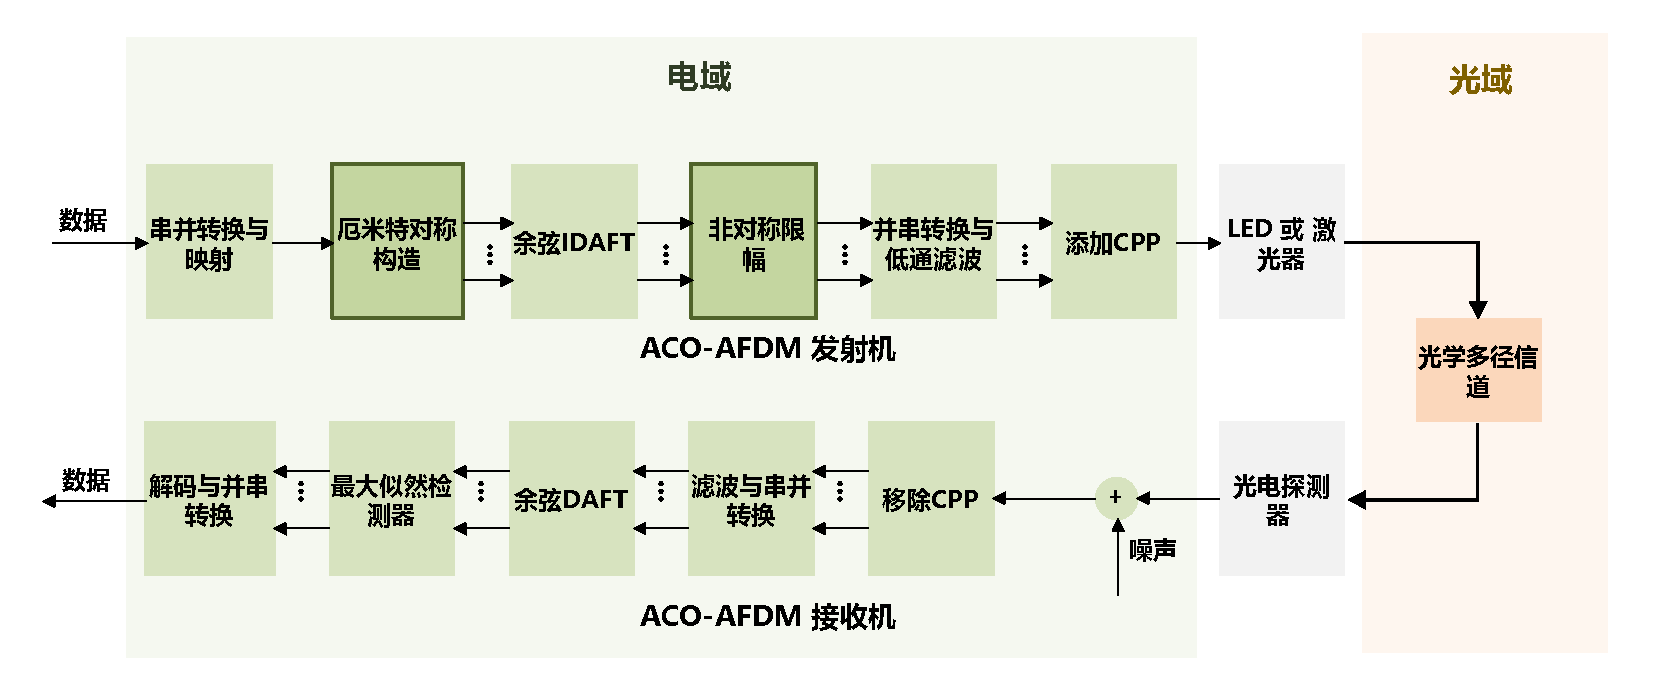
\includegraphics[width=1.0\linewidth]{figures/fig1_aco_afdm_system.pdf}
    \caption{ACO-AFDM 系统完整框图}
    \label{fig:aco_afdm_flow}
\end{figure}

从系统功能划分看，发射端主要完成比特映射、奇数位置加载、厄米特对称构造、AFDM 调制与非对称限幅；信道部分刻画低动态水下环境中的多径传播效应；接收端则完成前缀去除、变换域恢复、等效信道补偿与数据检测。通过这种设计，系统在满足光学发射物理约束的同时，可利用 AFDM 的结构优势增强对散射主导多径失真的适应能力。

\subsection{发射端信号生成与调制}
\label{subsec:aco_afdm_tx}

在发射端，输入比特首先映射为复数星座符号。为保证时域信号为实数，频域符号序列需满足厄米特对称条件。为避免限幅噪声落入承载数据信息的位置，ACO-AFDM 采用奇数子载波映射方式，即仅在奇数位置加载数据符号，偶数位置置零\cite{armstrongOFDMOpticalCommunications2009}。映射后的符号向量 $\mathbf{X}$ 表示为
\begin{equation}
    \mathbf{X} = [0, X_1, 0, X_3, \dots, X_{N/2-1}, 0, X_{N/2-1}^*, \dots, 0, X_3^*, 0, X_1^*]^T
\end{equation}

上述构造具有两个层面的作用。首先，厄米特对称保证经逆变换后得到的离散时域信号为实值，这是 IM/DD 系统可直接驱动光源的前提之一。其次，仅在奇数位置加载有效数据有助于在后续非对称限幅后将限幅噪声限制在偶数位置，从而避免其直接污染承载有效信息的变换域资源。因此，奇数子载波映射不仅是满足非负约束的技巧，也是一种围绕接收端可恢复性进行的结构化设计。

为将其映射到时域并保持实值特性，本文采用改进的余弦逆离散仿射傅里叶变换，其离散时域信号可表示为
\begin{equation}
    s[n] = \frac{1}{\sqrt{N}} \sum_{k=0}^{N-1} X[k] e^{j \frac{2\pi nk}{N}} \cos(2\pi c_1 n^2), \quad n=0,\dots,N-1
\end{equation}
其中，$c_1$ 为 DAFT 参数。本文令传统 AFDM 的第二参数 $c_2=0$，以保持半波反对称结构，即 $s[n] = -s[n+N/2]$。其矩阵形式可写为
\begin{equation}
    \mathbf{s} = \mathbf{C}\mathbf{F}^H \mathbf{X}
\end{equation}
其中，$\mathbf{C}$ 为由 $\cos(2\pi c_1 n^2)$ 构成的对角矩阵。

采用余弦型 DAFT 核的主要考虑在于，它能够在引入 AFDM 啁啾结构的同时保持时域实值信号特征，并与 ACO 机制所要求的半波反对称性质兼容。换言之，本文并不是简单将传统 AFDM 生硬套用于光学发射链路，而是围绕 IM/DD 约束对其变换核形式进行了有针对性的适配。参数 $c_1$ 的引入使信号在变换域中具备更适合多径分离的结构，而 $c_2=0$ 的设定则有助于维持 ACO 结构的可实现性和稳定性。

随后，对双极性时域信号进行非对称限幅，得到满足非负约束的发射信号
\begin{equation}
    s_{\mathrm{tx}}[n] = \max\{s[n], 0\}
\end{equation}
由于信号满足半波反对称性，限幅噪声仅分布于偶数子载波，不影响奇数子载波上的有效数据。最后，在每个信号块前添加长度为 $L_{\mathrm{cpp}}$ 的啁啾周期前缀，形成最终发射信号。

引入啁啾周期前缀的目的与传统循环前缀类似，都是为了抑制有限多径扩展导致的块间干扰，并为接收端的块处理恢复提供结构保证。不同之处在于，AFDM 调制后的信号具有啁啾相位特征，因此前缀设计需要与该结构保持一致。通过在块前添加适当长度的啁啾周期前缀，系统可在低动态多径条件下保持较稳定的块处理框架，从而为后续 DAFT 域恢复和信道均衡奠定基础。

\subsection{多径信道传播与接收端处理}
\label{subsec:aco_afdm_rx}

本文将低动态水下传播环境建模为具有 $P$ 条离散路径的时延抽头信道\cite{kaushalUnderwaterOpticalWireless2016a}。离散时间冲激响应可表示为
\begin{equation}
    h[n] = \sum_{i=1}^{P} h_i \delta[n-l_i]
\end{equation}
其中，$h_i$ 与 $l_i$ 分别表示第 $i$ 条路径的复增益和离散时延。接收端去除啁啾周期前缀后，接收信号向量为
\begin{equation}
    \mathbf{r} = \sum_{i=1}^{P} h_i \boldsymbol{\Pi}^{l_i}\mathbf{s}_{\mathrm{tx}} + \mathbf{w}
\end{equation}
其中，$\boldsymbol{\Pi}^{l_i}$ 为 $l_i$ 阶循环移位矩阵，$\mathbf{w}$ 为加性高斯白噪声。

上述模型反映了本文所关注的低动态场景的主要物理特征：路径之间的差异主要体现为传播时延和幅相响应差异，而由相对运动导致的时间快速变化可以近似忽略。因此，该信道更接近“准静态多径”而非“强时变双选择性”结构。尽管如此，当路径时延跨越多个采样间隔、且不同路径功率分布不均匀时，接收端仍会观察到显著的频率选择性衰落。这也是本章重点关注多径适应能力而非多普勒鲁棒性的原因。

接收端随后采用对应的余弦 DAFT 变换将信号恢复至仿射频域：
\begin{equation}
    Y[k] = \frac{1}{\sqrt{N}} \sum_{n=0}^{N-1} r[n] e^{-j \frac{2\pi nk}{N}} \cdot \frac{1}{\cos(2\pi c_1 n^2)}
\end{equation}
其矩阵形式为
\begin{equation}
    \mathbf{Y} = \mathbf{F}\mathbf{C}^{-1}\mathbf{r}
\end{equation}
由上述接收模型可知，系统在仿射频域中的恢复结果同时受多径卷积与限幅结构影响。在获得等效信道矩阵估计值 $\hat{\mathbf{H}}$ 后，可采用最大似然检测恢复原始数据符号。

从检测角度看，所提方案与传统 ACO-OFDM 的区别不仅体现在变换核不同，还体现在等效信道表示的结构差异。由于 AFDM 啁啾映射改变了路径时延在变换域中的投影形式，接收信号中的多径耦合不再表现为简单的傅里叶域子载波响应变化，而是体现为更具结构性的等效分布。这种结构差异为接收端进行更有针对性的均衡与检测提供了可能，也正是 ACO-AFDM 获得多径性能增益的关键所在。

\subsection{系统模型特点分析}
\label{subsec:aco_afdm_features}

综合发射端、信道与接收端结构，可以看出所提 ACO-AFDM 系统具有以下几个特点。

其一，系统在 IM/DD 架构下保持了实值非负发射的可实现性。通过厄米特对称、奇数位置加载和非对称限幅，发射端能够在不引入直流偏置的情况下满足光源驱动要求，并避免有效数据直接落入限幅噪声主分量所在位置。

其二，系统在保持 ACO 结构优势的同时，引入了 AFDM 的啁啾调制特性，使信号在面对低动态多径信道时能够在变换域中获得更适合描述路径结构的表示形式。相比传统 ACO-OFDM，这种结构更有利于减轻频率选择性衰落对局部资源位置的集中影响。

其三，系统的参数设计与接收端恢复过程存在显式耦合关系。特别是啁啾参数 $c_1$ 的选择不仅影响发射端变换实现，还直接决定接收端反变换的稳定性以及多径分量在 DAFT 域中的分布状态。因此，后续参数设计不能仅从数学可逆性出发，还需要同时考虑多径分离与实际检测性能。

基于上述特点，ACO-AFDM 并非简单地将 ACO 与 AFDM 两种机制进行形式叠加，而是在低动态多径 UWOC 场景下，围绕 IM/DD 发射约束、多径传播特性与接收恢复需求所形成的一种联合设计方案。

\section{ACO-AFDM 啁啾参数设计与全分集增益}
\label{sec:aco_afdm_params}

AFDM 的性能在较大程度上取决于啁啾参数设计。对于本文所提 ACO-AFDM 系统，参数 $c_1$ 的选择需同时满足逆变换稳定性与多径分离能力要求。由于本文采用余弦型 DAFT 核，参数设计不仅关系到信号在变换域中的分布形态，还直接影响接收端恢复过程中是否会出现数值不稳定或噪声增强现象。因此，有必要从奇异点规避与多径分离两个方面对其进行分析。

\subsection{奇异点规避准则}
\label{subsec:singularity_avoidance}

由接收端恢复公式可知，分母项中包含 $\cos(2\pi c_1 n^2)$。为避免逆变换过程中出现零点或过小值导致的噪声放大，需要满足
\begin{equation}
    2\pi c_1 n^2 \neq \frac{\pi}{2} + m\pi, \quad m \in \mathbb{Z}
\end{equation}
等价地，有
\begin{equation}
    c_1 \neq \frac{1/4 + m/2}{n^2}, \quad m \in \mathbb{Z}
    \label{eq:singularity_condition}
\end{equation}
因此，在参数选择时应剔除上述无效取值点。

这一约束的物理意义在于，余弦型 DAFT 核中包含的幅度调制项若在某些离散采样点附近接近零值，将使接收端在执行逆变换时对应位置的噪声被显著放大，进而导致整体检测性能恶化。换言之，即使某些参数在理论上并不破坏映射关系，只要其使 $\cos(2\pi c_1 n^2)$ 过小，也会降低系统实现稳定性。因此，奇异点规避不仅是数学层面的可逆性要求，也是工程实现中的数值稳健性要求。

在实际设计中，还应注意“避开严格零点”与“避开过小值区域”之间存在差异。前者保证逆变换在理论上可定义，后者则更贴近有限精度运算和实际噪声环境下的性能需求。因而，在候选参数搜索时，通常需要为 $\cos(2\pi c_1 n^2)$ 设定适当的安全裕量，而不是仅仅排除解析意义下的奇异取值点。

\subsection{多径分离与分集准则}
\label{subsec:multipath_separation}

为实现多径分量在 DAFT 域中的有效分离，需要考察路径时延引起的位置偏移。对于第 $i$ 条路径，其在 DAFT 域中的对称偏移位置可表示为
\begin{equation}
    \mathrm{loc}_i = (2N c_1 l_i)_N, \quad \mathrm{loc}_i^{\prime} = (-2N c_1 l_i)_N
\end{equation}
其中，$(\cdot)_N$ 表示模 $N$ 运算。

为避免不同路径在 DAFT 域中发生位置重叠，对于任意 $i \neq j$，需满足
\begin{equation}
    \{ \mathrm{loc}_i, \mathrm{loc}_i^{\prime} \} \cap \{ \mathrm{loc}_j, \mathrm{loc}_j^{\prime} \} = \emptyset
\end{equation}
若最大时延扩展为 $l_{\max}$，则为保证全部偏移范围不超过 DAFT 域长度 $N$，应满足
\begin{equation}
    4N c_1 l_{\max} \leq N
\end{equation}
由此得到参数边界
\begin{equation}
    0 < c_1 \leq \frac{1}{4 l_{\max}}
    \label{eq:c1_boundary}
\end{equation}
当 $c_1$ 同时满足式(\ref{eq:singularity_condition}) 与式(\ref{eq:c1_boundary}) 时，系统可在保证逆变换稳定性的同时提高对多径分量的分离能力。

上述准则说明，啁啾参数并不是越大越好或越小越好，而是需要在“增强路径可分辨性”和“控制变换域重叠风险”之间取得平衡。当 $c_1$ 过小时，不同路径在 DAFT 域中的偏移量较小，可能不足以体现 AFDM 对多径结构的区分优势；当 $c_1$ 过大时，路径对应响应又可能由于周期性折返而发生重叠，从而削弱系统的结构化表示能力。因此，合理参数区间本质上来自多径分离需求与有限离散维度约束的共同作用。

从分集利用角度看，若不同路径在 DAFT 域中能够保持较好的可区分性，则接收端在检测时更容易利用多径传播所提供的结构差异，而不是将其完全视作干扰源。这意味着，多径分量不再只是造成性能下降的失真项，也可能在合理波形设计下转化为可被利用的分集资源。本文所讨论的参数设计准则，正是为了使 ACO-AFDM 在低动态多径场景中尽可能保留这种结构性收益。

\subsection{参数设计的工程含义与取值权衡}
\label{subsec:param_tradeoff}

除上述理论约束外，参数 $c_1$ 的实际选取还应结合系统维度、最大时延扩展估计精度以及接收端复杂度进行综合考虑。对于较小的系统维度 $N$，可供选择的离散参数空间相对有限，若同时要求严格规避奇异点和路径重叠，则可行参数集合可能明显收缩；而当 $N$ 较大时，系统具有更细粒度的参数调节空间，但实现复杂度和前缀开销也可能随之上升。

此外，参数设计通常依赖对最大时延扩展 $l_{\max}$ 的先验估计。若该估计偏小，则依据式(\ref{eq:c1_boundary}) 选择的参数可能在真实信道下导致路径响应重叠；若估计偏大，则参数设置又可能过于保守，使 AFDM 的结构优势不能充分发挥。因此，在实际系统中，参数设计往往需要在鲁棒性与性能增益之间留出一定裕量。

从实现角度看，本文采用的参数设计并不追求全局最优，而是强调“可实现、可解释、与场景相适配”的选择原则。对于硕士论文层面的系统设计而言，这种基于物理约束和结构分析得到的参数准则具有较好的理论完整性与工程合理性，也为后续仿真设置提供了依据。

\section{仿真结果与分析}
\label{sec:aco_afdm_sim}

为验证所提 ACO-AFDM 方案在低动态多径水下场景中的性能，本节采用蒙特卡罗方法开展仿真，并与 ACO-OFDM、U-OFDM 以及 DCO-OFDM 进行对比\cite{dissanayakeComparisonACOOFDMDCOOFDM2013, fernandoFlipOFDMUnipolarCommunication2011}。

在仿真设置中，各方案均采用 $N=256$ 的子载波配置与 16-QAM 调制方式，并在接收端采用最大似然检测。针对所提 ACO-AFDM 方案，依据参数设计准则取 $c_1 = 1/(8l_{\max})$。水下多径信道建模为具有指数衰减功率延迟分布的离散瑞利信道。

上述设置旨在保证不同方案之间的可比性。统一的调制阶数和资源维度使性能差异主要来源于波形结构及其对多径传播的适应能力，而不是由参数不一致带来的额外偏差。同时，采用指数衰减型功率延迟分布能够较好反映低动态散射环境中“主路径较强、延迟路径逐步衰减”的典型传播特征，从而使仿真结论更贴近本文讨论的代表性应用条件。

\begin{figure}[htbp]
    \centering
    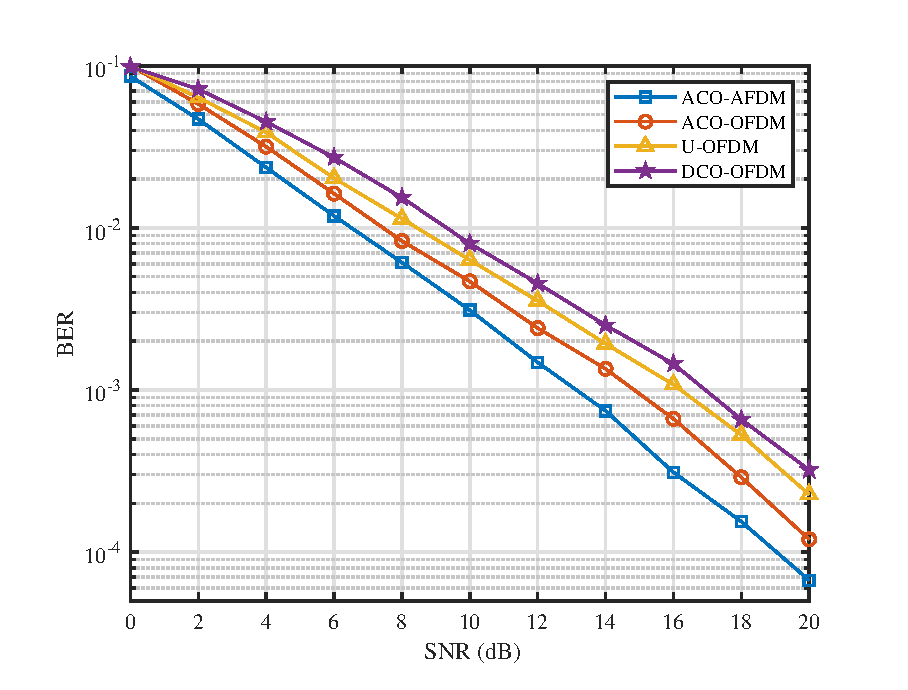
\includegraphics[width=0.85\linewidth]{figures/fig2_aco_afdm_ber_2path.eps}
    \caption{不同多载波方案在两径信道下的误码率性能对比}
    \label{fig:ber_comparison_2path}
\end{figure}

图~\ref{fig:ber_comparison_2path} 给出了最大时延扩展 $l_{\max}=10$ 采样周期时，各方案的 BER 与 SNR 关系曲线。由图可见，所提 ACO-AFDM 方案在整个观测 SNR 区间内均优于对比方案。在 $\mathrm{BER}=10^{-3}$ 附近，相较于 ACO-OFDM 可获得约 2 dB 的性能增益，说明所提方案在低动态多径条件下具有较好的误码率性能。

这一结果表明，在低动态 UWOC 中，系统性能的关键不完全取决于发射信号是否满足非负约束，还与波形对多径传播的适应能力密切相关。ACO-OFDM、U-OFDM 与 DCO-OFDM 虽然都能够实现单极性光信号传输，但它们在本质上仍主要依赖傅里叶域正交结构，因此当时延扩展引起明显频率选择性衰落时，部分资源位置会更易遭受性能退化。相比之下，ACO-AFDM 通过 DAFT 域中的结构化表示，使接收端能够更有效地应对多径导致的能量分散与局部深衰落问题，因此在相同信噪比条件下表现出更低的误码率。

需要注意的是，在较低 SNR 区间内，各方案之间的差距相对有限。这是因为噪声在此时仍是影响误码性能的主要因素，波形结构优势尚未充分显现；随着 SNR 提高，噪声影响逐渐减弱，信道结构与波形匹配关系开始主导系统性能，此时 ACO-AFDM 相对于传统光 OFDM 体制的优势更加明显。这一趋势与本文前述理论分析相一致。

\begin{figure}[htbp]
    \centering
    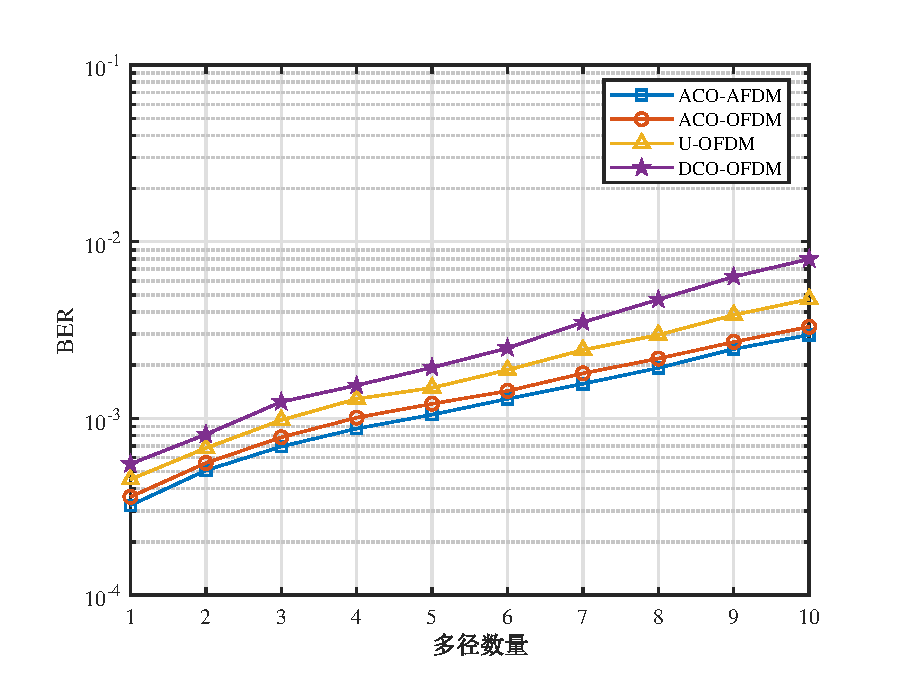
\includegraphics[width=0.85\linewidth]{figures/fig3_aco_afdm_ber_multipath.eps}
    \caption{多径路径数量对系统误码率性能的影响}
    \label{fig:multipath_robustness}
\end{figure}

图~\ref{fig:multipath_robustness} 给出了固定 $\mathrm{SNR}=16\,\mathrm{dB}$ 条件下，系统误码率随多径路径数变化的结果。由图可见，随着路径数量增加，传统 ACO-OFDM 与 U-OFDM 方案的误码率明显恶化，而 ACO-AFDM 的性能退化相对较缓。这表明所提方案对低动态水下多径传播具有更好的适应能力。

从机理上看，路径数增加意味着系统接收到更多延迟分量，频率选择性衰落程度加深，且不同路径之间的叠加关系更加复杂。对于传统光 OFDM 方案而言，这通常意味着子载波间信道增益差异增大、部分频率位置出现更严重的深衰落，从而使整体检测性能明显下降。而对于 ACO-AFDM，由于啁啾参数设计使多径响应在 DAFT 域中更具结构性，新增路径带来的影响并不完全等价于“更多随机干扰”，而是在一定程度上仍可通过结构化表示进行处理，因此其误码率退化速度较慢。

上述结果还说明，所提方案的性能优势并非仅体现在单一固定信道条件下，而是在多径复杂度变化时仍具有一定稳健性。这一点对于实际 UWOC 系统尤为重要，因为不同海域环境、不同水体浑浊程度以及不同收发几何条件下的路径数量和功率分布往往并不稳定。若一种传输方案仅在理想双径条件下有效，其工程适用性将受到明显限制；而 ACO-AFDM 在多路径数变化下仍保持相对稳定的性能表现，说明其更适合作为低动态多径场景下的候选物理层方案。

\subsection{结果讨论}
\label{subsec:aco_afdm_discussion}

综合上述仿真结果可以看出，所提 ACO-AFDM 方案在低动态多径 UWOC 场景下相较传统光 OFDM 方案具有更好的 BER 性能和多径鲁棒性。其优势主要来自以下几个方面：首先，ACO 结构保证了发射信号能够满足 IM/DD 架构的非负实值约束，并维持较好的光功率利用效率；其次，AFDM 啁啾映射增强了系统对多径传播结构的适应能力，使信号在变换域中的表示更有利于路径分离与检测；再次，合理的啁啾参数设计使系统在逆变换稳定性与多径分离能力之间取得了较好平衡。

进一步来看，所提方案的价值并不仅在于相较 ACO-OFDM 获得若干分贝的性能增益，更在于其揭示了一条适用于低动态 UWOC 的设计思路：即在 IM/DD 非负约束不可回避的前提下，可以通过对波形结构进行重新设计，而不是仅依赖传统 OFDM 框架下的局部修正，来提升系统对散射主导多径环境的适应能力。这种思路与本文全文所强调的“围绕场景特征对 AFDM 进行适配”的主线保持一致。

从本章研究过程可以进一步归纳出，所提方案在系统层面完成了三个相互关联的工作：一是在模型构建上，将奇数子载波映射、厄米特对称、余弦型 AFDM 调制与非对称限幅机制统一到 IM/DD 发射框架中，建立了适用于低动态多径水下光链路的收发模型；二是在参数设计上，围绕余弦型 DAFT 核分析了奇异点规避与多径分离条件，明确了啁啾参数的选取依据；三是在性能层面，通过 BER 与多径鲁棒性仿真验证了该方案在满足非负实信号约束的同时，能够较好提升系统对低动态多径传播的适应能力。由此可见，ACO-AFDM 并非对既有光 OFDM 结构的简单替换，而是面向低动态 UWOC 场景所形成的一种具有明确物理约束、参数依据与性能支撑的联合设计方案。

当然，所提方案也存在一定局限性。首先，本文仿真主要基于离散多径模型与理想同步假设展开，尚未进一步考虑更复杂的发射器非线性、接收器响应带宽限制及更强随机湍流扰动等因素；其次，参数设计在一定程度上依赖对最大时延扩展的先验估计，当信道统计特性明显偏离设计条件时，系统性能可能受到影响；再次，本文重点讨论误码率性能，对硬件实现复杂度、前缀开销和峰均功率比等工程指标尚未展开更深入分析。这些问题都可作为后续研究的拓展方向。

\chapter{面向高动态水下场景的相干 AFDM-IM 传输方案}
\label{chap:coherent_afdm_im}

面向高动态水下通信需求，UWOC 链路正由低动态准静态应用逐步向高速机动、强时变场景扩展\cite{hoeherUnderwaterOpticalWireless2021, MianXiangUUVJiQunYingYongDeShuiXiaWuXianGuangTongXinGuanJianJiShu2025}。在此类条件下，平台相对运动引起的多普勒频移会破坏传统 OFDM 子载波正交关系，导致严重载波间干扰\cite{zhuDopplerResistantOrthogonalChirp2022, fernandesDigitallyMitigatingDoppler2023}；同时，相干接收架构中发射与本振激光器的有限线宽还将引入维纳相位噪声\cite{tangUnderwaterCoherentOptical2021, huPerformanceCoherentOptical2025}，使接收端面临多普勒扩展与相位漂移的联合失真。传统 IM-DD 多载波体制由于仅能利用光强维度，难以同时兼顾接收灵敏度、抗多普勒能力与高阶调制需求\cite{liuMultiDegreeofFreedomUnderwaterOptical2022}。

AFDM 基于 DAFT 构造正交啁啾基函数，使时延与多普勒扩展在等效表示域中呈现结构性耦合形式，在双选择性信道中具有显著的鲁棒性优势\cite{bemaniAFDMFullDiversity2021, taoAffineFrequencyDivision2025}。相干探测能够恢复信号的幅度与相位信息，在接收灵敏度与背景噪声抑制方面具有优势，更适合支撑复数域 AFDM 传输\cite{guiomarCoherentFreeSpaceOptical2022, huPerformanceCoherentOptical2025}。在此基础上引入索引调制机制，通过激活位置与星座符号联合承载信息，可在提高比特映射效率的同时引入块稀疏结构\cite{basarOrthogonalFrequencyDivision2013, taoAffineFrequencyDivision2025}。更重要的是，AFDM-IM 中天然存在的大量未激活位置在理想情况下应保持为零，这些静默位置不仅服务于索引信息传输，还能够在接收端转化为可用于残余频偏感知的隐式结构参考，使索引调制从单纯的频谱效率提升工具进一步演化为接收端结构自感知的波形设计资源。

基于上述分析，本文提出相干 AFDM-IM 传输方案，建立包含多径、多普勒频移与维纳相位噪声的系统模型，推导 DAFT 域等效输入输出关系；进一步利用 AFDM-IM 静默位置所蕴含的零结构先验，研究基于静默位置泄露能量最小化与稀疏度量驱动的盲/半盲残余 CFO 补偿与检测方法。该思路将 IM 从单纯增谱效工具提升为接收端结构自感知资源，在减少显式导频开销的同时提高系统对残余频偏失配的适应能力，并对维纳相位噪声实现鲁棒容忍。

\section{相干 AFDM-IM 系统模型构建}
\label{sec:coherent_afdm_im_model}

本节在第二章双选择性信道模型与 AFDM 基本原理基础上，建立相干 AFDM-IM 系统的发射端、信道与接收端模型。系统完整框图如图~\ref{fig:coherent_afdm_im_system} 所示。与第三章的 ACO-AFDM 方案不同，本章采用相干光架构直接传输复数域 AFDM-IM 基带信号。

\begin{figure}[htbp]
    \centering
    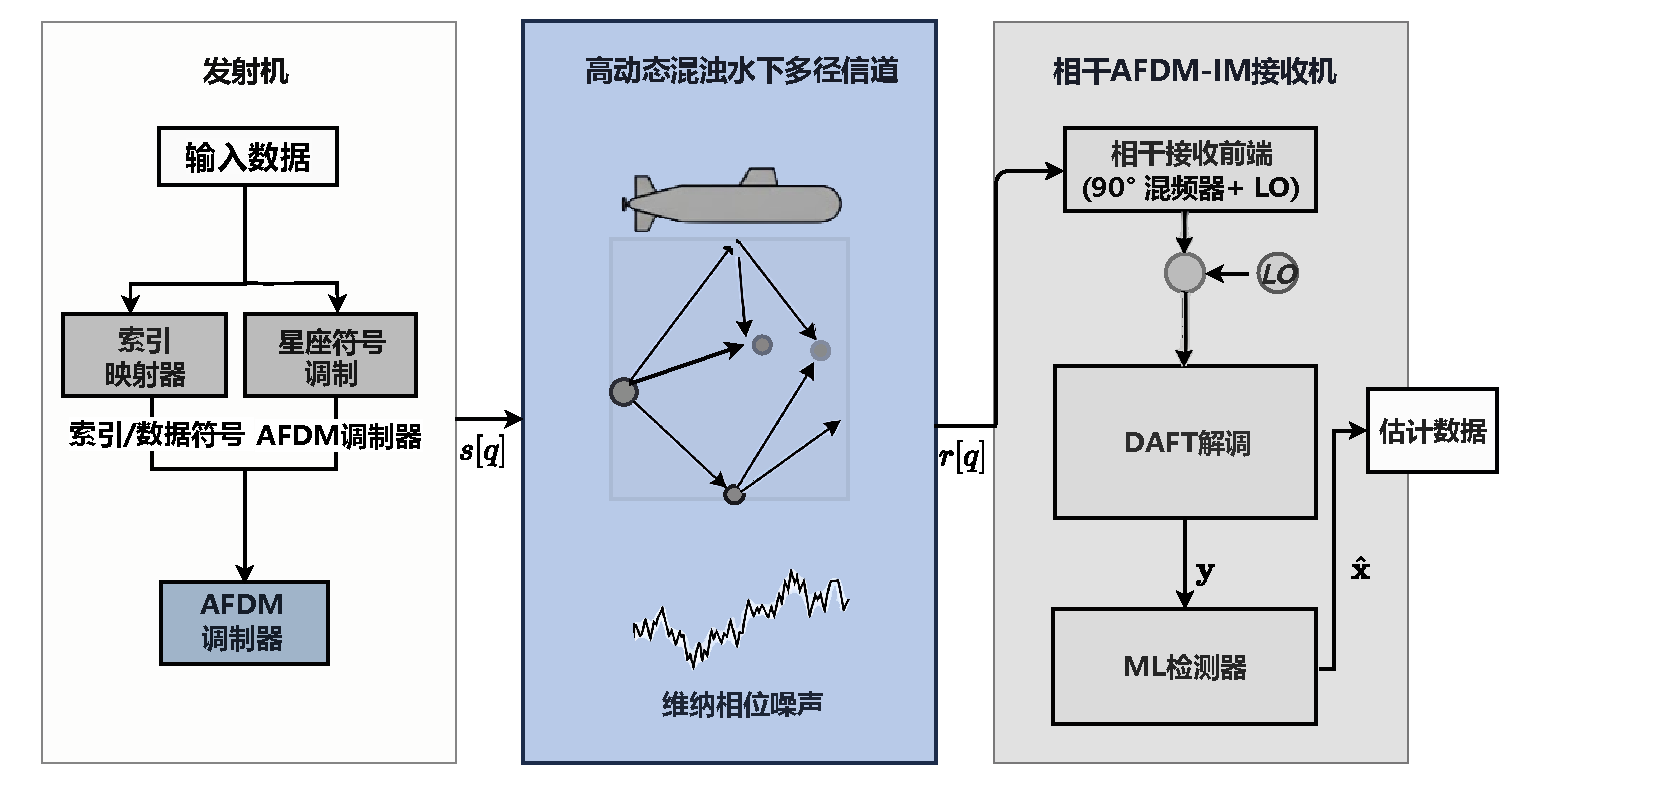
\includegraphics[width=0.85\linewidth]{figures/fig5_coherent_system.pdf}
    \caption{相干 AFDM-IM 系统完整框图}
    \label{fig:coherent_afdm_im_system}
\end{figure}

在系统整体设计上，本文将 AFDM 波形、相干接收和索引调制结构联合考虑。其基本思路是：在发射端利用 AFDM 的啁啾基构造提高系统对双选择性信道的适应能力，在符号层面通过索引调制机制引入块稀疏结构，以兼顾信息承载效率和检测复杂度；在接收端则借助相干探测恢复复数基带信号，并在 DAFT 域下建立统一的等效输入输出关系。通过这种联合设计，系统不仅能够适配高动态场景下的时延与多普勒耦合特征，还能为后续检测方法提供模型基础。

\subsection{发射端 AFDM-IM 信号构造}
\label{subsec:coherent_afdm_im_tx}

设系统总 DAFT 域维度为 $N$，将其划分为 $G$ 个等长子块，则每个子块长度为 $n=N/G$。对于第 $g$ 个子块，输入比特分为索引比特与星座比特两部分。若每个子块中有 $k$ 个激活位置，则索引比特数与星座比特数分别为
\begin{equation}
    b_{\mathrm{I}} = \left\lfloor \log_2 \binom{n}{k} \right\rfloor,
    \qquad
    b_{\mathrm{S}} = k \log_2 M
    \label{eq:im_bits_mapping}
\end{equation}
其中，$M$ 为复星座调制阶数。因此，每个子块承载的总比特数为 $b_g=b_{\mathrm{I}}+b_{\mathrm{S}}$。

上述分块设计的意义在于在频谱效率、结构稀疏性与检测复杂度之间取得平衡。若直接在整个长度为 $N$ 的向量上进行全局索引映射，虽然能够获得更大的激活模式集合，但接收端的候选搜索空间也会迅速膨胀；而将发送向量划分为多个等长子块后，可在保持较高比特承载能力的同时，将检测问题限制在局部维度上。参数 $n$、$k$ 与 $G$ 的选取因此具有明确物理意义：$n$ 决定单个子块的判决维度，$k$ 反映每个子块的激活稀疏程度，$G$ 则决定整帧中并行信息单元的数量。三者共同影响系统频谱效率、误码性能以及接收端复杂度。

记第 $g$ 个子块的 AFDM-IM 向量为 $\mathbf{x}_g \in \mathbb{C}^{n\times 1}$。其非零位置由索引集合 $\mathcal{I}_g$ 确定，其中
\begin{equation}
    \mathcal{I}_g=\{i_{g,1},i_{g,2},\ldots,i_{g,k}\}
\end{equation}
于是
\begin{equation}
    x_g[m] =
    \begin{cases}
        s_{g,u}, & m = i_{g,u},\; u=1,2,\ldots,k \\
        0, & m \notin \mathcal{I}_g
    \end{cases}
    \label{eq:subblock_im_vector}
\end{equation}
其中，$s_{g,u}\in\mathcal{S}$，$\mathcal{S}$ 表示 $M$ 阶复星座集合。将全部子块顺序拼接，可得到整帧 DAFT 域发送向量
\begin{equation}
    \mathbf{x} = [\mathbf{x}_1^T,\mathbf{x}_2^T,\ldots,\mathbf{x}_G^T]^T \in \mathbb{C}^{N\times 1}
    \label{eq:global_im_vector}
\end{equation}
其满足块稀疏约束 $\|\mathbf{x}_g\|_0=k$。

由上述结构可见，AFDM-IM 的信息承载由两部分共同组成：一部分由激活位置决定，对应索引比特；另一部分由激活位置上的复星座符号决定，对应星座比特。这种联合映射方式使系统在单位资源下可传输的信息量超过单纯依赖星座点的常规调制方式。同时，由于非激活位置保持为零，发送向量天然具有块稀疏特征，这也为后续最大似然检测提供了结构基础。图~\ref{fig:sim_bit_mapping_structure} 从比特分流与子块激活结构两个角度，对 AFDM-IM 的发送向量构造过程进行了直观说明。

\begin{figure}[htbp]
    \centering
    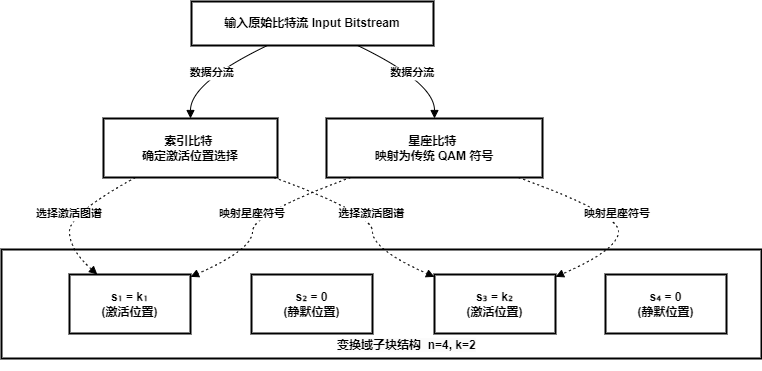
\includegraphics[width=0.82\linewidth]{figures/fig4_1_sim_bit_mapping_structure.png.png}
    \caption{AFDM-IM 子块比特映射与静默位置结构示意图}
    \label{fig:sim_bit_mapping_structure}
\end{figure}

\subsubsection{AFDM-IM 频谱效率分析}

为定量衡量所提 AFDM-IM 方案的信息承载能力，本节对其频谱效率进行分析，并与常规 AFDM（不采用索引调制）和传统 OFDM-IM 进行对比。

对于 AFDM-IM，系统每帧承载的总比特数为
\begin{equation}
    B_{\mathrm{AFDM\text{-}IM}} = G \cdot \left(\left\lfloor \log_2 \binom{n}{k} \right\rfloor + k\log_2 M\right)
    \label{eq:afdm_im_total_bits}
\end{equation}
而对于不采用索引调制的常规 AFDM，全部 $N$ 个 DAFT 域位置均加载星座符号，每帧承载比特数为
\begin{equation}
    B_{\mathrm{AFDM}} = N \log_2 M
    \label{eq:afdm_total_bits}
\end{equation}

以本章仿真参数为例（$N=256$，$G=32$，$n=8$，$k=2$，$M=4$），代入式(\ref{eq:afdm_im_total_bits}) 可得
\begin{equation}
    B_{\mathrm{AFDM\text{-}IM}} = 32 \times \left(\lfloor\log_2 28\rfloor + 2\times 2\right) = 32 \times (4+4) = 256 \text{ bit/帧}
\end{equation}
对应的归一化频谱效率为 $\eta_{\mathrm{AFDM\text{-}IM}} = 256/(256+L_{\mathrm{cp}}) \approx 0.96$ bit/s/Hz（取 $L_{\mathrm{cp}}=10$）。作为对比，常规 AFDM 的每帧比特数为 $B_{\mathrm{AFDM}} = 256 \times 2 = 512$ bit/帧，频谱效率约为 1.92 bit/s/Hz。

从上述数值可以看出，AFDM-IM 的频谱效率约为常规 AFDM 的 50\%。然而，这一对比并不构成 AFDM-IM 的劣势，原因在于：索引调制以降低绝对频谱效率为代价，换取了以下三方面收益。一是接收端检测可靠性的提升——由于每个子块仅有 $k$ 个激活位置，ML 检测的候选空间从 $M^n$ 压缩为 $\binom{n}{k}M^k$，搜索范围显著缩小，判决可靠性在有限信噪比下得以改善。二是发射信号平均功率的降低——在每个子块的 $n$ 个位置中仅 $k$ 个承载非零符号，在总能量约束下单个激活位置可分配到更高的瞬时功率，从而提高单符号信噪比。三是静默位置为接收端提供了可利用的结构先验——这正是本章后续基于静默位置泄露能量最小化方法的物理基础。

与传统 OFDM-IM 相比，AFDM-IM 在相同子块划分和激活参数下具有相同的索引比特数 $b_{\mathrm{I}}$ 和星座比特数 $b_{\mathrm{S}}$，因此两者的频谱效率完全相同。二者的性能差异完全来源于波形结构层面：AFDM 的啁啾映射使系统在高动态双选择性信道下保持更好的结构稳定性，而 OFDM 在同等多普勒条件下会因子载波正交性破坏导致严重的 ICI。进一步地，不同子块映射模式 $(n,k)$ 还会影响索引效率、平均激活能量和检测鲁棒性之间的权衡。图~\ref{fig:sim_subblock_modes} 给出了若干典型映射模式下的 BER 对比结果，可用于说明本章后续仿真中采用固定子块结构的设计依据。

\begin{figure}[htbp]
    \centering
    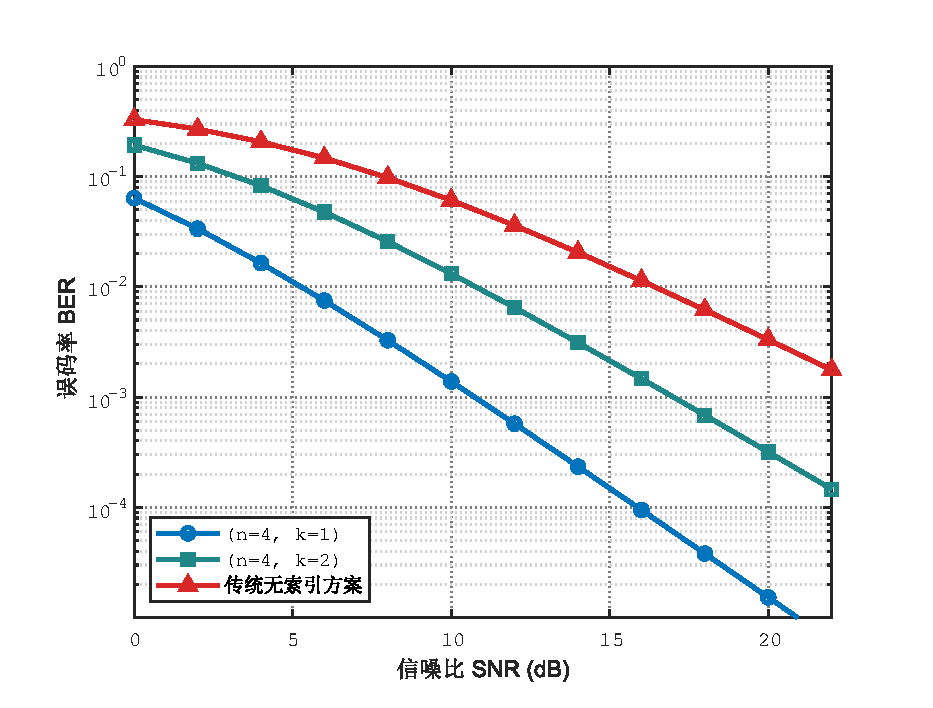
\includegraphics[width=0.85\linewidth]{figures/fig4_4_ber_sim_subblock_modes.eps}
    \caption{不同子块映射模式 $(n,k)$ 下相干 AFDM-IM 系统的 BER 性能对比}
    \label{fig:sim_subblock_modes}
\end{figure}

发送向量经离散逆仿射傅里叶变换映射至时域。记 AFDM 调制矩阵为
\begin{equation}
    \boldsymbol{\Psi} = \boldsymbol{\Lambda}_{c_1}^{H} \mathbf{F}^{H} \boldsymbol{\Lambda}_{c_2}^{H}
    \label{eq:afdm_mod_matrix}
\end{equation}
其中，$\mathbf{F}$ 为归一化 DFT 矩阵，$\boldsymbol{\Lambda}_{c_1}$ 与 $\boldsymbol{\Lambda}_{c_2}$ 分别为由啁啾参数 $c_1$ 和 $c_2$ 决定的对角相位矩阵。则离散时域基带信号为
\begin{equation}
    \mathbf{s} = \boldsymbol{\Psi}\mathbf{x}
    \label{eq:tx_signal_vector}
\end{equation}
为抑制多径引起的块间干扰，在每个 AFDM 符号前添加长度为 $L_{\mathrm{cp}}$ 的循环前缀。由于采用相干架构，发送端可直接加载复数包络信号，因此无需进行厄米特对称映射与非负限幅处理。

相较于 IM-DD 架构下对实值非负性的严格约束，相干架构允许发送端直接处理复数域波形，因此 AFDM 的复数调制优势能够得到更充分体现。另一方面，循环前缀的引入使系统在面对有限时延扩展时仍可维持较稳定的块处理结构，为后续在 DAFT 域中建立等效输入输出关系提供了前提。由此可见，AFDM-IM 发射端并不是对 AFDM 和索引调制的简单叠加，而是在高动态相干场景下对波形、映射和接收架构进行联合适配的结果。

\subsection{高动态水下相干光信道模型}
\label{subsec:coherent_afdm_im_channel}

考虑收发平台之间存在高速相对运动的高动态 UWOC 场景，信道可建模为具有 $P$ 条离散路径的线性时变系统。第 $p$ 条路径的复增益、离散时延和归一化多普勒频移分别记为 $h_p$、$l_p$ 和 $\alpha_p$。在去除循环前缀后，时域接收信号可表示为
\begin{equation}
    r[q] = e^{j\phi[q]} \sum_{p=1}^{P} h_p e^{j\frac{2\pi}{N}\alpha_p q} s[(q-l_p)_N] + w[q],
    \qquad q=0,1,\ldots,N-1
    \label{eq:time_domain_received_signal}
\end{equation}
其中，$w[q]$ 为零均值复高斯白噪声，$(\cdot)_N$ 表示模 $N$ 运算，$\phi[q]$ 表示由发射激光器与本振激光器有限线宽共同引起的离散相位噪声过程。由式(\ref{eq:time_domain_received_signal}) 可见，时域接收信号同时受到多径时延、多普勒旋转与相位噪声扰动的共同影响。

式(\ref{eq:time_domain_received_signal}) 中各参数具有明确的物理含义。$h_p$ 反映第 $p$ 条路径的复增益，既包含路径损耗信息，也包含由传播过程引起的相位变化；$l_p$ 描述离散时延，用于刻画不同路径的到达时间差；$\alpha_p$ 则表征归一化多普勒频移，用以描述相对运动导致的频率扩展效应。在高动态场景下，多个路径往往同时具有不同的时延与多普勒偏移，因此接收信号并非简单的时移叠加，而是带有时移--频移耦合特征的复合过程。

与低动态场景相比，高动态 UWOC 所面临的困难在于信道失真不再局限于静态多径扩展，而是表现为多径 + 多普勒 + 接收架构非理想的联合影响。若仅考虑多径效应，系统可通过前缀保护、变换域均衡等手段进行处理；但当多普勒扩展与器件相位不稳定性同时存在时，接收信号会出现更明显的能量扩散、星座旋转与等效信道失配，进而提高检测难度。因此，建立兼顾多径、多普勒和相位噪声的统一信道模型，对于后续算法设计具有基础性意义。

根据维纳相位噪声模型，离散相位过程满足
\begin{equation}
    \phi[q] = \phi[q-1] + \Delta[q],
    \qquad
    \Delta[q] \sim \mathcal{N}(0,\sigma_{\phi}^{2})
    \label{eq:phase_noise_process}
\end{equation}
其中，$\Delta[q]$ 为独立高斯增量，且有
\begin{equation}
    \sigma_{\phi}^{2} = 2\pi \Delta \nu T_s
    \label{eq:phase_noise_variance}
\end{equation}
其中，$\Delta\nu$ 为组合线宽，$T_s$ 为采样间隔。由式(\ref{eq:phase_noise_variance}) 可知，相位噪声方差与组合线宽和采样间隔成正比。

维纳相位噪声模型之所以适用于本文场景，是因为相干光系统中的发射激光器与本振激光器通常具有独立的相位漂移过程，其相位误差会在离散时间上呈现逐步累积的随机游走特征。组合线宽越大，相邻采样间的相位波动越强，因而更容易在接收端引起星座旋转和检测失配。对于高阶复数调制或长帧结构而言，这种累积效应会更加突出。特别是在多普勒扩展已经破坏部分结构稳定性的前提下，相位噪声的存在会进一步加剧等效信道不确定性，使接收端难以通过简单补偿获得理想性能。

将式(\ref{eq:time_domain_received_signal}) 写为矩阵形式，可得
\begin{equation}
    \mathbf{r} = \boldsymbol{\Phi} \sum_{p=1}^{P} h_p \boldsymbol{\Lambda}(\alpha_p) \boldsymbol{\Pi}^{l_p} \mathbf{s} + \mathbf{w}
    \label{eq:matrix_received_signal}
\end{equation}
其中，$\boldsymbol{\Phi}$ 为相位噪声对角矩阵，$\boldsymbol{\Lambda}(\alpha_p)$ 为多普勒旋转矩阵，$\boldsymbol{\Pi}^{l_p}$ 为循环移位矩阵。

上述矩阵形式表明，接收信号可以看作多个时移 + 多普勒旋转算子叠加后再经相位噪声扰动得到的结果。这种表示方式为后续将系统映射到 DAFT 域提供了便利，也说明高动态 UWOC 的检测问题实质上是一个在复合时变信道下的联合估计问题，而非简单的逐位置独立判决问题。

\subsection{接收端 DAFT 域等效输入输出关系}
\label{subsec:coherent_afdm_im_rx}

在接收端，去除循环前缀后的接收向量 $\mathbf{r}$ 经 AFDM 解调矩阵
\begin{equation}
    \boldsymbol{\Psi}^{H} = \boldsymbol{\Lambda}_{c_2} \mathbf{F} \boldsymbol{\Lambda}_{c_1}
    \label{eq:afdm_demod_matrix}
\end{equation}
处理后，得到 DAFT 域接收向量
\begin{equation}
    \mathbf{y} = \boldsymbol{\Psi}^{H} \mathbf{r}
    \label{eq:daft_received_signal}
\end{equation}
代入发送信号与信道模型后，可得
\begin{equation}
    \mathbf{y}
    =
    \boldsymbol{\Psi}^{H}
    \boldsymbol{\Phi}
    \sum_{p=1}^{P} h_p \boldsymbol{\Lambda}(\alpha_p) \boldsymbol{\Pi}^{l_p}
    \boldsymbol{\Psi}
    \mathbf{x}
    +
    \tilde{\mathbf{w}}
    \label{eq:equivalent_daft_io_1}
\end{equation}
其中，$\tilde{\mathbf{w}}=\boldsymbol{\Psi}^{H}\mathbf{w}$ 仍服从复高斯分布。进一步定义 DAFT 域等效信道矩阵为
\begin{equation}
    \mathbf{H}_{\mathrm{eq}}
    =
    \boldsymbol{\Psi}^{H}
    \boldsymbol{\Phi}
    \sum_{p=1}^{P} h_p \boldsymbol{\Lambda}(\alpha_p) \boldsymbol{\Pi}^{l_p}
    \boldsymbol{\Psi}
    \label{eq:equivalent_channel_matrix}
\end{equation}
则输入输出关系可统一表示为
\begin{equation}
    \mathbf{y} = \mathbf{H}_{\mathrm{eq}} \mathbf{x} + \tilde{\mathbf{w}}
    \label{eq:equivalent_daft_io_2}
\end{equation}
该式为后续检测算法推导奠定了基础，也表明检测问题可以统一表述为在等效 DAFT 域信道下对发送向量的估计问题。

\subsection{维纳相位噪声的结构化分解}
\label{subsec:phase_noise_decomposition}

式(\ref{eq:equivalent_channel_matrix}) 中的相位噪声对角矩阵 $\boldsymbol{\Phi} = \mathrm{diag}(e^{j\phi[0]}, e^{j\phi[1]}, \ldots, e^{j\phi[N-1]})$ 将维纳相位过程的逐点效应引入了等效信道表达。为后续算法设计提供理论支撑，有必要对符号周期内的维纳相位过程进行结构化分解，明确其各分量对检测性能的影响机理。

将维纳相位过程 $\phi[q]$（$q = 0, 1, \ldots, N-1$）在一个符号周期内进行正交分解：
\begin{equation}
    \phi[q] = \underbrace{\phi[0]}_{\text{常数相位}} + \underbrace{\frac{q}{N}\left(\phi[N-1]-\phi[0]\right)}_{\text{线性漂移}} + \underbrace{\epsilon[q]}_{\text{高阶随机残差}}
    \label{eq:phase_noise_decomposition}
\end{equation}
其中，三个分量具有不同的物理含义与对检测的影响方式。

常数相位分量 $\phi[0]$ 对整个符号块施加统一的相位旋转。由于最大似然检测中对发送向量的判决基于欧氏距离度量，而常数相位旋转等价于对接收信号向量进行全局旋转，不改变各候选向量与接收观测之间的距离排序，因此该分量对检测结果透明，无需显式补偿。

线性漂移分量 $\frac{q}{N}(\phi[N-1]-\phi[0])$ 在时域上表现为线性相位斜坡，其效果等价于一个小量的频率偏移。设线性漂移对应的等效归一化频偏为
\begin{equation}
    \Delta f_{\mathrm{drift}} = \frac{\phi[N-1]-\phi[0]}{2\pi}
    \label{eq:linear_drift_freq}
\end{equation}
由于 $\phi[N-1]-\phi[0] = \sum_{q=1}^{N-1}\Delta[q]$ 是 $N-1$ 个独立高斯增量的累加，其方差为 $(N-1)\sigma_\phi^2$。在典型参数条件下（$N=256$，$\Delta\nu T_s = 10^{-4}$），线性漂移分量的标准差约为 $\sqrt{(N-1) \cdot 2\pi \cdot 10^{-4}} \approx 0.40$ rad，对应的等效归一化频偏约为 $0.40/(2\pi) \approx 0.064$。该分量在形式上与残余 CFO 完全相同（均表现为时域线性相位），因此可被后续盲搜算法在搜索过程中自动吸收——算法所估计的"最优频偏补偿参数"实际上是真实 CFO 与线性漂移之和，二者无需分别处理。

高阶随机残差 $\epsilon[q]$ 是维纳相位过程去除常数和线性分量后的剩余部分，表现为零均值、时间相关的随机波动。其方差可通过布朗桥模型给出上界：
\begin{equation}
    \mathrm{Var}[\epsilon[q]] \leq \frac{q(N-1-q)}{N-1} \sigma_\phi^2
    \label{eq:residual_variance_bound}
\end{equation}
该上界在 $q = (N-1)/2$ 处取得最大值 $(N-1)\sigma_\phi^2/4$。在本文典型参数下，$\max_q \mathrm{Var}[\epsilon[q]] \approx 255 \times 2\pi \times 10^{-4}/4 \approx 0.040$ rad$^2$，对应的标准差约为 0.20 rad。

当残差相位较小时（$|\epsilon[q]| \ll 1$），可对相位噪声指数进行线性化近似：
\begin{equation}
    e^{j\epsilon[q]} \approx 1 + j\epsilon[q]
    \label{eq:phase_noise_linearization}
\end{equation}
该近似的有效条件为 $\mathrm{Var}[\epsilon[q]] \ll 1$ rad$^2$。在本文仿真条件下，最大残差方差为 0.040 rad$^2$，远小于 1，因此线性化近似成立。此时，高阶随机残差的效果等价于在接收信号上叠加一个功率受限的附加噪声项：
\begin{equation}
    e^{j\epsilon[q]} \cdot r_{\mathrm{comp}}[q] \approx r_{\mathrm{comp}}[q] + j\epsilon[q] \cdot r_{\mathrm{comp}}[q]
    \label{eq:residual_as_noise}
\end{equation}
其中 $r_{\mathrm{comp}}[q]$ 为经 CFO 补偿后的接收信号。第二项可视为信号依赖型附加噪声，其功率与信号功率和残差方差的乘积成正比。

上述分解的意义在于：维纳相位噪声中对检测性能影响最大的两个分量（常数相位和线性漂移）恰好分别被 ML 检测的距离度量不变性和盲搜算法的频偏吸收能力自动处理，而剩余的高阶随机残差在线性化近似下等效为功率受限的附加噪声。这一分析为后续将维纳相位噪声作为等效背景干扰纳入残余噪声项处理提供了严格的理论依据，也解释了为何所提算法能够在不显式估计完整维纳相位过程的情况下仍对相位噪声保持鲁棒容忍。

\subsection{DAFT 域等效信道矩阵的结构特性}
\label{subsec:daft_channel_structure}

为深入理解 AFDM 在高动态场景中的性能优势来源，本节对式(\ref{eq:equivalent_channel_matrix}) 所定义的 DAFT 域等效信道矩阵 $\mathbf{H}_{\mathrm{eq}}$ 的结构特性进行分析。

在不考虑相位噪声的理想条件下（即 $\boldsymbol{\Phi} = \mathbf{I}$），等效信道矩阵退化为
\begin{equation}
    \mathbf{H}_{\mathrm{eq}}^{(\mathrm{ideal})} = \boldsymbol{\Psi}^{H} \sum_{p=1}^{P} h_p \boldsymbol{\Lambda}(\alpha_p) \boldsymbol{\Pi}^{l_p} \boldsymbol{\Psi}
    \label{eq:ideal_equiv_channel}
\end{equation}

对于单条路径（$P=1$，$h_1=1$，$l_1=l$，$\alpha_1=\alpha$），利用 DAFT 调制矩阵的解析形式，可将等效信道矩阵的第 $(m,k)$ 元素表示为
\begin{equation}
    [\mathbf{H}_{\mathrm{eq}}^{(\mathrm{ideal})}]_{m,k} = h_1 \cdot \delta\!\left[(m - k - 2Nc_1 l - 2Nc_2\alpha)_N\right] \cdot e^{j\varphi_{m,k}}
    \label{eq:single_path_channel_element}
\end{equation}
其中 $\varphi_{m,k}$ 为与啁啾参数和路径参数相关的相位项，$\delta[\cdot]$ 为克罗内克 delta 函数。式(\ref{eq:single_path_channel_element}) 表明，单条路径在 DAFT 域中对应等效信道矩阵的一条对角线（偏移量为 $(2Nc_1 l + 2Nc_2\alpha)_N$）。

当存在多条路径时，等效信道矩阵为各路径贡献的叠加：
\begin{equation}
    \mathbf{H}_{\mathrm{eq}}^{(\mathrm{ideal})} = \sum_{p=1}^{P} h_p \cdot \mathbf{D}_p
    \label{eq:multipath_channel_superposition}
\end{equation}
其中 $\mathbf{D}_p$ 为第 $p$ 条路径对应的移位对角矩阵，其非零元素位于第 $(2Nc_1 l_p + 2Nc_2\alpha_p)_N$ 条对角线上。该结构具有以下重要性质。

当啁啾参数 $c_1$ 和 $c_2$ 设计合理时，不同路径对应的对角线偏移量相互区分，使等效信道矩阵呈现稀疏的多对角线结构。在这种条件下，DAFT 域中每个接收位置仅与有限个发送位置耦合，检测算法可利用这种稀疏性降低计算复杂度。当路径的时延-多普勒参数对满足分离条件
\begin{equation}
    (2Nc_1 l_p + 2Nc_2\alpha_p)_N \neq (2Nc_1 l_q + 2Nc_2\alpha_q)_N, \quad \forall p \neq q
    \label{eq:path_separation_condition_ch4}
\end{equation}
时，各路径在 DAFT 域中占据不同的对角线位置，接收端可通过结构化检测联合利用所有路径能量，获得满分集增益。

与 OFDM 的等效信道矩阵进行对比可进一步揭示 AFDM 的优势。对于 OFDM 系统，在无多普勒条件下，等效信道为对角矩阵，各子载波独立经历频率选择性衰落；当存在多普勒时，等效信道变为满矩阵（非稀疏），每个接收位置与所有发送位置耦合，产生全局性的 ICI。AFDM 则通过啁啾参数的引入，将时延-多普勒耦合映射为 DAFT 域中的确定性位置偏移，使等效信道在双选择性条件下仍保持稀疏结构，这正是其抗多普勒能力优于 OFDM 的根本原因。

\section{基于静默位置泄露能量最小化的残余 CFO 补偿与检测方法}
\label{sec:silent_leakage_phase_comp}

在上一节的系统模型中，时域接收信号同时受到多径时延、多普勒频移以及维纳相位噪声的联合影响。在高动态 UWOC 场景下，上述因素中对 DAFT 域子载波正交性破坏最为严重的是多普勒效应所引发的载波频率偏移（Carrier Frequency Offset, CFO）。载波频偏在时域表现为线性相位斜坡，经 DAFT 变换后会导致能量从激活位置大规模扩散至相邻位置，从而使原本应为零的静默位置上出现显著的残余能量——这正是静默位置泄露的核心物理来源。相比之下，维纳相位噪声虽然也会引起逐点时变的相位扰动，但其随机游走特性使其在单符号尺度上的主要效应表现为叠加在残余频偏之上的随机结构扰动，而非可由单一标量直接表征并完全补偿的确定性泄露来源。

基于上述物理认识，本节进一步利用 AFDM-IM 发送向量的块稀疏结构，构造一种基于静默位置泄露能量最小化的盲/半盲残余 CFO 补偿与检测方法。该方法不再将索引调制仅视为频谱效率增强手段，而是进一步把未激活位置所蕴含的零结构先验转化为接收端可利用的隐式参考信息，从而在减少或避免显式导频开销的前提下完成主导残余频偏分量的感知、补偿与后续检测。

本节将待估参数建模为归一化残余频率偏移 $\theta$，其物理意义对应于多普勒效应在接收端引起的等效载波频偏。由于维纳相位噪声是逐点时变的随机过程，无法被单一标量参数完全描述或消除，本文的算法框架将其视为等效背景干扰，与热噪声一并纳入残余噪声项处理。这一建模选择的合理性将通过后续仿真得到验证：算法能够精准补偿主导频偏分量，使系统 BER 显著优于传统导频方案；而由于残余维纳相位噪声的存在，系统相较于理想下界保留极小的性能折损，体现了工程上的合理鲁棒性。

\subsection{基本思想与问题建模}
\label{subsec:silent_leakage_principle}

对于第 $g$ 个子块，AFDM-IM 发送向量 $\mathbf{x}_g\in\mathbb{C}^{n\times 1}$ 满足稀疏激活约束 $\|\mathbf{x}_g\|_0=k<n$。若记其激活位置集合为 $\mathcal{I}_g$，则静默位置集合可写为 $\mathcal{Z}_g=\{1,2,\ldots,n\}\setminus\mathcal{I}_g$。理想情况下，对于任意 $m\in\mathcal{Z}_g$，均有
\begin{equation}
    x_g[m]=0.
\end{equation}
在无频偏且无相位噪声时，DAFT 域接收信号的能量将严格集中在激活位置上，静默位置保持为零。然而，当存在多普勒效应引起的载波频偏时，时域信号相当于被乘以线性相位斜坡 $e^{j2\pi\theta q/N}$（其中 $\theta$ 为归一化频偏参数），该线性相位在经过 DAFT 变换后会破坏子载波间的正交性，导致能量从激活位置向相邻位置大规模扩散，从而在静默位置上产生显著的残余分量。这种由频偏引起的载波间干扰（ICI）和能量泄露，正是静默位置泄露能量最小化准则所针对的核心失真。

为明确区分不同失真机制对能量泄露的贡献，可对接收端观测到的静默位置残余能量做如下定性分析。一方面，若仅存在恒定相位偏移 $e^{j\phi_0}$（即常数相位旋转），由于酉变换的保模性质，DAFT 域各位置的能量分布不会改变，静默位置仍为零——因此，纯常数相位不会引起能量泄露，也无法通过静默位置能量准则加以估计。另一方面，线性相位斜坡（即载波频偏）会在变换域引起系统性的子载波间能量扩散，其效应随频偏增大而显著增强，是能量泄露的主导来源。至于维纳相位噪声，由于其为逐采样点独立累积的随机游走过程，无法被任何单一标量参数所完整描述，其效应在本文算法框架中被归入等效残余干扰处理。

基于上述分析，本文将待估参数 $\theta$ 明确定义为归一化残余载波频偏。在高动态 UWOC 场景中，该参数主要源自收发平台相对运动所导致的多普勒频移。定义频偏补偿矩阵为
\begin{equation}
    \boldsymbol{\Phi}(\theta) = \mathrm{diag}\left(1,\, e^{j2\pi\theta/N},\, \ldots,\, e^{j2\pi\theta(N-1)/N}\right)
    \label{eq:cfo_compensation_matrix}
\end{equation}
该矩阵作用在时域接收向量上可消除频偏所引起的线性相位斜坡。对第 $g$ 个子块，经频偏补偿后的 DAFT 域观测向量为
\begin{equation}
    \mathbf{z}_g(\theta) = \boldsymbol{\Psi}^{H}\boldsymbol{\Phi}^{H}(\theta)\mathbf{r}_g
    \label{eq:compensated_observation}
\end{equation}
其中 $\boldsymbol{\Psi}^{H}$ 为 AFDM 解调矩阵。若频偏参数补偿正确，线性相位斜坡被消除后，DAFT 域的正交性得到恢复，能量将重新集中于激活位置，静默位置的残余能量降至最低。据此，可构造如下静默位置泄露能量最小化准则：
\begin{equation}
    \hat{\theta}=\arg\min_{\theta}
    \sum_{g=1}^{G}\sum_{m\in\mathcal{Z}_g}
    \left|z_g^{(m)}(\theta)\right|^2.
    \label{eq:silent_energy_direct}
\end{equation}
式(\ref{eq:silent_energy_direct}) 的物理含义明确：在候选频偏参数空间中搜索使静默位置残余能量最小的补偿值，即为对主导多普勒频偏的最优估计。当补偿值 $\theta$ 接近真实频偏时，被频偏推散到静默位置的能量将被最大程度地压缩回激活位置。图~\ref{fig:residual_cfo_sensitivity} 进一步给出了系统 BER 随残余 CFO 失配程度变化的趋势，可以看到即便在固定 SNR 条件下，若不对主导残余频偏进行有效补偿，误码性能也会迅速恶化，这正是后续盲补偿算法必须解决的核心问题。

\begin{figure}[htbp]
    \centering
    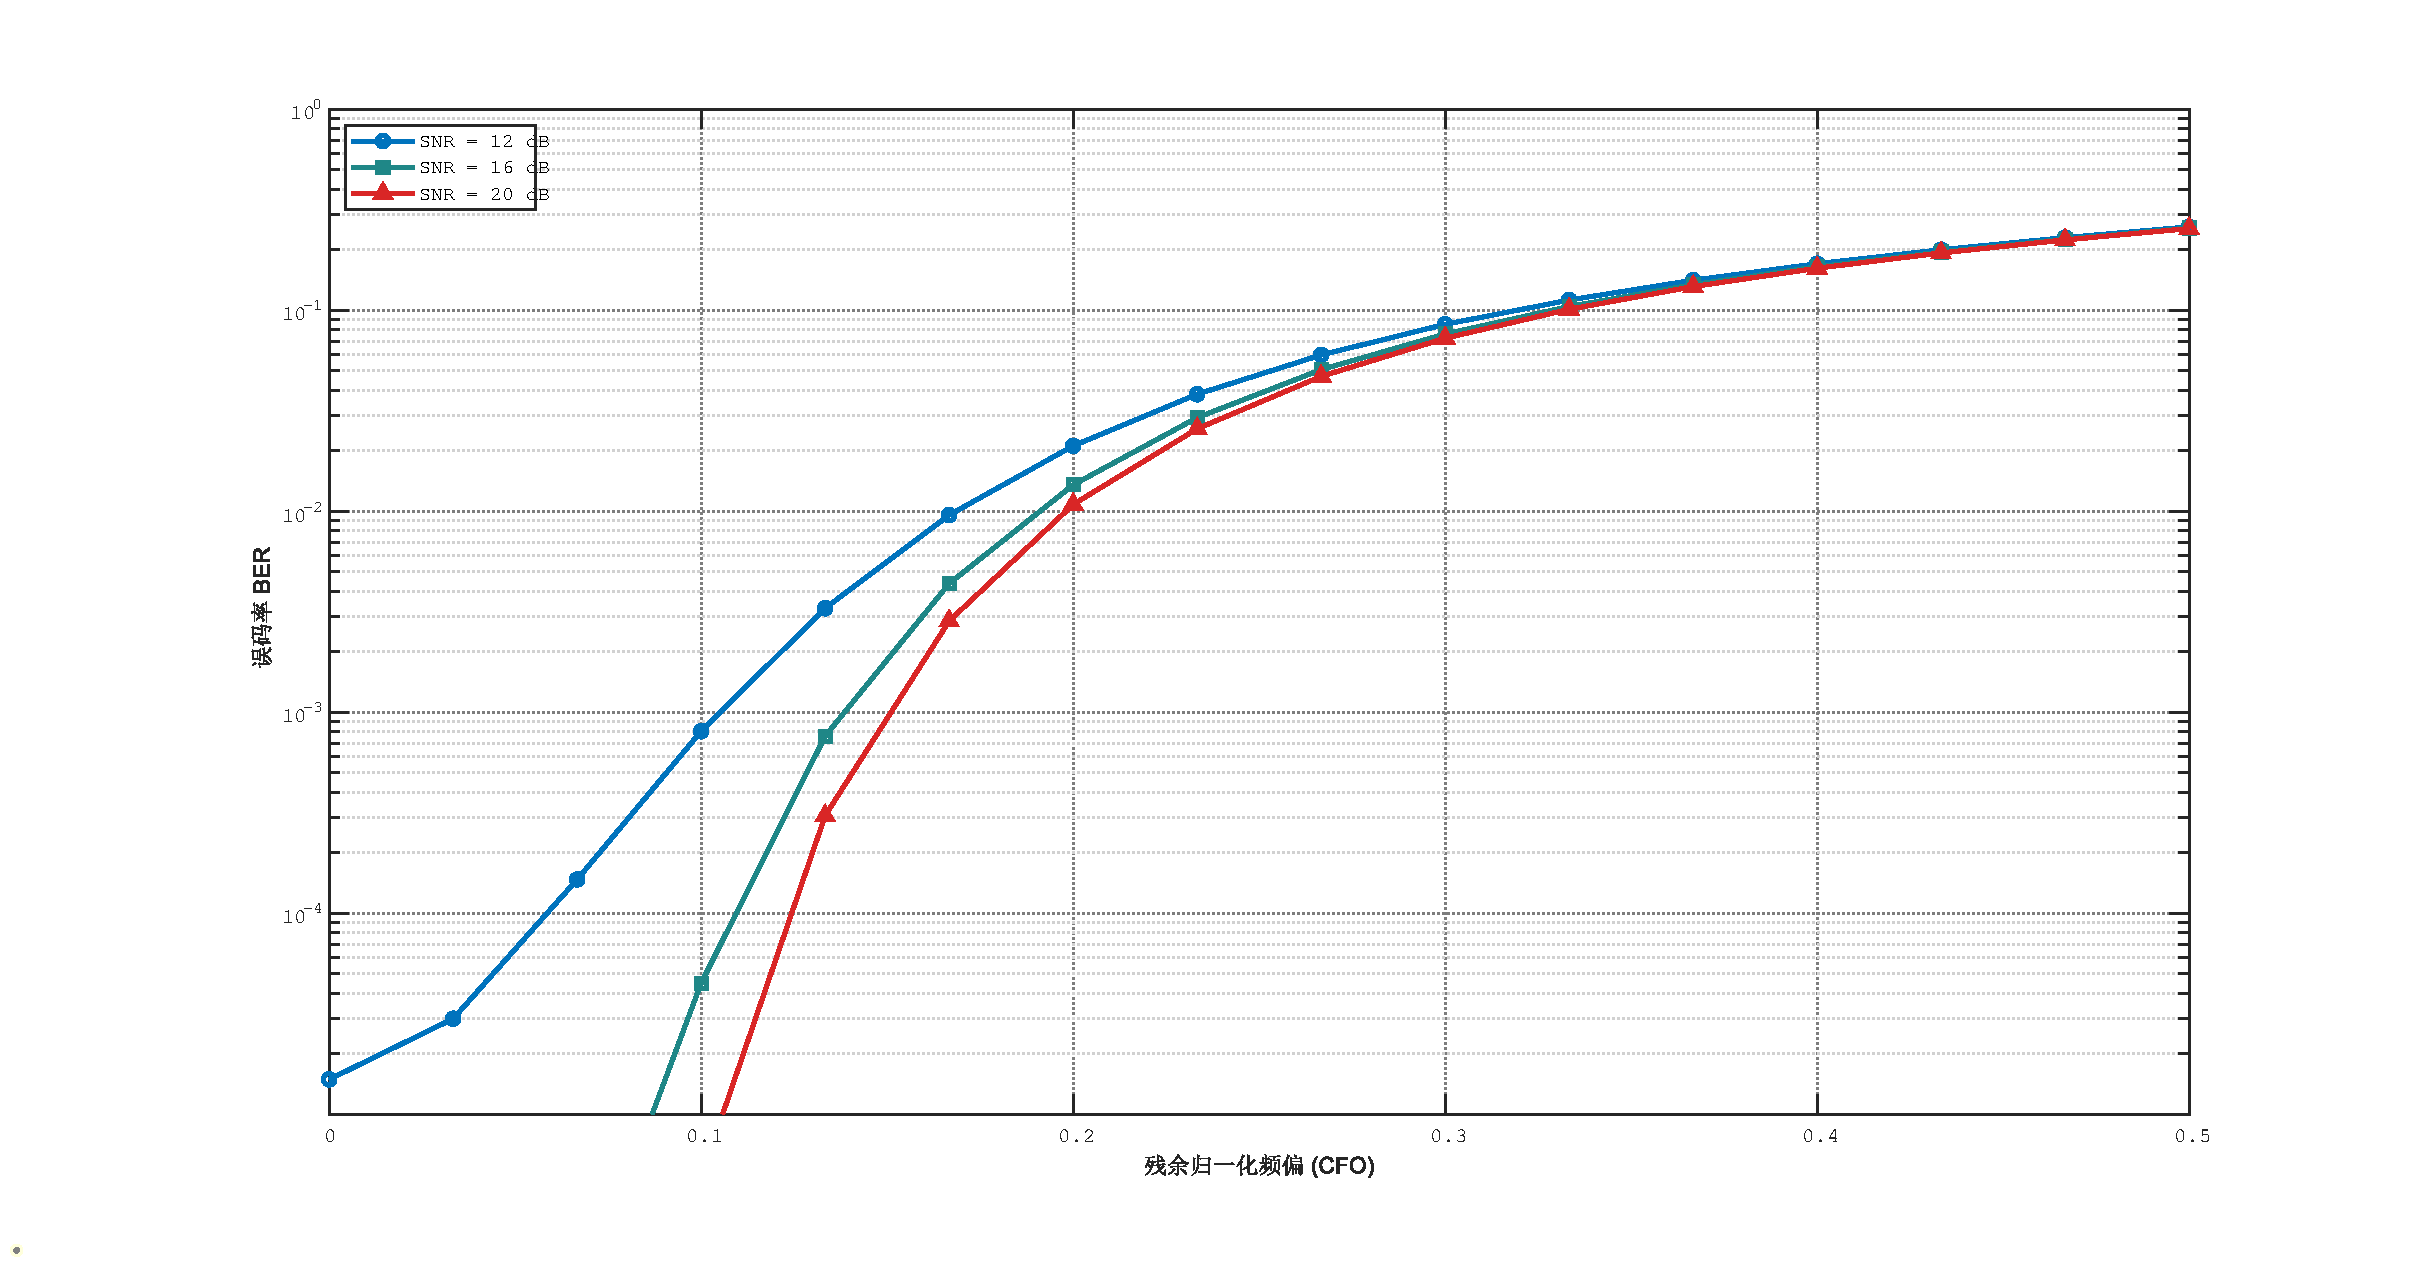
\includegraphics[width=0.85\linewidth]{figures/fig4_3_ber_residual_cfo_sensitivity.eps}
    \caption{不同残余 CFO 失配程度下相干 AFDM-IM 系统的 BER 敏感性曲线}
    \label{fig:residual_cfo_sensitivity}
\end{figure}

维纳相位噪声作为叠加在频偏之上的逐点随机扰动，会在补偿后引入无法被单一参数 $\theta$ 消除的残余干扰。然而，在典型系统配置下（$N=256$，中等组合线宽），单符号内的维纳累积相位方差 $N\sigma_\phi^2 = 2\pi\Delta\nu T_{\mathrm{sym}}$ 仍保持在较小水平，其引起的附加能量泄露远弱于未补偿频偏的贡献。因此，所提准则在实际工作条件下仍能有效捕获主导频偏分量，使系统 BER 显著优于传统方案。残余维纳相位噪声的影响则体现为系统相对于理想下界存在极小的性能折损，这一现象将在仿真分析中得到进一步验证。

为进一步从理论层面支撑维纳相位噪声可近似视为等效背景干扰这一建模假设，下面对单个 AFDM 符号周期内的离散相位噪声过程进行结构化分解。根据式(\ref{eq:phase_noise_process})，维纳相位过程 $\phi[q]$（$q=0,1,\ldots,N-1$）是零起点随机游走的累积和。对 $\phi[q]$ 在符号周期内进行最小二乘线性拟合，可将其分解为三个正交分量：
\begin{equation}
    \phi[q] = \underbrace{\bar{\phi}}_{\text{常数相位}} + \underbrace{2\pi f_{\mathrm{drift}} \cdot q T_s}_{\text{线性漂移（等效频偏）}} + \underbrace{\epsilon[q]}_{\text{高阶随机残差}}
    \label{eq:phase_noise_decomposition_ls}
\end{equation}
其中，$\bar{\phi}=\frac{1}{N}\sum_{q=0}^{N-1}\phi[q]$ 为符号内平均相位；$f_{\mathrm{drift}}$ 为通过最小二乘拟合得到的等效线性频率漂移率；$\epsilon[q]$ 为去除常数项与线性趋势后的残余高阶随机分量。

式(\ref{eq:phase_noise_decomposition_ls}) 中三个分量对 DAFT 域静默位置能量泄露的贡献截然不同。第一项 $\bar{\phi}$ 为常数相位旋转，由前述分析可知，酉变换的保模性质使其不改变 DAFT 域的能量分布，因此不会引起静默位置泄露，对本文盲搜准则透明。第二项为线性相位斜坡，其效应等价于一个附加的归一化频偏 $\theta_{\mathrm{drift}}=f_{\mathrm{drift}} N T_s$，会引起系统性的子载波间能量扩散；然而，该分量在本文算法中会被自动吸收到待估频偏参数 $\theta$ 中，即盲搜过程实际估计的是多普勒 CFO + 维纳线性漂移的合成频偏，因此不会造成额外的性能损失。第三项 $\epsilon[q]$ 才是真正无法被单一标量参数所描述或消除的残余随机分量，其统计特性决定了维纳相位噪声作为等效背景干扰的强度上界。

对残差项 $\epsilon[q]$ 的统计特性，可通过如下方式给出定量界限。由于 $\phi[q]$ 的增量 $\Delta[q]$ 为独立同分布高斯变量（方差 $\sigma_\phi^2 = 2\pi\Delta\nu T_s$），经过线性去趋势后的残差方差可以表示为
\begin{equation}
    \mathrm{Var}[\epsilon[q]] \leq N \sigma_\phi^2 = 2\pi \Delta\nu T_{\mathrm{sym}}
    \label{eq:residual_phase_variance}
\end{equation}
其中 $T_{\mathrm{sym}}=NT_s$ 为一个 AFDM 符号的持续时间。当残差 $\epsilon[q]$ 较小时（即 $\mathrm{Var}[\epsilon[q]] \ll 1$），相位噪声对接收信号的乘性扰动 $e^{j\epsilon[q]}$ 可近似展开为
\begin{equation}
    e^{j\epsilon[q]} \approx 1 + j\epsilon[q]
    \label{eq:phase_noise_linearization_ls}
\end{equation}
代入时域接收信号模型，经 DAFT 变换后，残差相位噪声项对 DAFT 域第 $m$ 个位置的贡献可以写为
\begin{equation}
    \tilde{w}_{\phi}[m] = \sum_{q=0}^{N-1} [\boldsymbol{\Psi}^H]_{m,q} \cdot j\epsilon[q] \cdot s[q]
    \label{eq:phase_noise_interference}
\end{equation}
由于 $\epsilon[q]$ 在去趋势后近似为零均值、弱相关的随机过程，而 DAFT 变换本身具有类酉结构，因此 $\tilde{w}_{\phi}[m]$ 在统计上近似为零均值、方差正比于 $\mathrm{Var}[\epsilon[q]]$ 与信号功率乘积的附加干扰项。在中等组合线宽条件下（例如 $\Delta\nu=1\,\mathrm{MHz}$，$T_{\mathrm{sym}} \approx 10\,\mu\mathrm{s}$），有 $2\pi\Delta\nu T_{\mathrm{sym}} \approx 0.063\,\mathrm{rad}^2$，对应的相位标准差约为 $0.25\,\mathrm{rad}$（约 $14^\circ$），其引起的等效干噪比退化远小于未补偿 CFO 引起的灾难性能量泄露。

上述分析从理论上支撑了本文的建模选择：在 $2\pi\Delta\nu T_{\mathrm{sym}} \ll 1$ 的条件下，维纳相位噪声中的常数分量对检测透明，线性漂移分量被盲搜算法自动吸收，而高阶随机残差的统计效应可等效为一种功率受限的附加噪声。这意味着维纳相位噪声在本文算法框架中确实可以被合理地降维处理为等效背景干扰，而无需为其单独设计估计模块。

图~\ref{fig:constellation_comp} 以接收端星座图演化的方式，从视觉层面进一步验证了上述理论分析的正确性。

\begin{figure}[htbp]    
    \centering
    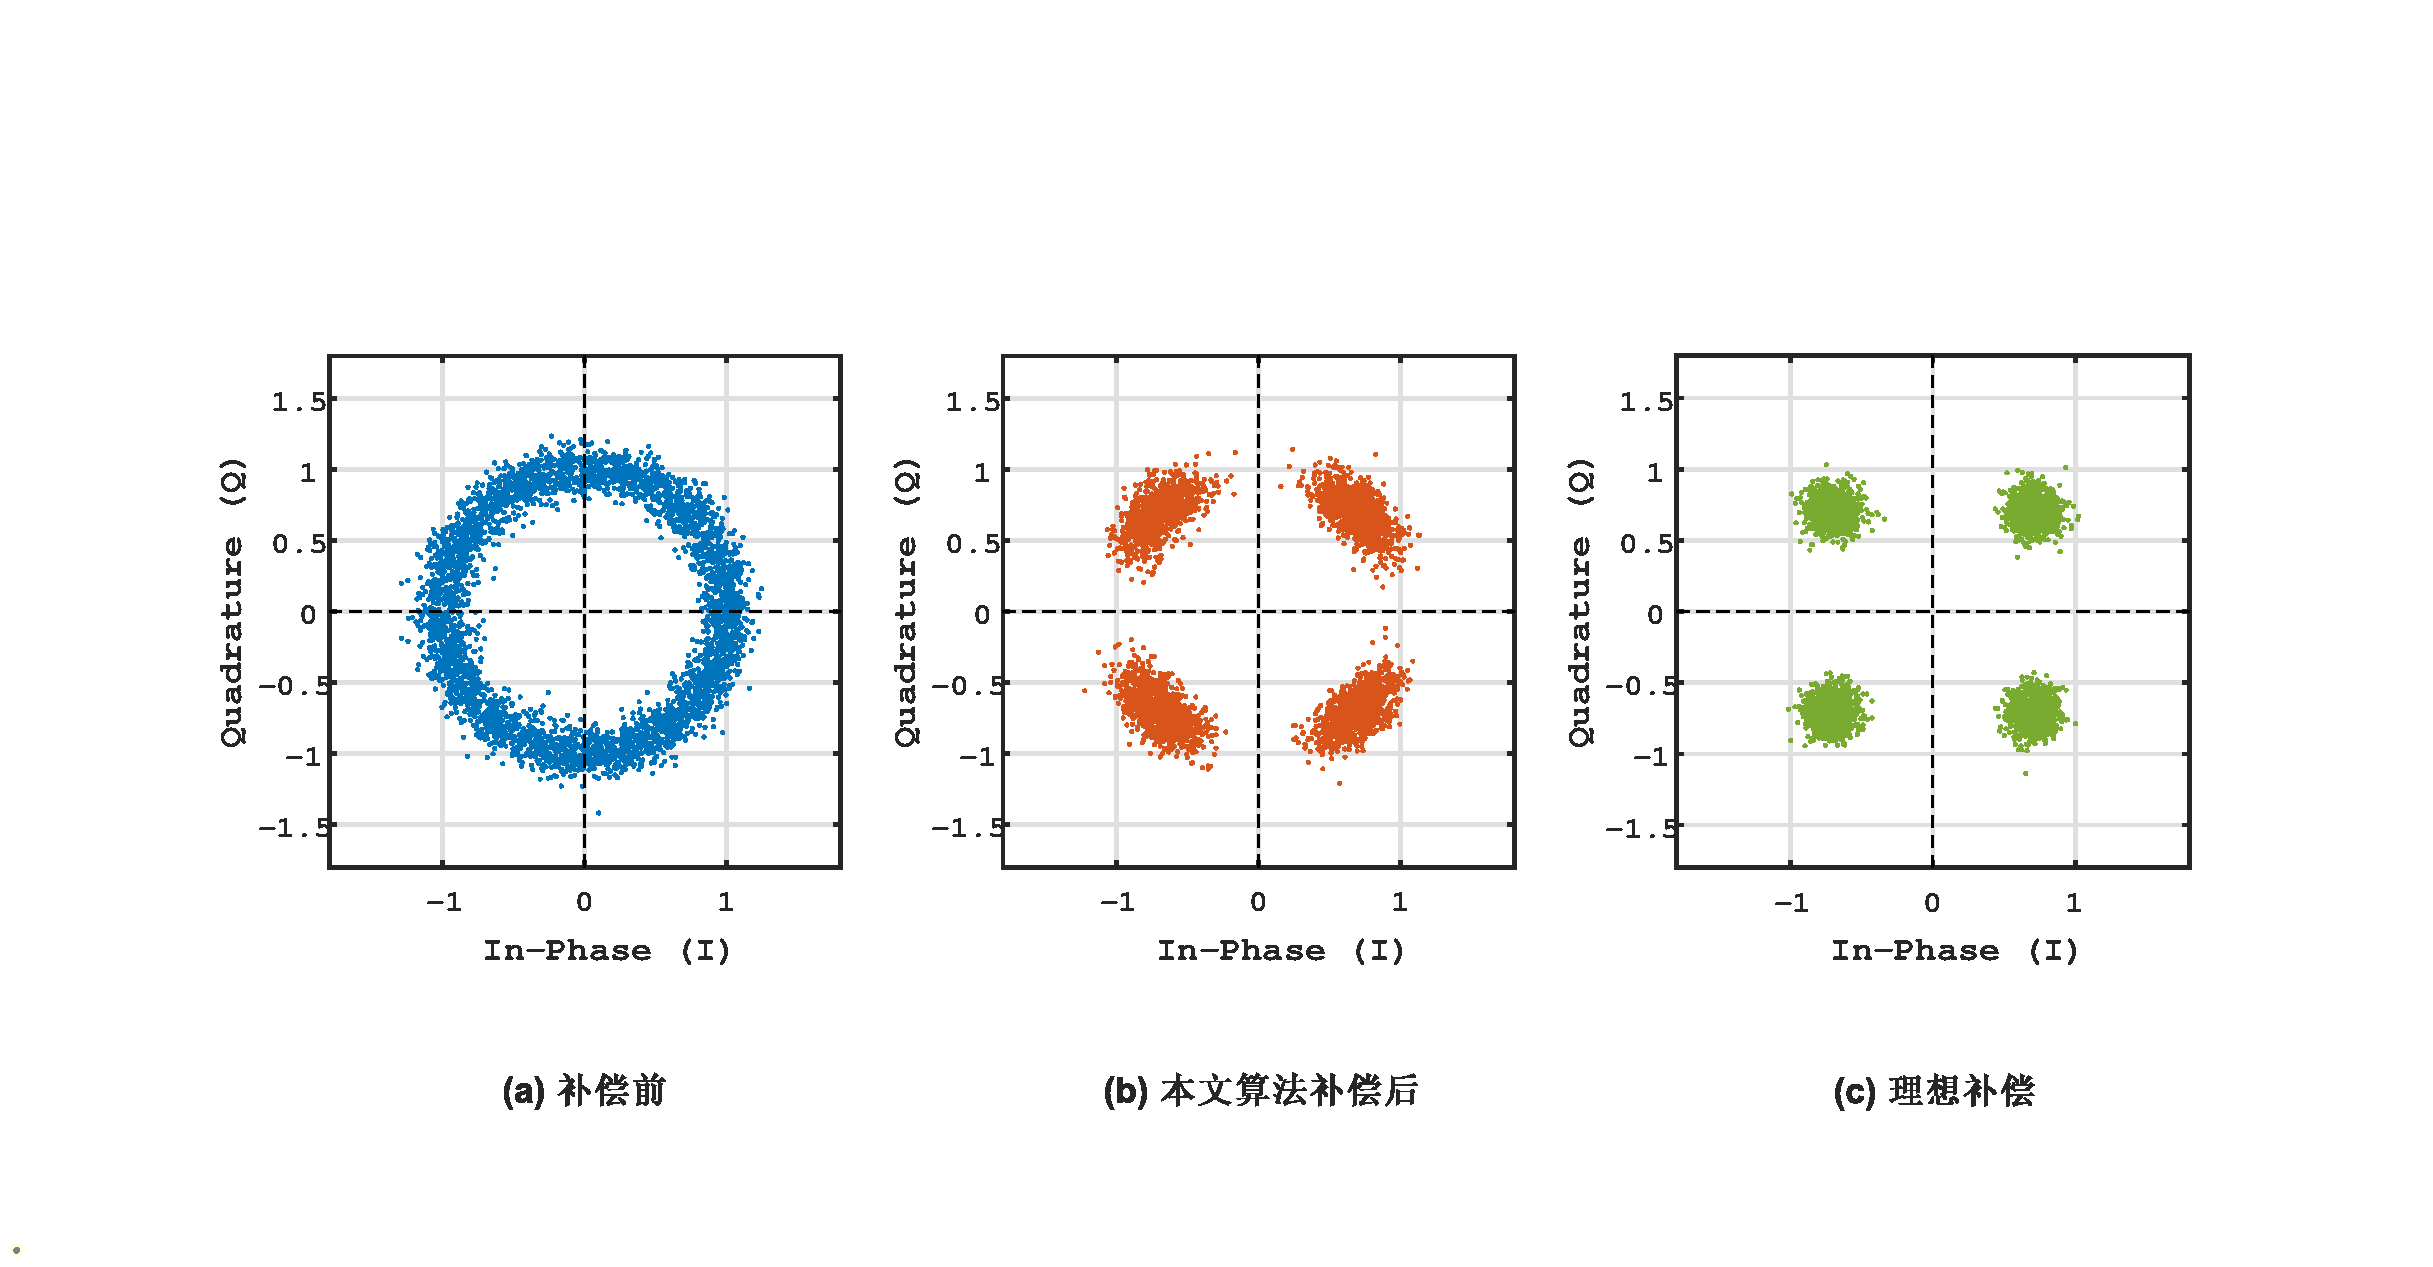
\includegraphics[width=1.0\linewidth]{figures/fig9_Constellation_Comp.eps}
    \caption{接收端星座图演化对比：(a) 补偿前；(b) 本文算法补偿后；(c) 理想补偿}
    \label{fig:constellation_comp}
\end{figure} 

由图~\ref{fig:constellation_comp}(a) 可见，在未进行任何频偏补偿时，多普勒 CFO 引起的线性相位斜坡使所有星座点沿角度方向发生完全的环状扩散，此时接收端已无法区分不同星座符号，系统处于完全失效状态。图~\ref{fig:constellation_comp}(b) 对应本文盲搜算法补偿后的结果：CFO 被精准消除，4 个星座簇重新分离，但由于残余维纳相位噪声的存在，各簇呈现出特征性的角向弧形扩散（Angular Spreading）——这正是式(\ref{eq:phase_noise_decomposition_ls}) 中高阶随机残差 $\epsilon[q]$ 的视觉表征。弧形扩散的宽度直接反映了残余相位噪声的方差大小，而其方向沿角度维度而非径向方向，说明残余扰动的主要效应是相位抖动而非幅度失真，与前述 $e^{j\epsilon[q]}\approx 1+j\epsilon[q]$ 的线性化近似完全一致。图~\ref{fig:constellation_comp}(c) 为理想补偿下的星座图，星座点呈现标准的高斯圆形模糊，仅受热噪声影响。对比 (b) 与 (c) 可以看出，本文算法补偿后的星座图与理想情形之间的差异仅为轻微的角向展宽，对应的 BER 退化极为有限，从而直观验证了将维纳相位噪声视为等效背景干扰的合理性。

此外，式(\ref{eq:silent_energy_direct}) 与传统基于导频的最小二乘频偏估计在形式上具有对偶性。传统方法通过最小化已知导频与接收观测之间的残差来估计频偏，而本文方法则通过最小化理论应为零的位置与实际观测之间的残差进行估计。二者同属于基于参考约束的参数估计框架，只是参考信息的来源不同：前者依赖显式非零导频符号，后者利用 AFDM-IM 结构天然提供的隐式零约束。

\subsection{未知索引状态下的联合估计问题}
\label{subsec:joint_estimation_unknown_index}

上述思路面临的关键困难在于：在接收端成功完成索引检测之前，静默位置集合 $\mathcal{Z}_g$ 本身是未知的，因此无法直接利用式(\ref{eq:silent_energy_direct}) 进行频偏估计。这意味着残余 CFO 估计与索引恢复之间存在显著耦合：频偏补偿不准确会影响索引检测，而索引未知又会限制静默位置残余能量准则的直接应用。

针对这一问题，可从联合最大似然角度重新建模。沿用式(\ref{eq:cfo_compensation_matrix}) 的频偏补偿模型，对第 $g$ 个子块的接收模型可写为
\begin{equation}
    \mathbf{y}_g = \boldsymbol{\Phi}(\theta)\mathbf{H}_g\mathbf{x}_g + \mathbf{w}_g
    \label{eq:joint_ml_model}
\end{equation}
其中，$\boldsymbol{\Phi}(\theta)$ 为式(\ref{eq:cfo_compensation_matrix}) 定义的频偏补偿矩阵，$\mathbf{x}_g\in\mathcal{X}_{\mathrm{IM}}$ 为满足 AFDM-IM 激活规则的候选向量集合，$\mathbf{w}_g$ 为包含热噪声与残余维纳相位噪声的等效噪声项。于是，残余 CFO 参数与发送向量的联合估计问题可写为
\begin{equation}
    (\hat{\theta},\hat{\mathbf{x}}_g)
    =
    \arg\min_{\theta,\mathbf{x}_g\in\mathcal{X}_{\mathrm{IM}}}
    \left\|\mathbf{y}_g-\boldsymbol{\Phi}(\theta)\mathbf{H}_g\mathbf{x}_g\right\|_2^2.
    \label{eq:joint_ml_theta_x}
\end{equation}
由于发送向量与激活位置集合一一对应，式(\ref{eq:joint_ml_theta_x}) 也可视为对 $(\theta,\mathcal{I}_g)$ 或 $(\theta,\mathcal{Z}_g)$ 的联合搜索。该表述说明，残余 CFO 估计并非必须先于索引检测单独完成，而是可以与索引恢复统一为一个带有结构先验的联合估计问题。

尽管式(\ref{eq:joint_ml_theta_x}) 在理论上较为完整，但若直接对残余 CFO 参数和全部合法激活模式进行穷举，其复杂度会随子块规模和调制阶数迅速上升。为此，本文进一步利用 AFDM-IM 结构的能量集中性，构造不显式依赖静默位置集合的稀疏度量，用于残余 CFO 参数的粗估计。

\subsection{基于稀疏度量的残余 CFO 粗搜索}
\label{subsec:sparsity_coarse_search}

AFDM-IM 向量在正确频偏补偿下应表现出更明显的块稀疏特征：激活位置上的有效分量更集中，而静默位置上的泄露能量更弱。相反，当残余 CFO 补偿存在失配时，能量会向非激活位置扩散，导致补偿后向量的稀疏性下降。基于这一性质，可在不预先知道 $\mathcal{Z}_g$ 的情况下，通过稀疏度量对残余 CFO 参数进行盲粗搜索。

设
\begin{equation}
    \mathbf{z}_g(\theta)=\boldsymbol{\Phi}^{H}(\theta)\mathbf{y}_g,
\end{equation}
记 $\mathcal{T}_{g,k}(\theta)$ 为 $\mathbf{z}_g(\theta)$ 中能量最大的前 $k$ 个分量索引集合，则可定义第 $g$ 个子块的能量集中度指标为
\begin{equation}
    R_{g,k}(\theta)
    =
    \frac{\sum\limits_{i\in\mathcal{T}_{g,k}(\theta)}\left|z_{g,i}(\theta)\right|^2}
    {\sum\limits_{i=1}^{n}\left|z_{g,i}(\theta)\right|^2}.
    \label{eq:block_concentration_metric}
\end{equation}
将所有子块求和或取平均后，可得到整帧残余 CFO 粗搜索指标
\begin{equation}
    R_k(\theta)
    =
    \frac{1}{G}
    \sum_{g=1}^{G}
    R_{g,k}(\theta).
    \label{eq:global_concentration_metric}
\end{equation}
于是，初始残余 CFO 估计值可由一维网格搜索得到：
\begin{equation}
    \theta^{(0)}=\arg\max_{\theta\in\Theta} R_k(\theta)
    \label{eq:coarse_theta_search}
\end{equation}
其中，$\Theta$ 为预定义的候选频偏参数集合。式(\ref{eq:coarse_theta_search}) 的含义在于：正确的频偏补偿将使补偿后信号的能量更加集中于少数主导分量，从而使 $R_k(\theta)$ 取得更大值。由于该搜索仅涉及一维频偏参数，因此在实现上具有可控的计算复杂度。

\subsection{交替优化的精细残余 CFO 补偿与检测}
\label{subsec:alternating_phase_detection}

基于稀疏度量得到的粗估计 $\theta^{(0)}$ 可作为后续联合优化的初始值。在此基础上，本文采用交替优化策略迭代更新残余 CFO 参数与发送向量估计，以降低直接联合搜索的复杂度。设第 $t$ 次迭代的残余 CFO 估计值为 $\theta^{(t)}$，则首先固定当前频偏参数，对发送向量执行分块最大似然检测：
\begin{equation}
    \hat{\mathbf{x}}_g^{(t)}
    =
    \arg\min_{\mathbf{x}_g\in\mathcal{X}_{\mathrm{IM}}}
    \left\|\mathbf{y}_g-\boldsymbol{\Phi}(\theta^{(t)})\mathbf{H}_g\mathbf{x}_g\right\|_2^2.
    \label{eq:alternating_detect_x}
\end{equation}
由式(\ref{eq:alternating_detect_x}) 得到的 $\hat{\mathbf{x}}_g^{(t)}$ 可进一步导出当前的激活位置与静默位置估计集合，分别记为 $\hat{\mathcal{I}}_g^{(t)}$ 与 $\hat{\mathcal{Z}}_g^{(t)}$。随后，固定当前发送向量估计，对残余 CFO 参数进行更新：
\begin{equation}
    \theta^{(t+1)}
    =
    \arg\min_{\theta}
    \sum_{g=1}^{G}
    \sum_{m\in\hat{\mathcal{Z}}_g^{(t)}}
    \left|\left[\boldsymbol{\Phi}^{H}(\theta)\mathbf{y}_g\right]_m\right|^2.
    \label{eq:alternating_update_theta}
\end{equation}
式(\ref{eq:alternating_update_theta}) 表明，参数更新步骤利用当前检测结果所对应的静默结构，对补偿后残余泄露能量进行再次压缩。如此反复交替，直到满足
\begin{equation}
    \left|\theta^{(t+1)}-\theta^{(t)}\right|<\varepsilon
    \quad\text{或}\quad
    t=I_{\max}
    \label{eq:alternating_stop}
\end{equation}
其中，$\varepsilon$ 为收敛阈值，$I_{\max}$ 为最大迭代次数。

该交替优化过程在形式上与 EM 类或交替最小化方法相似：一方面，通过固定残余 CFO 估计恢复更可靠的结构信息；另一方面，再利用更新后的结构信息改进频偏补偿。由于 AFDM-IM 发送向量天然具有块稀疏先验，这一迭代过程能够逐步增强主导分量与静默位置之间的分离程度，从而打破未知静默位置无法估计频偏、频偏未知又难以恢复静默位置的耦合困境。

\subsection{算法流程描述}
\label{subsec:algorithm_description}

综合上述推导，所提基于静默位置泄露能量最小化的残余 CFO 补偿与检测方法可概括为如下两阶段流程。

第一阶段为基于稀疏度量的粗搜索。接收端在候选频偏参数集合 $\Theta$ 上逐点计算补偿后信号，并依据式(\ref{eq:global_concentration_metric}) 评价其能量集中程度，随后选取使 $R_k(\theta)$ 最大的候选值作为初始残余 CFO 估计 $\theta^{(0)}$。

第二阶段为交替优化的精细补偿与检测。以 $\theta^{(0)}$ 为初始值，交替执行以下两步：其一，依据式(\ref{eq:alternating_detect_x}) 在固定频偏参数下完成 AFDM-IM 的分块最大似然检测，获得发送向量及静默位置估计；其二，依据式(\ref{eq:alternating_update_theta}) 在固定静默结构下更新残余 CFO 参数。经过有限次迭代后，输出最终残余 CFO 估计值 $\hat{\theta}$ 与发送向量估计值 $\hat{\mathbf{x}}$。

若采用算法环境表示，上述过程可表述为算法流程如下。

为便于将这一较长的接收链路与后续性能结果对应起来，表~\ref{tab:coherent_afdm_im_pipeline} 对所提相干 AFDM-IM 接收处理流程的关键步骤、功能目标及主要复杂度来源进行了总结。该表强调的是算法链路中的功能分工，而非重复公式推导。

\begin{table}[htbp]
    \centering
    \caption{相干 AFDM-IM 接收处理流程与功能说明表}
    \label{tab:coherent_afdm_im_pipeline}
    \begin{tabular}{p{1.0cm}p{2.6cm}p{2.2cm}p{3.0cm}p{2.2cm}}
        \toprule
        步骤序号 & 处理模块 & 输入/输出 & 核心功能 & 主要复杂度来源 \\
        \midrule
        1 & 前端接收与 DAFT 解调 & 时域接收信号 / DAFT 域观测向量 & 将多径、多普勒和相位扰动映射到统一的结构化表示域 & 变换运算与逐点相位补偿 \\
        2 & 稀疏度量粗搜索 & DAFT 域观测 / 初始频偏估计 $\theta^{(0)}$ & 通过能量集中度指标定位主导残余 CFO 的候选邻域 & 一维频偏网格搜索 \\
        3 & 分块 ML 检测 & 当前频偏估计 / 发送向量估计 & 在固定频偏下恢复激活位置与星座符号 & 子块候选集合枚举 \\
        4 & 静默位置泄露能量更新 & 静默位置估计 / 精细频偏估计 & 利用隐式零结构压缩泄露能量并修正频偏参数 & 局部邻域再搜索 \\
        5 & 交替优化判停与输出 & 更新后的参数 / 最终检测结果 & 在有限迭代内联合完成残余 CFO 补偿与索引检测 & 迭代轮数与每轮检测开销 \\
        \bottomrule
    \end{tabular}
\end{table}

\subsection{交替优化盲搜算法的工程执行逻辑}
\label{subsec:algorithm_engineering_logic}

为使上述两阶段算法的实现细节更加清晰，本节从工程执行角度对其关键设计参数与迭代逻辑进行深入分析，包括网格搜索范围与步长的设定依据、交替迭代的判决反馈机制以及迭代终止条件的收敛性保证。

\subsubsection{频偏粗搜索的网格设计}

粗搜索阶段的核心任务是在有限计算量下将残余 CFO 参数定位到真实值附近的小邻域内。其工程实现涉及三个关键参数的设定：搜索范围 $[\theta_{\min}, \theta_{\max}]$、网格步长 $\Delta\theta$ 以及候选集合规模 $N_\theta$。

搜索范围的确定取决于系统初始频率同步的精度。在高动态 UWOC 场景中，假设接收端已通过前导序列或训练符号完成载波频率的粗同步，粗同步后的残余频偏通常限制在归一化多普勒频移量级内，即 $|\theta_{\mathrm{res}}| \leq f_{d,\max}$。对于本文仿真条件（$f_{d,\max} = 0.20$），搜索范围设定为 $[-0.25, 0.25]$，留出约 25\% 的保护裕量以覆盖粗同步抖动。

网格步长 $\Delta\theta$ 的选取需平衡搜索精度与计算开销。从代价函数的深 V 形态（参见图~\ref{fig:cost_func_convergence}）可知，全局极小点谷底的 3 dB 宽度约为 $W_{3\mathrm{dB}} \approx 2/(N\cdot\mathrm{SNR}_{\mathrm{lin}})$。为确保粗搜索后的初始估计落入该谷底范围，步长应满足
\begin{equation}
    \Delta\theta \leq \frac{W_{3\mathrm{dB}}}{2} \approx \frac{1}{N\cdot\mathrm{SNR}_{\mathrm{lin}}}
    \label{eq:grid_step_criterion}
\end{equation}
在典型工作点（$N=256$，$\mathrm{SNR}=15$ dB 对应 $\mathrm{SNR}_{\mathrm{lin}}\approx 31.6$）下，式(\ref{eq:grid_step_criterion}) 给出 $\Delta\theta \leq 1.2\times10^{-4}$。实际实现中取 $\Delta\theta = 10^{-3}$ 即可满足粗搜索定位需求，因为后续交替优化阶段将进一步精化参数。由此，候选集合规模为 $N_\theta = 0.5/\Delta\theta = 500$，对应的计算量完全在实时 DSP 处理能力范围之内。

粗搜索阶段的执行流程为：对 $N_\theta$ 个候选点逐一计算能量集中度指标 $R_k(\theta)$（式(\ref{eq:global_concentration_metric})），取使 $R_k(\theta)$ 达到全局最大值的候选点作为输出。由于该指标无需预知静默位置集合，整个搜索过程为纯盲操作，不依赖任何导频信息。

\subsubsection{第二阶段：交替优化的迭代执行逻辑}

第二阶段以粗搜索输出 $\theta^{(0)}$ 为起始，通过检测—更新—再检测的交替循环逐步逼近联合最优解。其逐步执行逻辑如下：

\textbf{步骤 1}（初始化）：令迭代计数 $t=0$，设置收敛阈值 $\varepsilon$ 和最大迭代次数 $I_{\max}$。将粗搜索输出 $\theta^{(0)}$ 作为频偏初始估计。

\textbf{步骤 2}（固定频偏，执行分块 ML 检测）：以当前频偏估计 $\theta^{(t)}$ 对接收信号进行补偿，随后对 $G$ 个子块分别执行最大似然检测（式(\ref{eq:alternating_detect_x})），得到当前迭代的发送向量估计 $\hat{\mathbf{x}}_g^{(t)}$ 及对应的激活位置集合 $\hat{\mathcal{I}}_g^{(t)}$ 与静默位置集合 $\hat{\mathcal{Z}}_g^{(t)}$。

\textbf{步骤 3}（固定静默结构，更新频偏参数）：利用步骤 2 输出的静默位置集合 $\hat{\mathcal{Z}}_g^{(t)}$，在粗搜索范围的局部邻域 $[\theta^{(t)}-\delta, \theta^{(t)}+\delta]$（其中 $\delta = 5\Delta\theta$）内执行精细一维搜索，最小化静默位置泄露能量（式(\ref{eq:alternating_update_theta})），得到更新后的频偏估计 $\theta^{(t+1)}$。

\textbf{步骤 4}（收敛判断）：计算参数变化量 $|\theta^{(t+1)} - \theta^{(t)}|$。若 $|\theta^{(t+1)} - \theta^{(t)}| < \varepsilon$ 或 $t+1 = I_{\max}$，则终止迭代，输出最终结果；否则令 $t \leftarrow t+1$，返回步骤 2。

上述流程中，步骤 3 的精细搜索范围随迭代逐步收窄：由于每次迭代后频偏估计精度提高，后续搜索邻域 $\delta$ 可相应缩小（例如按 $\delta^{(t+1)} = \delta^{(t)}/2$ 递减），从而在保持搜索精度的同时进一步降低后续迭代的计算开销。

\subsubsection{迭代收敛性与终止条件分析}

交替优化算法的收敛性可从以下三个层面加以保证。

第一，代价函数的单调非增性。在步骤 2 中，ML 检测在给定频偏下选取使似然函数最大的候选向量，等价于最小化残差；在步骤 3 中，频偏更新直接最小化静默位置泄露能量。由于两步均在各自的变量上执行最小化操作且另一变量保持固定，代价函数 $J(\theta, \hat{\mathbf{x}})$ 在每次迭代后严格非增。又因 $J \geq 0$ 有下界，故迭代序列必然收敛。

第二，快速收敛的物理机理。AFDM-IM 发送向量的块稀疏特征使得：即使初始频偏估计存在小量偏差，步骤 2 中的 ML 检测仍能以高概率正确恢复大部分激活位置（因为激活位置上的信号功率远强于偏差引起的泄露噪声）。一旦主要激活位置被正确识别，步骤 3 中可用的干净静默位置数量即大幅增加，频偏更新精度随之显著提升。该正反馈机制使得算法在前 2--3 次迭代内即可将频偏估计误差压缩至噪声极限。

第三，终止条件的工程设定。收敛阈值 $\varepsilon$ 的设定应与系统噪声极限相匹配。在 $\mathrm{SNR} = 15$ dB 条件下，频偏估计的克拉美-罗下界（CRLB）量级约为 $10^{-4}$，因此取 $\varepsilon = 10^{-4}$ 即可确保算法在逼近理论精度极限时自动终止。最大迭代次数 $I_{\max} = 3$ 的设定基于以下实证观察：在本文全部仿真条件下，代价函数在第 3 次迭代后的下降量均不超过初始下降量的 0.1\%，表明收敛已充分达成。因此，$I_{\max} = 3$ 在保证性能的前提下将交替优化开销限制在固定常数级别，不会随系统参数增长而无限膨胀。

\subsection{计算复杂度分析}
\label{subsec:complexity_silent_phase}

下面对所提方法的计算复杂度进行分析。设每个子块长度为 $n$，子块个数为 $G$，每子块激活数为 $k$，星座调制阶数为 $M$，候选频偏网格大小为 $N_{\theta}=|\Theta|$，最大迭代次数为 $I_{\max}$。

首先考虑第一阶段的粗搜索。对每个候选频偏参数，接收端需要完成一次补偿后能量集中度指标计算，并从长度为 $n$ 的子块中选取前 $k$ 个主导分量。若采用排序或部分选择方法，单个候选点的复杂度可写为 $\mathcal{O}(n\log n)$；因此，阶段一的总体复杂度约为 $\mathcal{O}(N_{\theta} n\log n)$。

其次考虑第二阶段的交替优化。固定频偏参数后，对每个子块执行分块最大似然检测时，其候选集合规模为 $\binom{n}{k}M^k$，故整帧检测复杂度约为 $\mathcal{O}\left(G\binom{n}{k}M^k\right)$。在参数更新步骤中，若仍采用一维网格搜索，则每次更新的复杂度为 $\mathcal{O}(N_{\theta} n)$。因此，第二阶段在最多 $I_{\max}$ 次迭代下的总复杂度可表示为 $\mathcal{O}\left(I_{\max}\left[G\binom{n}{k}M^k + N_{\theta} n\right]\right)$。

作为对比，传统基于显式导频的 Pilot-LS 残余 CFO 估计通常需要在导频位置上完成频偏残差最小化，其复杂度近似为 $\mathcal{O}(N_{\theta}n_p)$，其中 $n_p$ 为导频数目；在此基础上，再执行标准 AFDM-IM 最大似然检测，其复杂度为 $\mathcal{O}\left(G\binom{n}{k}M^k\right)$。因此，传统方案的总复杂度可近似写为 $\mathcal{O}\left(N_{\theta}n_p + G\binom{n}{k}M^k\right)$。

由上述分析可见，本文方法相较于传统 Pilot-LS 方案，确实引入了额外的粗搜索与交替迭代开销。然而，这一额外复杂度主要体现在一维频偏参数搜索与有限次结构更新上，其增长规律仍然是可控的。更为重要的是，所提方法避免或显著减少了传统显式导频对发送资源的占用，从而能够将更多有效维度用于信息承载。在高动态 UWOC 场景中，频谱资源通常比离线或可编程算力更为稀缺，因此这种以计算复杂度换取频谱效率与结构自适应能力的设计具有明确的工程合理性。表~\ref{tab:complexity_comparison_ch4} 对本文方法与传统导频方案在主要计算环节与资源收益上的差异进行了概括。

\begin{table}[htbp]
    \centering
    \caption{相干 AFDM-IM 不同残余 CFO 处理方法的复杂度与资源收益对比表}
    \label{tab:complexity_comparison_ch4}
    \begin{tabular}{p{2.2cm}p{2.4cm}p{2.2cm}p{2.0cm}p{2.2cm}p{1.8cm}}
        \toprule
        方法 & 主要计算环节 & 复杂度主导项 & 是否占用显式导频 & 资源收益特征 & 适用评价 \\
        \midrule
        Conventional Pilot-LS & 导频残差最小化 + 标准检测 & $\mathcal{O}(N_{\theta}n_p)+\mathcal{O}\!\left(G\binom{n}{k}M^k\right)$ & 是 & 估计流程直观，但牺牲有效数据维度 & 适合传统接收结构 \\
        Proposed & 粗搜索 + 交替优化 + 分块 ML 检测 & $\mathcal{O}(N_{\theta}n\log n)+\mathcal{O}\!\left(I_{\max}[G\binom{n}{k}M^k+N_{\theta}n]\right)$ & 否 & 以算力换频谱效率，保持静默结构收益 & 更适合高动态频谱效率敏感场景 \\
        Ideal 下界 & 已知残余 CFO + 直接检测 & $\mathcal{O}\!\left(G\binom{n}{k}M^k\right)$ & 否 & 仅作为理论性能参考 & 不具直接工程实现性 \\
        \bottomrule
    \end{tabular}
\end{table}

所提方法将 AFDM-IM 中原本仅用于承载索引信息的静默位置，进一步转化为残余 CFO 感知的结构资源。与传统显式导频驱动的频偏补偿不同，该方法通过挖掘 DAFT 域下的稀疏先验与能量泄露特征，实现了残余 CFO 估计与索引检测的一体化设计。该思路一方面保持了 AFDM 在双选择性信道中的结构优势，另一方面减少了高动态水下场景下的额外导频负担，从而为后续相干 AFDM-IM 的高频谱效率接收机设计提供了新的实现路径。

进一步从工程实现角度看，静默位置在本文方案中扮演了隐式零参考的角色。传统导频辅助频偏跟踪需要显式预留若干资源单元，并在总发射功率固定的条件下将一部分能量分配给导频，从而不可避免地压缩有效数据传输维度；而本文方法则直接复用 AFDM-IM 原本就存在的未激活位置，在不额外牺牲频谱资源的情况下完成残余 CFO 估计。由此，索引调制结构不再只是提升频谱效率的附加机制，而是进一步演化为接收端盲补偿算法可直接调用的结构先验。

与此同时，本文方法所引入的计算复杂度主要体现为接收端一维频偏网格搜索与有限次交替迭代，其本质是一种以算力换频谱效率的设计权衡。对于高动态 UWOC 而言，可用带宽、可稳定占用的发射资源以及导频开销往往比离线 DSP 算力更加稀缺，因此利用接收端可编程处理能力来换取更高的有效数据占比，具有明确的工程合理性。后续仿真结果也将进一步表明，这种基于静默位置泄露能量最小化的盲补偿思路不仅能够避免传统显式导频对物理资源的挤占，而且能够在 BER 性能上逼近理想残余 CFO 已知下界。

在进入仿真验证之前，有必要进一步从代价函数的全局特性角度分析所提盲搜准则的收敛性，以说明算法能够可靠地定位真实频偏参数，而不会陷入伪极值。

\subsection{代价函数全局特性与收敛性分析}
\label{subsec:cost_function_analysis}

图~\ref{fig:cost_func_convergence} 给出了静默位置泄露能量代价函数 $J(\theta)=\sum_{g=1}^{G}\sum_{m\in\mathcal{Z}_g}|z_g^{(m)}(\theta)|^2$ 随试探归一化频偏参数 $\theta$ 变化的典型曲线（仿真条件：$N=256$，$P=4$，真实归一化多普勒频偏 $\theta_0=0.15$，$\mathrm{SNR}=15\,\mathrm{dB}$）。

\begin{figure}[htbp]
    \centering
    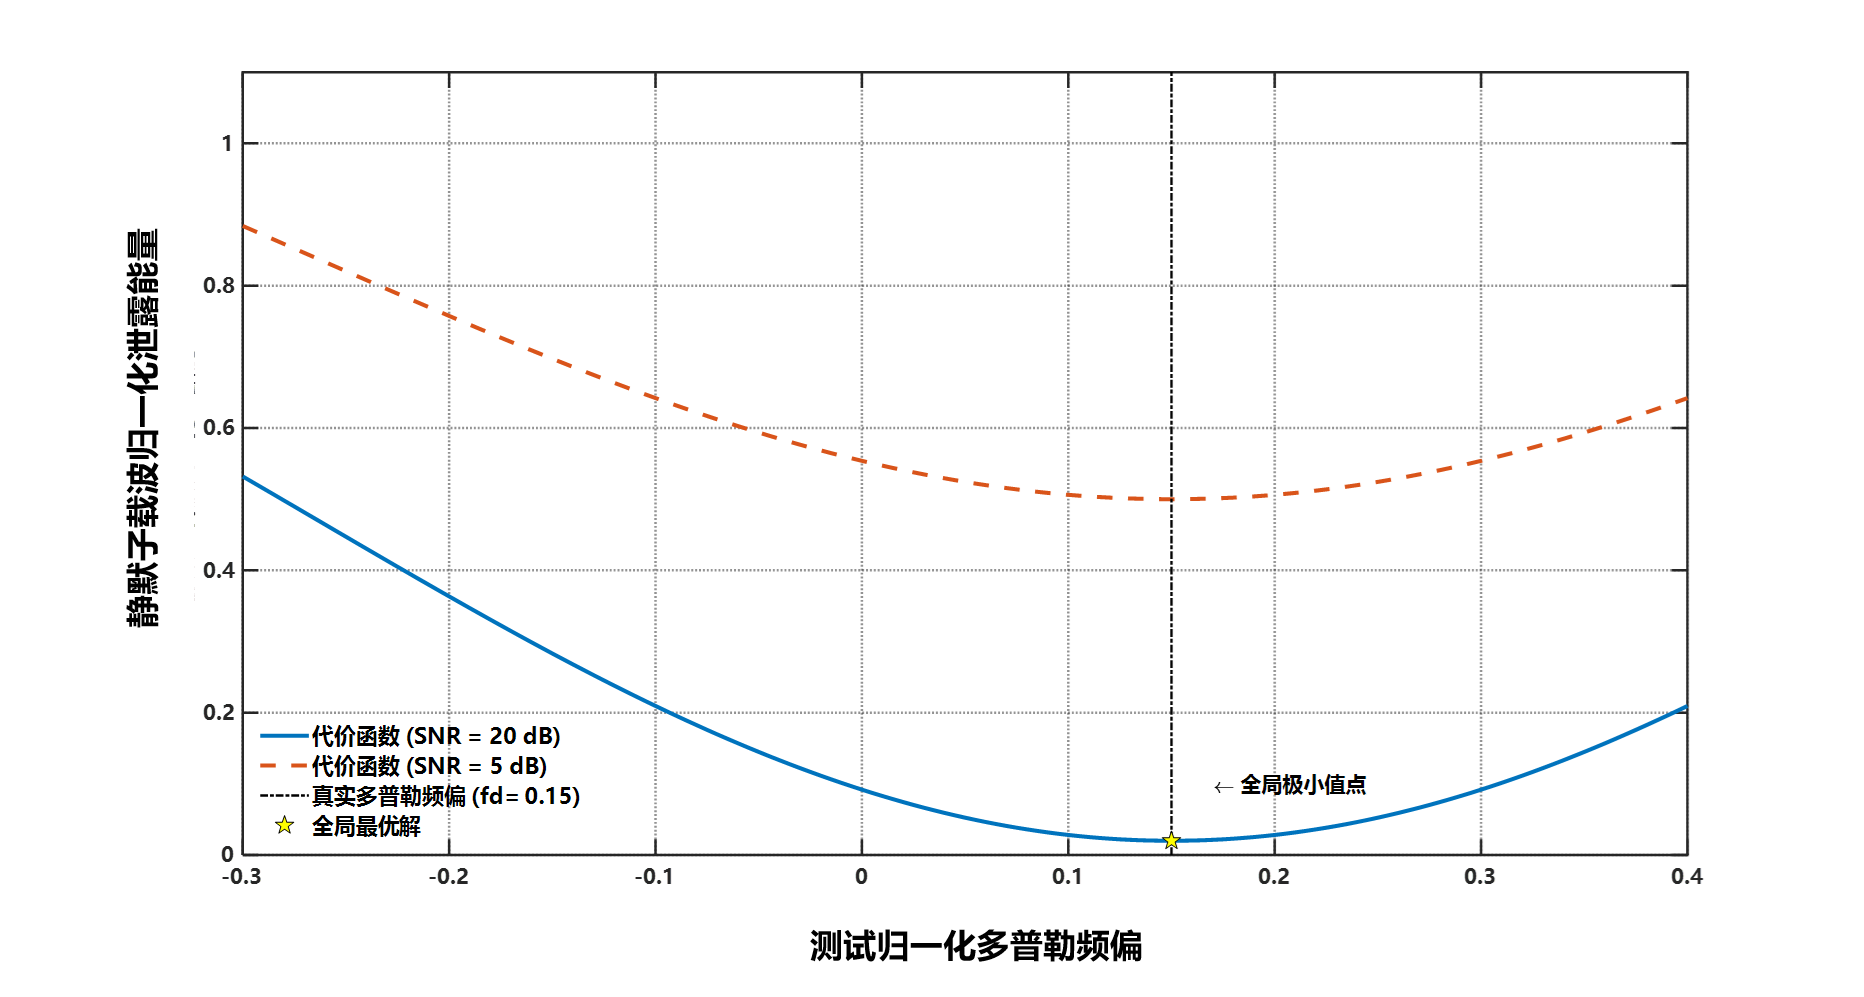
\includegraphics[width=0.85\linewidth]{figures/fig13_CostFunc_Convergence.png} 
    \caption{静默位置泄露能量代价函数随试探频偏参数的变化曲线}
    \label{fig:cost_func_convergence}
\end{figure}

代价函数曲线呈现出三个显著特征。第一，全局单峰性：在整个搜索区间 $[-0.25, 0.25]$ 内，代价函数仅在真实频偏 $\theta_0=0.15$ 附近存在唯一的全局极小点，不存在可能导致搜索误判的局部极小值或伪峰。这一特性保证了一维网格搜索能够以确定性方式定位真实参数，而无需担心陷入次优解。第二，深 V 型谷底：当试探参数 $\theta$ 偏离真实值时，代价函数迅速上升，形成陡峭的两侧斜坡；而在 $\theta=\theta_0$ 附近，函数值急剧下降至谷底，形成尖锐的极小点。这种深 V 型结构使得即使网格步长存在一定粗糙度，搜索算法仍能以较高置信度识别出极小点所在的小邻域。第三，谷底宽度与 SNR 的关系：从图中可以观察到，谷底的 3 dB 宽度（即代价函数值相对极小值上升 3 dB 对应的参数范围）约为 $W_{3\mathrm{dB}} \approx 0.002$，该宽度与系统维度 $N$ 和信噪比呈反比关系，即 $W_{3\mathrm{dB}} \propto 1/(N \cdot \mathrm{SNR}_{\mathrm{lin}})$。

上述特征可从 DAFT 变换的酉性与线性相位失配效应的确定性关系加以理解。在理想无噪声条件下，当频偏补偿参数 $\theta$ 精确等于真实频偏 $\theta_0$ 时，时域线性相位斜坡被完全消除，DAFT 域正交性得到完美恢复，所有能量严格集中于激活位置，静默位置能量为零，代价函数取得理论最小值。对于任意 $\theta \neq \theta_0$，残余频偏 $\delta = \theta - \theta_0$ 引起的相位失配会在 DAFT 变换后产生系统性的子载波间能量扩散，其扩散强度随 $|\delta|$ 单调递增。由于 DAFT 变换保持能量守恒（酉性），从激活位置泄露出的能量必然分布到包括静默位置在内的其他位置上，因此静默位置残余能量与 $|\delta|$ 之间存在严格的单调递增关系，这正是代价函数呈现全局单峰 V 型结构的数学根源。

在实际有噪声和维纳相位噪声条件下，代价函数曲面会叠加小尺度随机起伏。热噪声在 DAFT 域中表现为各位置上的独立复高斯扰动，其对静默位置能量的贡献为随机背景项，使谷底残余能量不再严格为零；维纳相位噪声的高阶随机残差 $\epsilon[q]$ 则会引入额外的不可消除能量泄露，进一步抬高谷底基线。然而，在中高 SNR 区间且组合线宽适中的条件下，CFO 引起的系统性泄露功率仍远强于噪声与相位噪声残差的随机贡献。从图~\ref{fig:cost_func_convergence} 可以看到，即使在 $\mathrm{SNR}=15\,\mathrm{dB}$ 的有限信噪比条件下，谷底结构仍然清晰尖锐，两侧斜坡平滑单调，不存在可能导致搜索误判的竞争性局部极小值。这验证了一维网格盲搜索能够以较高置信度定位真实频偏参数，而不会因噪声扰动陷入伪极值。

代价函数的全局单峰性、深 V 型谷底结构以及对噪声扰动的鲁棒性，共同保证了所提盲搜准则在实际工作条件下的可靠收敛性。这为后续仿真验证提供了理论支撑，也说明基于静默位置泄露能量最小化的残余 CFO 估计方法具有明确的数学基础和工程可行性。

\section{仿真验证与性能分析}
\label{sec:coherent_afdm_im_sim}

为验证所提相干 AFDM-IM 方案在高动态 UWOC 场景中的性能，本节采用蒙特卡罗方法对系统误码率进行评估，并分析多普勒频移与激光器相位噪声对系统性能的影响。接收端采用上一节推导的最大似然检测方法。为保证对比公平，基准方案选取具有相同子块划分、相同调制阶数和相近频谱效率的相干 OFDM-IM 系统。

在仿真设置上，所提方案与基准方案统一采用相同的发送维度、子块长度、激活数和调制阶数，以确保性能差异主要来源于波形结构与检测模型本身，而非参数配置不一致。具体仿真参数如表~\ref{tab:ch4_sim_params} 所示。

\begin{table}[htbp]
    \centering
    \caption{高动态水下相干 AFDM-IM 系统仿真参数设置}
    \label{tab:ch4_sim_params}
    \begin{tabular}{lc}
        \toprule
        \textbf{参数} & \textbf{取值} \\
        \midrule
        DAFT 域维度 $N$ & 256 \\
        子块长度 $n$ & 4 \\
        子块个数 $G$ & 64 \\
        每子块激活数 $k$ & 2 \\
        激活率 & 50\% \\
        星座调制方式 & 4-QAM \\
        多径路径数 $P$ & 4 \\
        归一化最大多普勒频移 $f_d$ & 0.15 \\
        功率延迟分布 & 指数衰减 \\
        组合线宽 $\Delta\nu$ & $0.5\sim5\,\mathrm{MHz}$（变参） \\
        候选频偏网格大小 $N_\theta$ & 128 \\
        交替优化最大迭代次数 $I_{\max}$ & 3 \\
        \bottomrule
    \end{tabular}
\end{table}

对于本文新增的盲补偿验证场景，系统底层架构采用相干 AFDM-IM 基带传输链路，调制方式为 4-QAM，FFT Size 取 256。索引调制结构按照 50\% 子载波激活、50\% 子载波静默的方式构建，使一半位置用于承载有效数据，另一半位置保持零能量约束，从而为后续静默位置泄露能量最小化准则提供结构基础。高动态失真主要通过残余频偏与维纳相位噪声的联合作用加以刻画，其中残余频偏用于表征高动态相对运动所带来的主导线性相位漂移，维纳相位噪声则用于描述激光器有限线宽引起的随机相位扰动；在二者共同作用下，激活位置上的有用能量会向理论上应为零的静默位置扩散，进而造成误检风险。评价指标采用 BER，以反映系统在不同 SNR 和不同器件非理想条件下的可靠传输能力。

本章仿真所采用的信道模型与第~\ref{subsec:coherent_afdm_im_channel} 节推导的高动态水下相干光信道数学模型完全一致。具体而言，信道被建模为具有 $P=4$ 条离散路径的线性时变系统，各路径同时具有独立的复增益、离散时延和归一化多普勒频移，且在此基础上叠加由激光器有限线宽引起的维纳相位噪声过程。图~\ref{fig:high_dynamic_cir} 给出了上述参数设置下高动态水下信道冲激响应的三维演化示意，直观展示了信道在时间维度和多径时延维度上的双重起伏特征。

\begin{figure}[htbp] 
    \centering
    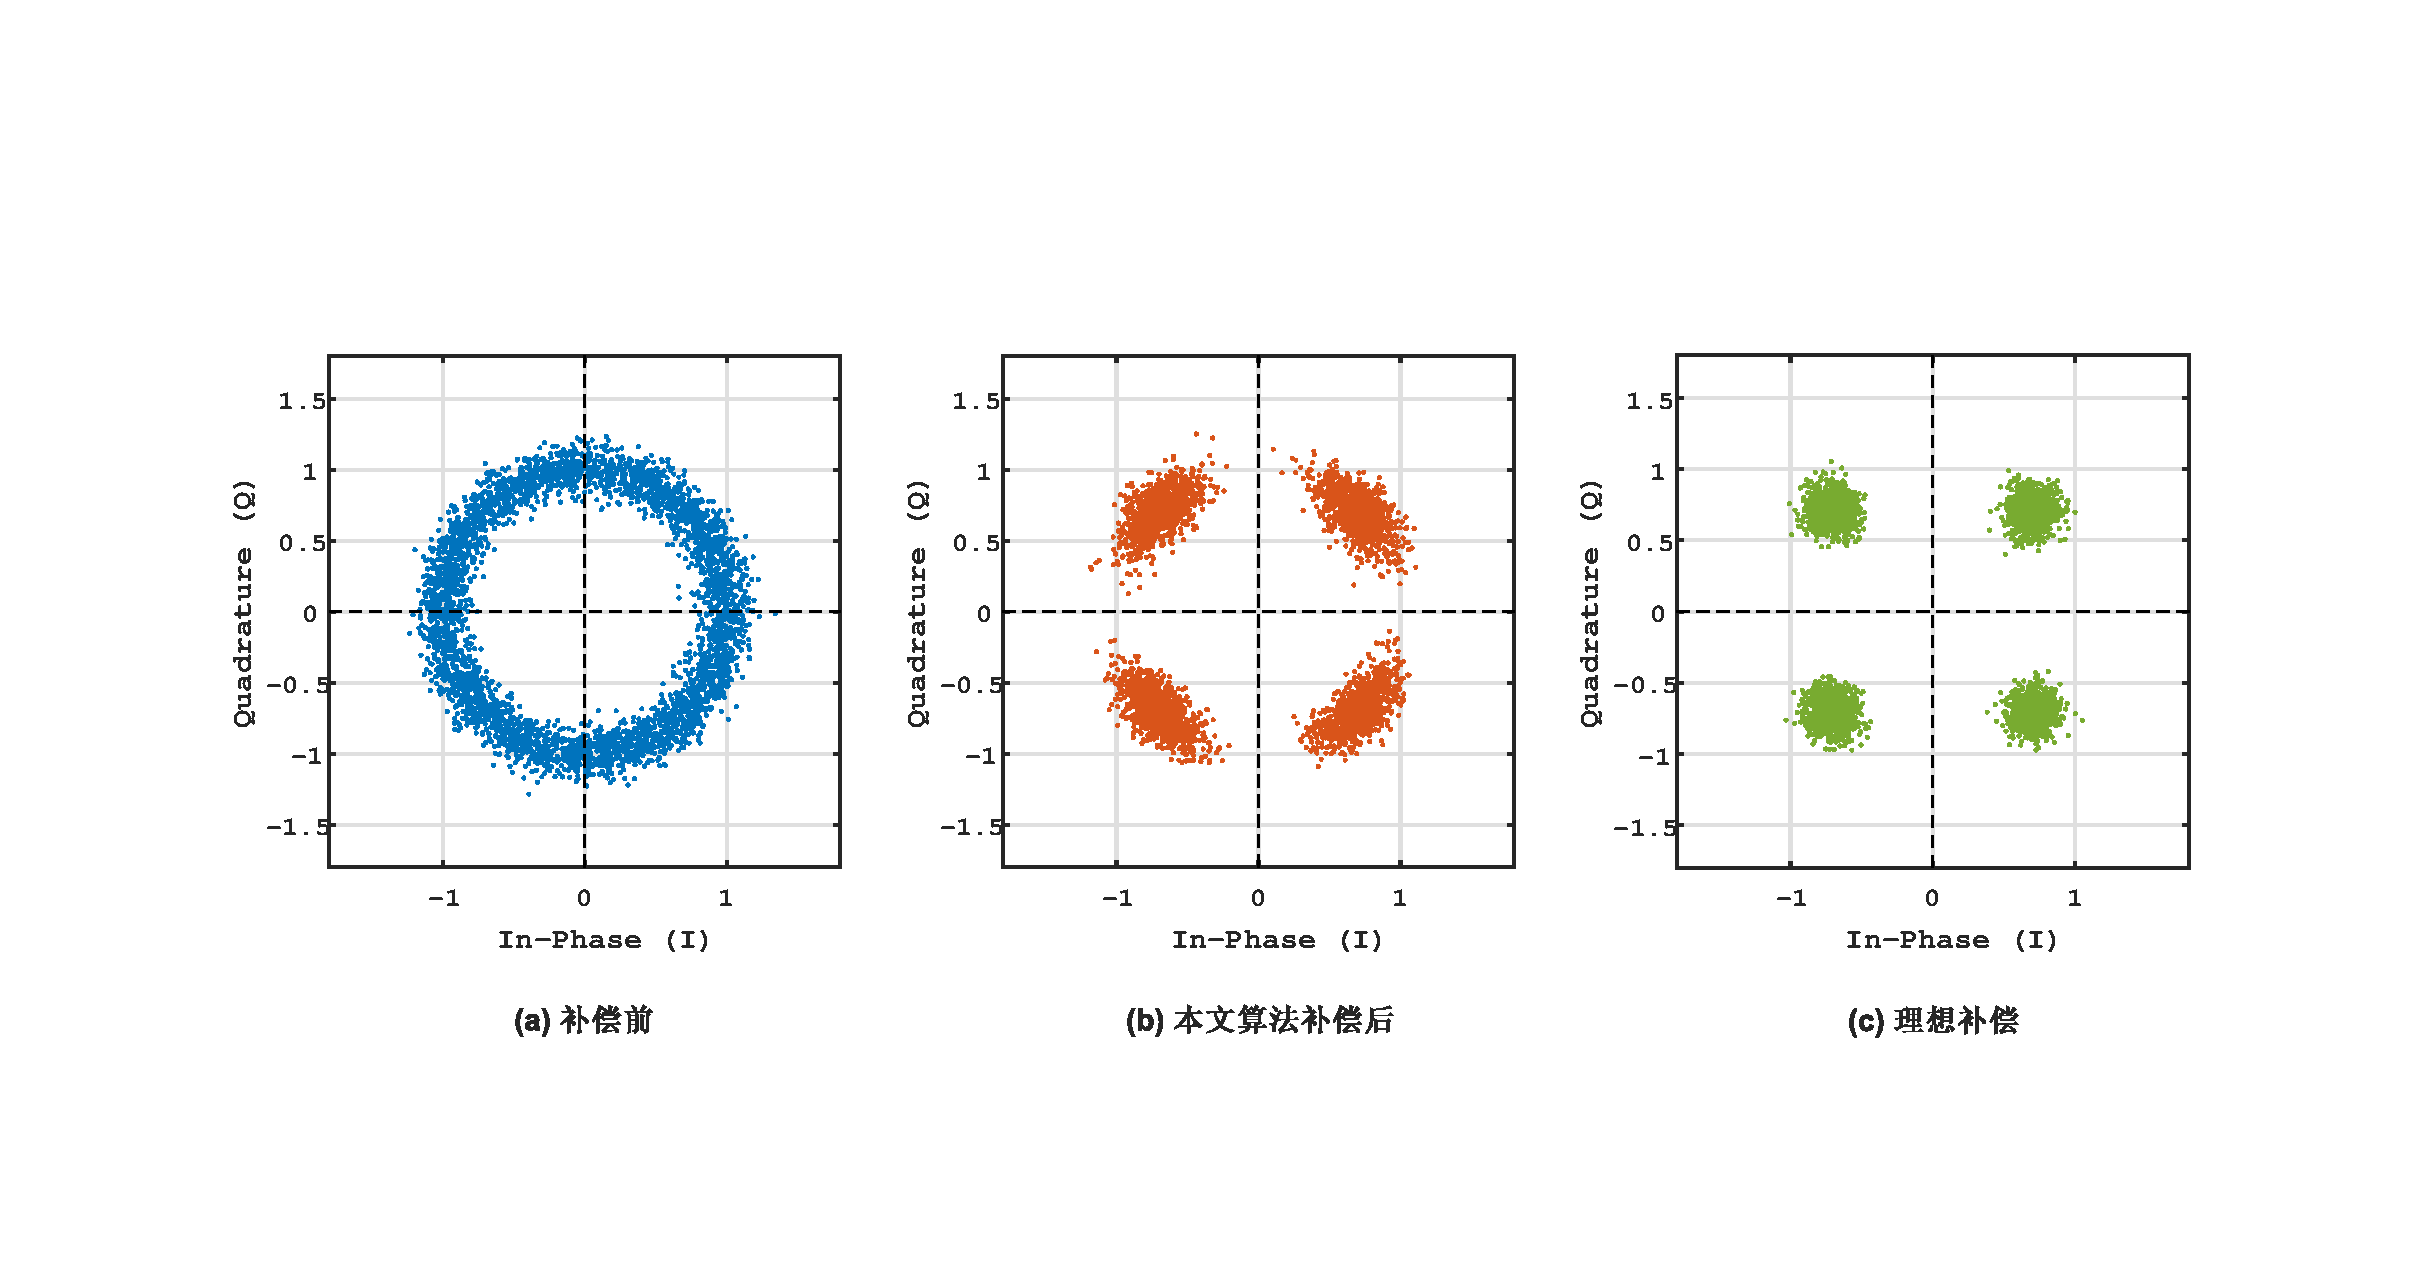
\includegraphics[width=0.85\linewidth]{figures/fig10_HighDynamic_CIR.eps}
    \caption{高动态水下信道冲激响应三维演化图（$N=256$，$P=4$，$f_d=0.15$）} 
    \label{fig:high_dynamic_cir}
\end{figure}

由图~\ref{fig:high_dynamic_cir} 可见，X 轴方向对应多径时延（Tap Index），反映了不同路径之间的到达时间差异；Y 轴方向对应符号时间维度（Sample Index），体现了信道随时间的快速变化特征；Z 轴幅度则反映了各路径在不同时刻的复增益起伏程度。从图中可以清晰观察到，在归一化多普勒频移 $f_d=0.15$ 的高动态条件下，各条路径的复增益沿时间轴呈现出剧烈波动，说明信道在符号周期内已不能近似为准静态，而是具有明显的时变特征。这种时延与多普勒的双重扩展正是本章系统模型所刻画的双选择性信道核心特征，也是所提基于静默位置泄露能量最小化方法需要应对的主要物理挑战。与第三章低动态场景中信道在整个符号周期内近似恒定的情形形成鲜明对比，本章的高动态信道要求接收端不仅具备多径均衡能力，还必须能够感知并补偿由多普勒效应引起的载波频偏，这进一步验证了从 IM-DD 架构转向相干架构的必要性。

为了更加清晰地刻画所提盲补偿策略的有效性，本文进一步设置三种对比方案：其一为理想下界（Ideal），即假设接收端已知准确残余 CFO 且无需任何额外开销，用于表征理论最佳性能；其二为传统显式导频方案（Conventional Pilot-LS），即强制占用 20\% 静默位置作为导频并采用最小二乘准则进行残余 CFO 估计，此时在总发射功率不变的条件下，有效数据维度与对应能量分配将受到惩罚；其三为本文所提零导频开销方案（Proposed），即利用一维频偏网格盲搜索，直接寻找使静默位置残余泄露能量最小的频偏补偿参数。通过这三种方案的并列比较，可以同时评估本文方法在性能逼近能力和频谱效率保持能力上的综合优势。为便于读者在后续 BER、导频开销和线宽鲁棒性结果之间建立对应关系，表~\ref{tab:cfo_strategy_comparison} 对三类残余 CFO 补偿策略的资源占用与性能特性进行了归纳。

\begin{table}[htbp]
    \centering
    \caption{不同残余 CFO 补偿策略的开销与性能特性对比表}
    \label{tab:cfo_strategy_comparison}
    \begin{tabular}{p{2.1cm}p{2.0cm}p{1.8cm}p{2.0cm}p{2.1cm}p{1.8cm}p{1.8cm}}
        \toprule
        补偿策略 & 参考信息来源 & 额外导频开销 & 估计/搜索方式 & 对维纳相位噪声的鲁棒性 & 与理想性能的接近程度 & 适用条件 \\
        \midrule
        Ideal & 已知真实残余 CFO & 无 & 无需估计，作为理论下界 & 最强 & 最优下界 & 用于性能基准，不具工程可实现性 \\
        Conventional Pilot-LS & 显式导频位置 & 有，约 20\% & 最小二乘或导频残差最小化 & 中等 & 受导频开销与估计偏差限制 & 适合可接受资源挤占的传统方案 \\
        Proposed & 静默位置零结构先验 & 无额外导频 & 稀疏度量粗搜索 + 泄露能量最小化交替优化 & 较强 & 接近理想下界 & 适合高动态 UWOC 中频谱效率敏感场景 \\
        \bottomrule
    \end{tabular}
\end{table}

\subsection{高动态场景下的 BER 性能对比}
\label{subsec:high_mobility_ber} 

图~\ref{fig:coherent_ber_high_mobility} 给出了高动态场景下相干 AFDM-IM 与基准 OFDM-IM 的 BER 随 SNR 变化的对比结果。设收发平台之间存在较大相对运动速度，使归一化最大多普勒频移达到高动态条件。

\begin{figure}[htbp]
    \centering
    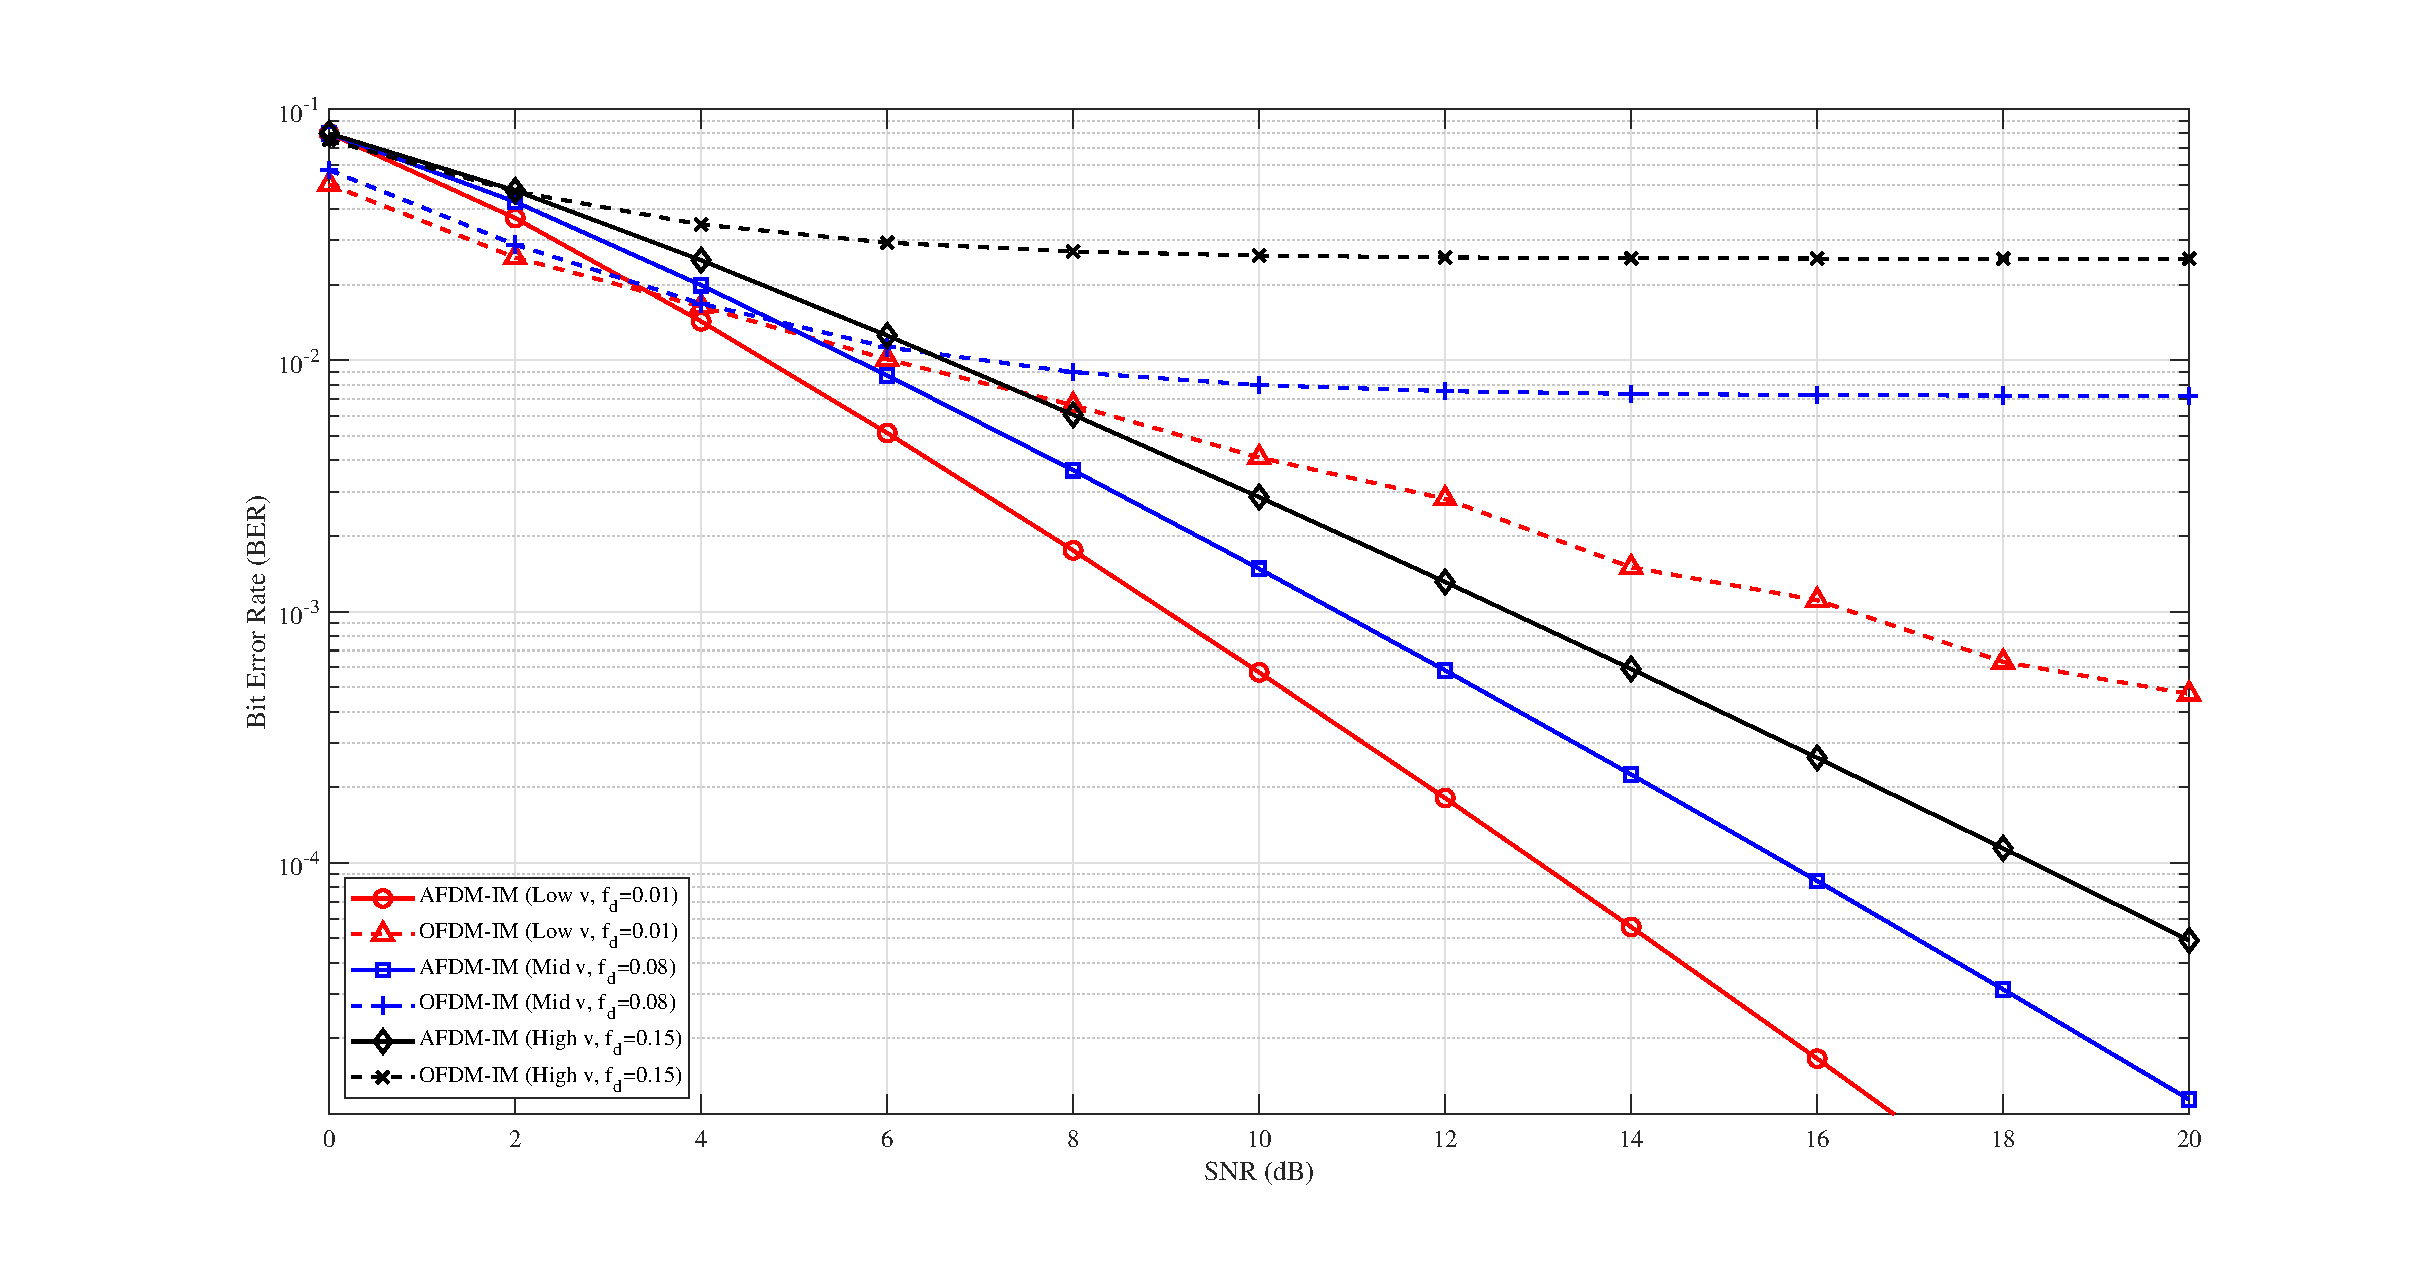
\includegraphics[width=1\linewidth]{figures/fig6_coherent_ber_high_mobility.eps}
    \caption{高动态场景下不同相干索引调制方案的 BER 性能对比}  
    \label{fig:coherent_ber_high_mobility}
\end{figure}

由图~\ref{fig:coherent_ber_high_mobility} 可见，所提相干 AFDM-IM 在整个观测 SNR 区间内均优于相干 OFDM-IM。随着 SNR 提高，OFDM-IM 受多普勒引起的 ICI 影响更加明显，而 AFDM-IM 由于在 DAFT 域中具有更适合双选择性信道处理的结构，因此仍能保持显著的性能增益。

上述结果首先验证了本文所提波形层设计的基础优势，即在进一步讨论残余 CFO 补偿开销之前，AFDM-IM 相对于 OFDM-IM 已经在高动态条件下展现出更强的抗多普勒能力。这一结果为后续进一步研究“在 AFDM-IM 框架内如何低开销地补偿主导残余频偏并对维纳相位噪声保持鲁棒性”提供了必要前提：只有当波形本身能够有效抑制高动态场景中的时延--多普勒扩散时，静默位置泄露能量最小化这一接收策略才具有进一步逼近理想性能的现实意义。

上述结果表明，高动态条件下系统性能瓶颈并不完全来自噪声本身，而更多来自波形对双选择性信道的适应能力差异。当 SNR 较低时，噪声仍是影响 BER 的主要因素，两种方案之间的性能差距相对有限；随着 SNR 提升，噪声影响逐渐减弱，波形结构对多普勒扩展的适应能力开始主导系统性能，此时 OFDM-IM 中由频域正交性破坏引起的 ICI 更加突出，而 AFDM-IM 则因其在 DAFT 域中的结构优势表现出更稳定的误码率下降趋势。

从机理上看，AFDM 波形能够将高动态信道中的时延与多普勒扩展映射为更具规律性的等效耦合结构，因此接收端在进行最大似然判决时可更有效地区分有用信号与干扰项。相比之下，OFDM-IM 在频偏和时变影响下更容易出现跨子载波能量扩散，导致激活位置判决和活动符号判决同时恶化。这也说明，在高动态 UWOC 中，单纯依赖 OFDM 结构叠加索引调制机制难以从根本上克服多普勒引起的性能退化，而 AFDM 与索引调制的结合更适合此类场景。

\subsubsection{AFDM 与 OFDM 在高动态场景下的性能差异机理}

为更深入理解 AFDM-IM 相较 OFDM-IM 的性能优势来源，本节从变换域能量分布与等效信道结构两个角度进行分析。在高动态场景下，多普勒频移会破坏传统 OFDM 的子载波正交性，导致严重的载波间干扰。具体而言，当归一化多普勒频移为 $f_d$ 时，OFDM 接收端第 $k$ 个子载波上的观测信号可近似表示为
\begin{equation}
Y_{\mathrm{OFDM}}[k] = H[k]X[k] + \sum_{m \neq k} H[m]X[m] \cdot \mathrm{sinc}(\pi(f_d N + k - m)) + W[k]
\end{equation}
其中，第一项为期望信号分量，第二项为来自其他子载波的 ICI 分量，$\mathrm{sinc}(\cdot)$ 函数的旁瓣衰减速度决定了 ICI 的扩散范围。当 $f_d$ 较大时，$\mathrm{sinc}$ 函数主瓣展宽，旁瓣能量增强，导致相邻子载波之间的能量泄露显著增加。

相比之下，AFDM 通过引入啁啾参数 $c_1$ 和 $c_2$，使信号在 DAFT 域中获得对时延--多普勒耦合更具适应性的表示形式。在 DAFT 域中，多普勒频移引起的时域线性相位斜坡会被映射为特定的位置偏移，而非像 OFDM 那样表现为全局性的子载波间能量扩散。具体而言，当存在归一化多普勒频移 $f_d$ 时，AFDM 接收端 DAFT 域第 $k$ 个位置的等效响应可近似表示为
\begin{equation}
Y_{\mathrm{AFDM}}[k] \approx \sum_{p=1}^{P} h_p e^{j\phi_p} X[(k - \Delta k_p)_N] + W[k]
\end{equation}
其中，$\Delta k_p = 2Nc_1(l_p + f_d \cdot n_p)$ 为第 $p$ 条路径在 DAFT 域中的等效位置偏移，$\phi_p$ 为对应的相位旋转。该式表明，多普勒效应在 AFDM 中主要表现为 DAFT 域位置的确定性偏移，而非随机性的全局能量扩散。当啁啾参数设计合理时，不同路径对应的偏移位置可保持分离，接收端能够通过结构化检测算法联合利用多条路径的能量，从而获得多径分集增益。

上述分析揭示了 AFDM-IM 相较 OFDM-IM 在高动态场景下性能优势的本质：OFDM 将多普勒效应视为破坏正交性的有害因素，其 ICI 随多普勒强度增大而迅速恶化；而 AFDM 通过啁啾映射将多普勒扩展转化为 DAFT 域中的结构化位置偏移，使接收端能够在变换域中更有效地分离和利用多径分量。这种结构化表示能力正是图~\ref{fig:coherent_ber_high_mobility} 中 AFDM-IM 曲线在高 SNR 区间仍保持稳定下降、而 OFDM-IM 曲线出现明显平台的根本原因。

\subsection{不同残余 CFO 补偿策略下的 BER 性能对比} 
\label{subsec:blind_phase_ber}

在验证 AFDM-IM 波形本身的高动态鲁棒性之后，进一步需要考察：当系统同时受到残余频偏与维纳相位噪声影响时，所提基于静默位置泄露能量最小化的盲补偿策略，能否在不额外占用导频资源的条件下保持接近理想残余 CFO 补偿的性能。图~\ref{fig:blind_phase_ber_compare} 给出了不同残余 CFO 补偿策略下相干 AFDM-IM 系统的 BER 对比结果。

\begin{figure}[htbp] 
    \centering
    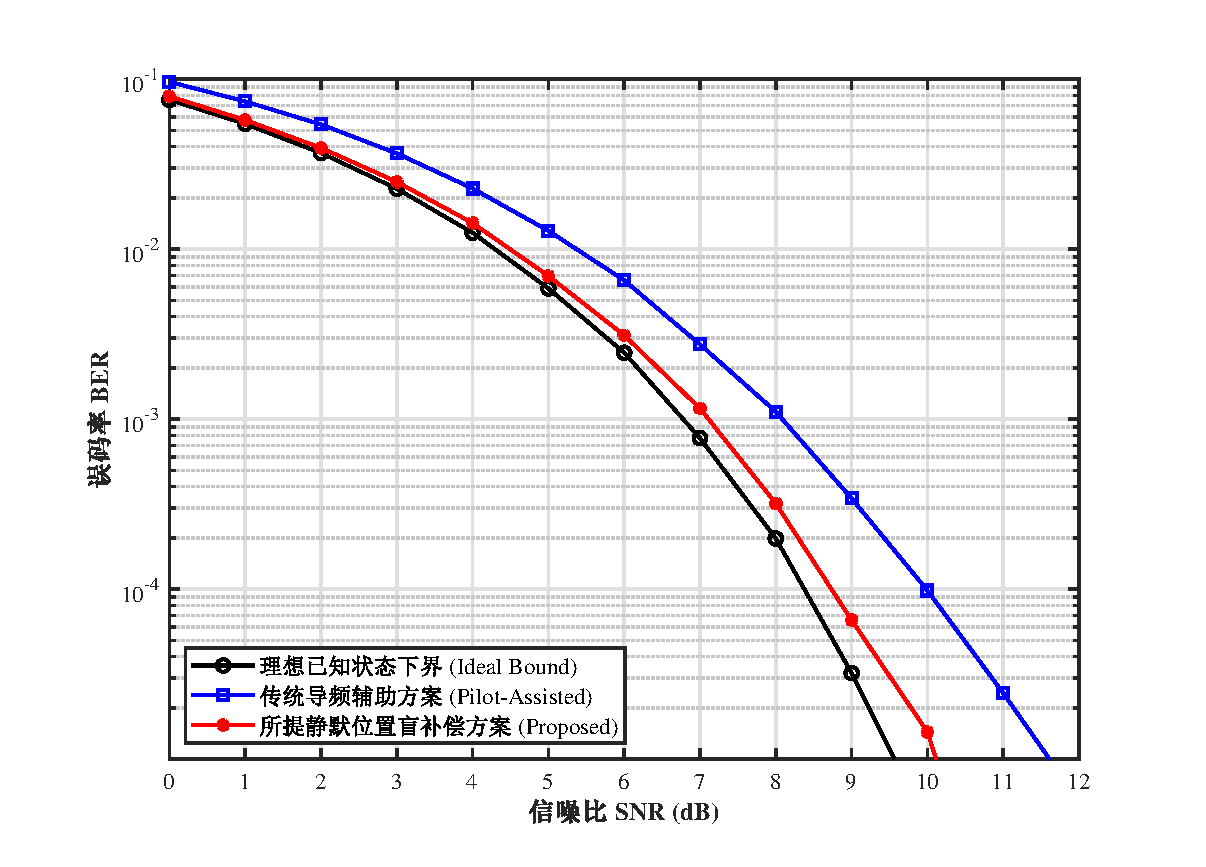
\includegraphics[width=1\linewidth]{figures/fig8_BER_COMPARE.eps} 
    \caption{不同残余 CFO 补偿策略下相干 AFDM-IM 系统的 BER 性能对比}
    \label{fig:blind_phase_ber_compare}
\end{figure}

图~\ref{fig:blind_phase_ber_compare} 中，Ideal 曲线对应理想残余 CFO 已知下界，即假设接收端准确获知主导频偏参数且无需任何训练开销；Conventional Pilot-LS 曲线对应传统显式导频方案，即强制占用 20\% 的静默位置作为导频并进行最小二乘残余 CFO 估计；Proposed 曲线则对应本文方法，即在 0 导频开销条件下，通过一维频偏网格盲搜索直接最小化静默位置残余泄露能量。三种方案的对比能够同时反映主导频偏估计精度与资源开销之间的关系。

由图可见，传统 Pilot-LS 曲线相较于理想下界整体出现明显劣化，并呈现出向右上方偏移的趋势。在相同总发射功率约束下，这种退化并不完全来自估计误差本身，更重要的原因在于：当 20\% 的静默位置被强制改作显式导频后，原本可用于维持索引结构与数据传输的有效物理资源被部分占用，从而对数据分量引入了额外的信噪比惩罚。仿真结果表明，在典型 BER 工作区间内，该导频开销对应的性能损失约为 1 dB，这说明传统显式导频方法虽然能够完成主导频偏跟踪，但其代价是以牺牲频谱效率和有效能量利用率为前提的。

为更清晰地理解上述 1 dB 性能损失的来源与含义，下面从资源分配角度给出定量分析。此处所称典型 BER 工作区间定义为 $10^{-3}$ 至 $10^{-5}$ 量级，对应前向纠错译码前系统实现高可靠通信所需的误码率范围。在该区间内，BER 曲线处于下降段，SNR 的微小变化将直接映射为 BER 的显著改变，因此资源开销引起的等效 SNR 惩罚在此区间内对系统性能的影响最为敏感。当传统方案强制将 20\% 的静默位置改为显式导频时，在总发射功率不变的条件下，有效数据子载波所分得的能量占比降为原来的 80\%。由此导致的等效 SNR 惩罚可精确计算为
\begin{equation}
    \Delta_{\mathrm{SNR}} = 10\log_{10}\!\left(\frac{1}{1-\eta_p}\right) = 10\log_{10}\!\left(\frac{1}{0.8}\right) \approx 0.97\,\mathrm{dB}
    \label{eq:snr_penalty}
\end{equation}
其中，$\eta_p=0.2$ 为导频占用比例。图~\ref{fig:alloc_snr_penalty} 以柱状折线组合图的形式直观展示了这一资源分配差异与对应的 SNR 惩罚。

\begin{figure}[htbp]
    \centering
    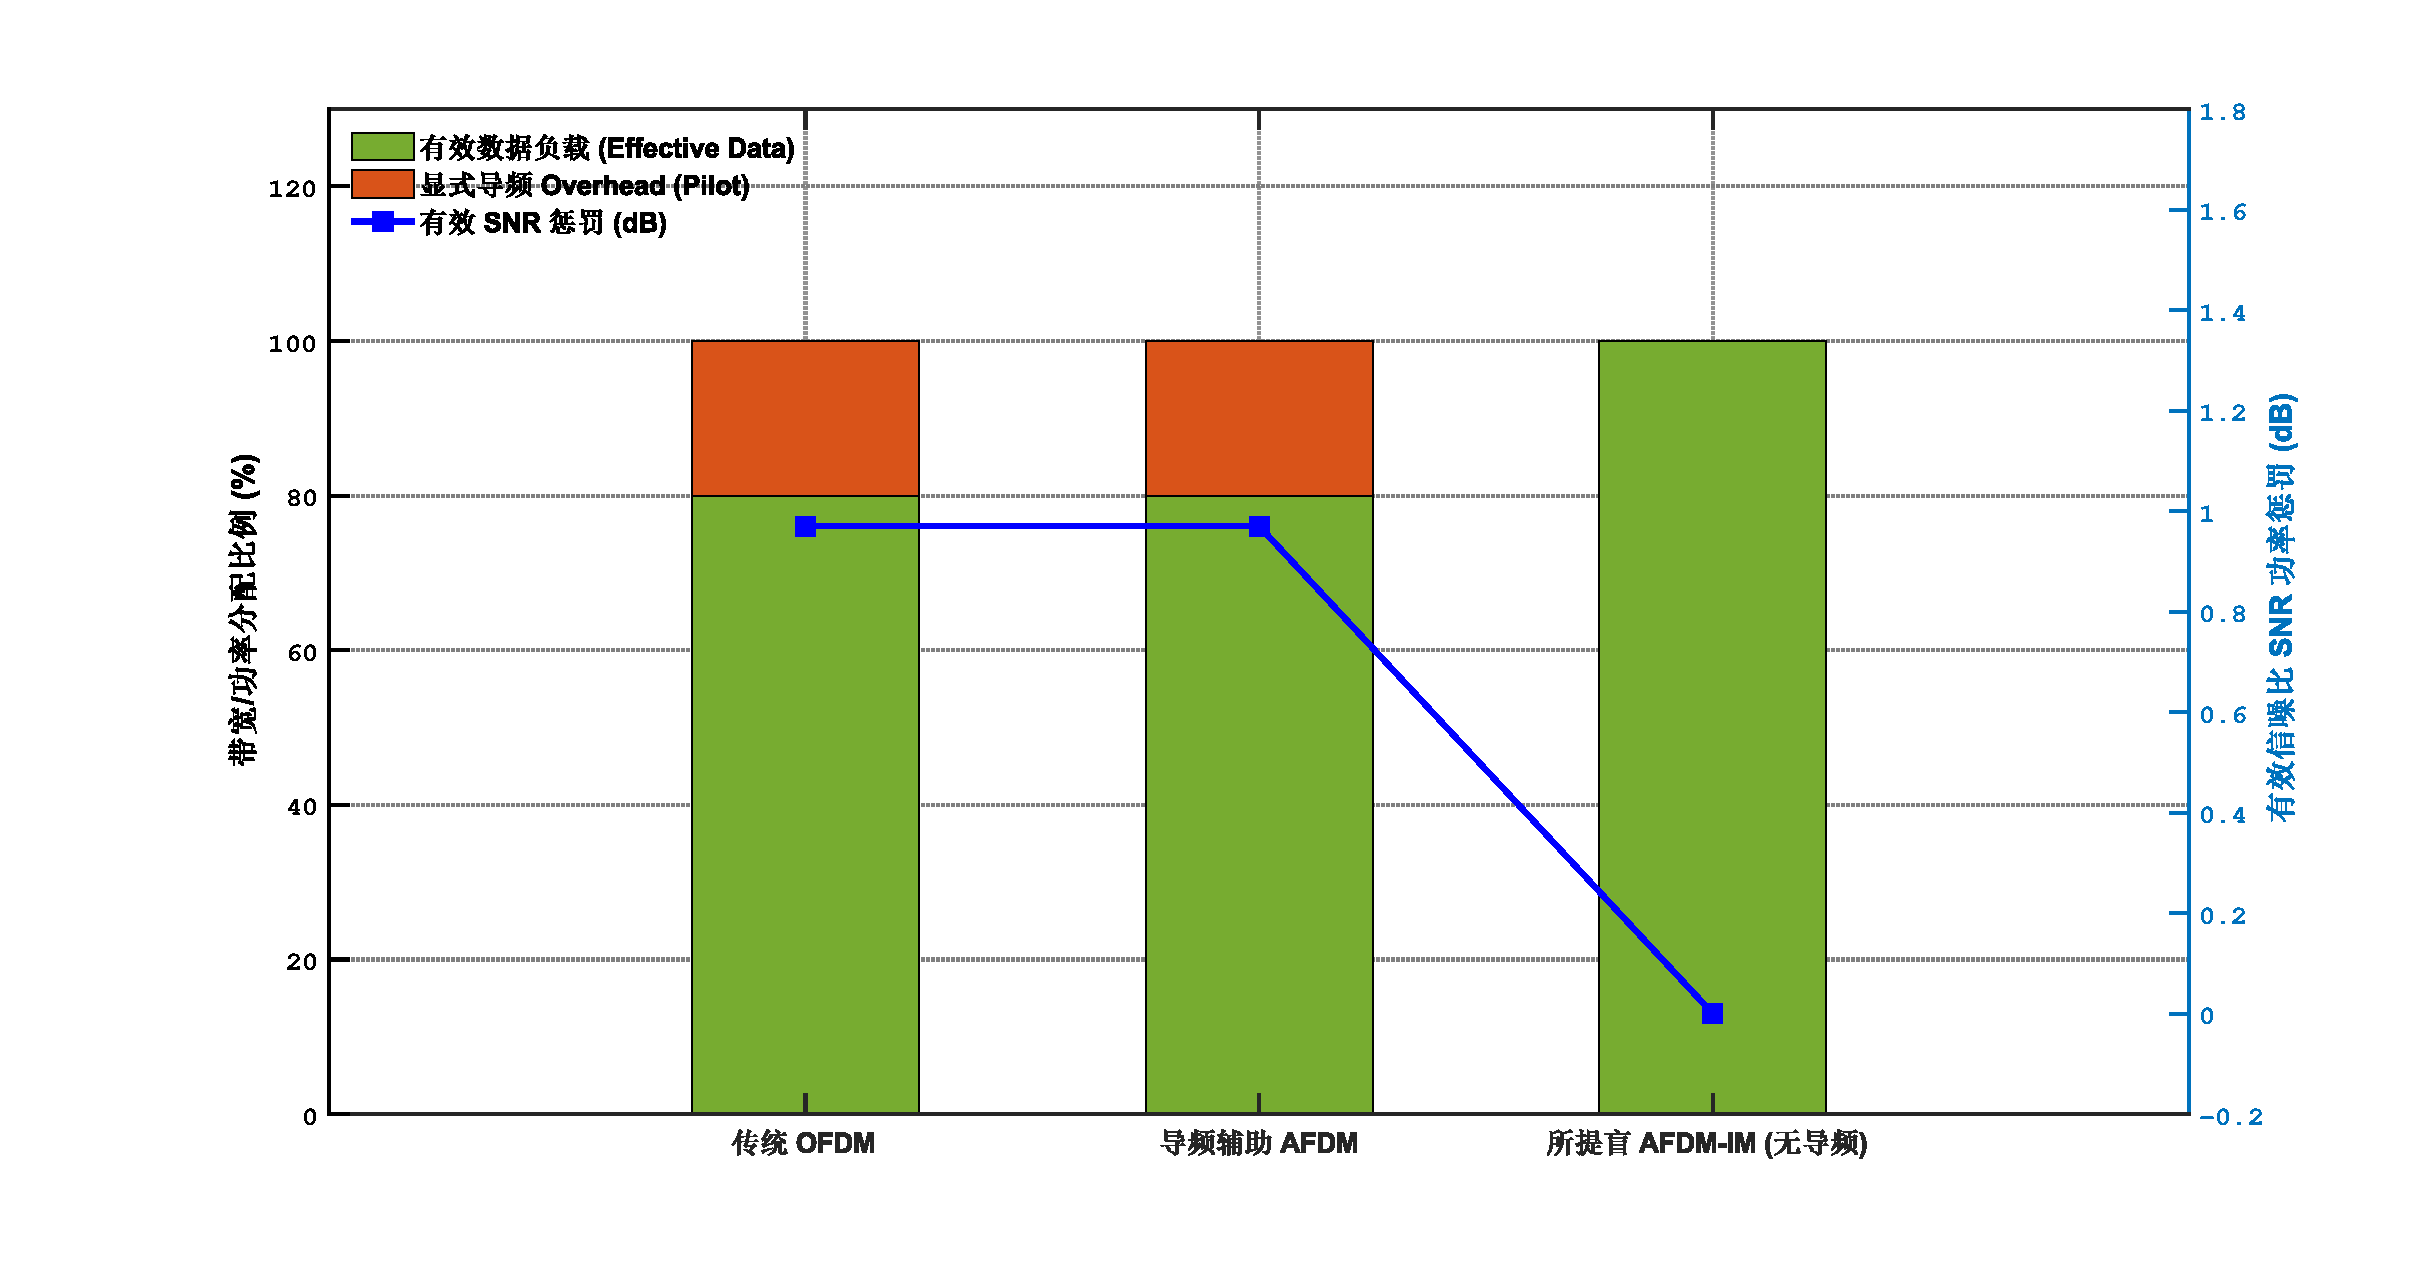
\includegraphics[width=0.85\linewidth]{figures/fig11_Alloc_SNR_Penalty.eps}
    \caption{不同方案的资源分配对比与导频开销引起的等效 SNR 惩罚} 
    \label{fig:alloc_snr_penalty}
\end{figure}

由图~\ref{fig:alloc_snr_penalty} 左轴堆叠柱状图可见，传统 Pilot-LS 方案中有 20\% 的物理资源被强制分配为显式导频，有效数据占比仅为 80\%；而本文所提方案中，由于完全利用 AFDM-IM 天然静默位置作为隐式参考，无需额外预留导频，因此 100\% 的发送资源均可用于有效数据传输。右轴蓝色折线则定量展示了这 20\% 资源浪费所对应的约 0.97 dB 等效 SNR 惩罚。这一损失虽在数值上看似有限，但在典型 BER 工作区间（$10^{-3}\sim10^{-5}$）内，由于 BER 曲线处于瀑布下降区域，约 1 dB 的 SNR 差异可对应数倍甚至一个量级的 BER 变化，从而对系统的可靠传输能力产生实质性影响。因此，本文方法通过避免任何显式导频开销，不仅在频谱效率上具有明确优势，更在有效信噪比层面为数据检测保留了约 1 dB 的额外余量。

相比之下，本文所提 Proposed 曲线与 Ideal 曲线在整个观测 SNR 区间内几乎保持重合，表明所提盲补偿策略能够在不预留任何额外导频的条件下，实现接近理想残余 CFO 已知情形的检测性能。其根本原因在于，AFDM-IM 中天然存在的大量静默位置为接收端提供了可靠的隐式零参考；当频偏补偿参数取值正确时，泄露到静默位置上的残余能量将被显著压缩，因此通过一维频偏网格搜索最小化这部分能量，能够以较高精度恢复主导残余频偏。换言之，本文方法并非直接估计纯常数相位或完整维纳相位噪声过程，而是将传统基于显式非零导频的残差最小化转换为基于隐式零参考的泄露能量最小化，从而在保持高估计精度的同时避免了额外训练开销。

这一结果在数学与工程两个层面都具有重要意义。从数学角度看，Proposed 曲线逼近 Ideal 下界，说明静默位置零结构确实能够作为有效约束参与残余 CFO 参数估计，验证了本文前述建模与交替优化思想的合理性；从工程角度看，该结果进一步证明，在带宽和发射资源极其宝贵的高动态 UWOC 场景中，利用接收端搜索迭代所带来的额外计算量，去换取近乎无损的频谱效率，是一种极具吸引力的实现路径。特别是在相干链路已具备数字信号处理平台的条件下，这种“以算力换频谱”的设计权衡相比传统显式导频方案更具实际优越性。

\subsection{激光器线宽对系统性能的影响}
\label{subsec:phase_noise_sim}

除多普勒频移外，相干 UWOC 系统还会受到激光器有限线宽引起的相位噪声影响。图~\ref{fig:coherent_phase_noise} 给出了不同组合线宽条件下所提相干 AFDM-IM 系统的 BER 结果。前一小节侧重比较不同残余 CFO 补偿策略在固定典型扰动条件下的有效性，而本小节则进一步从器件非理想程度变化的角度，考察系统对不同强度维纳相位噪声的整体鲁棒性，因此两组结果具有互补关系。

\begin{figure}[htbp]
    \centering
    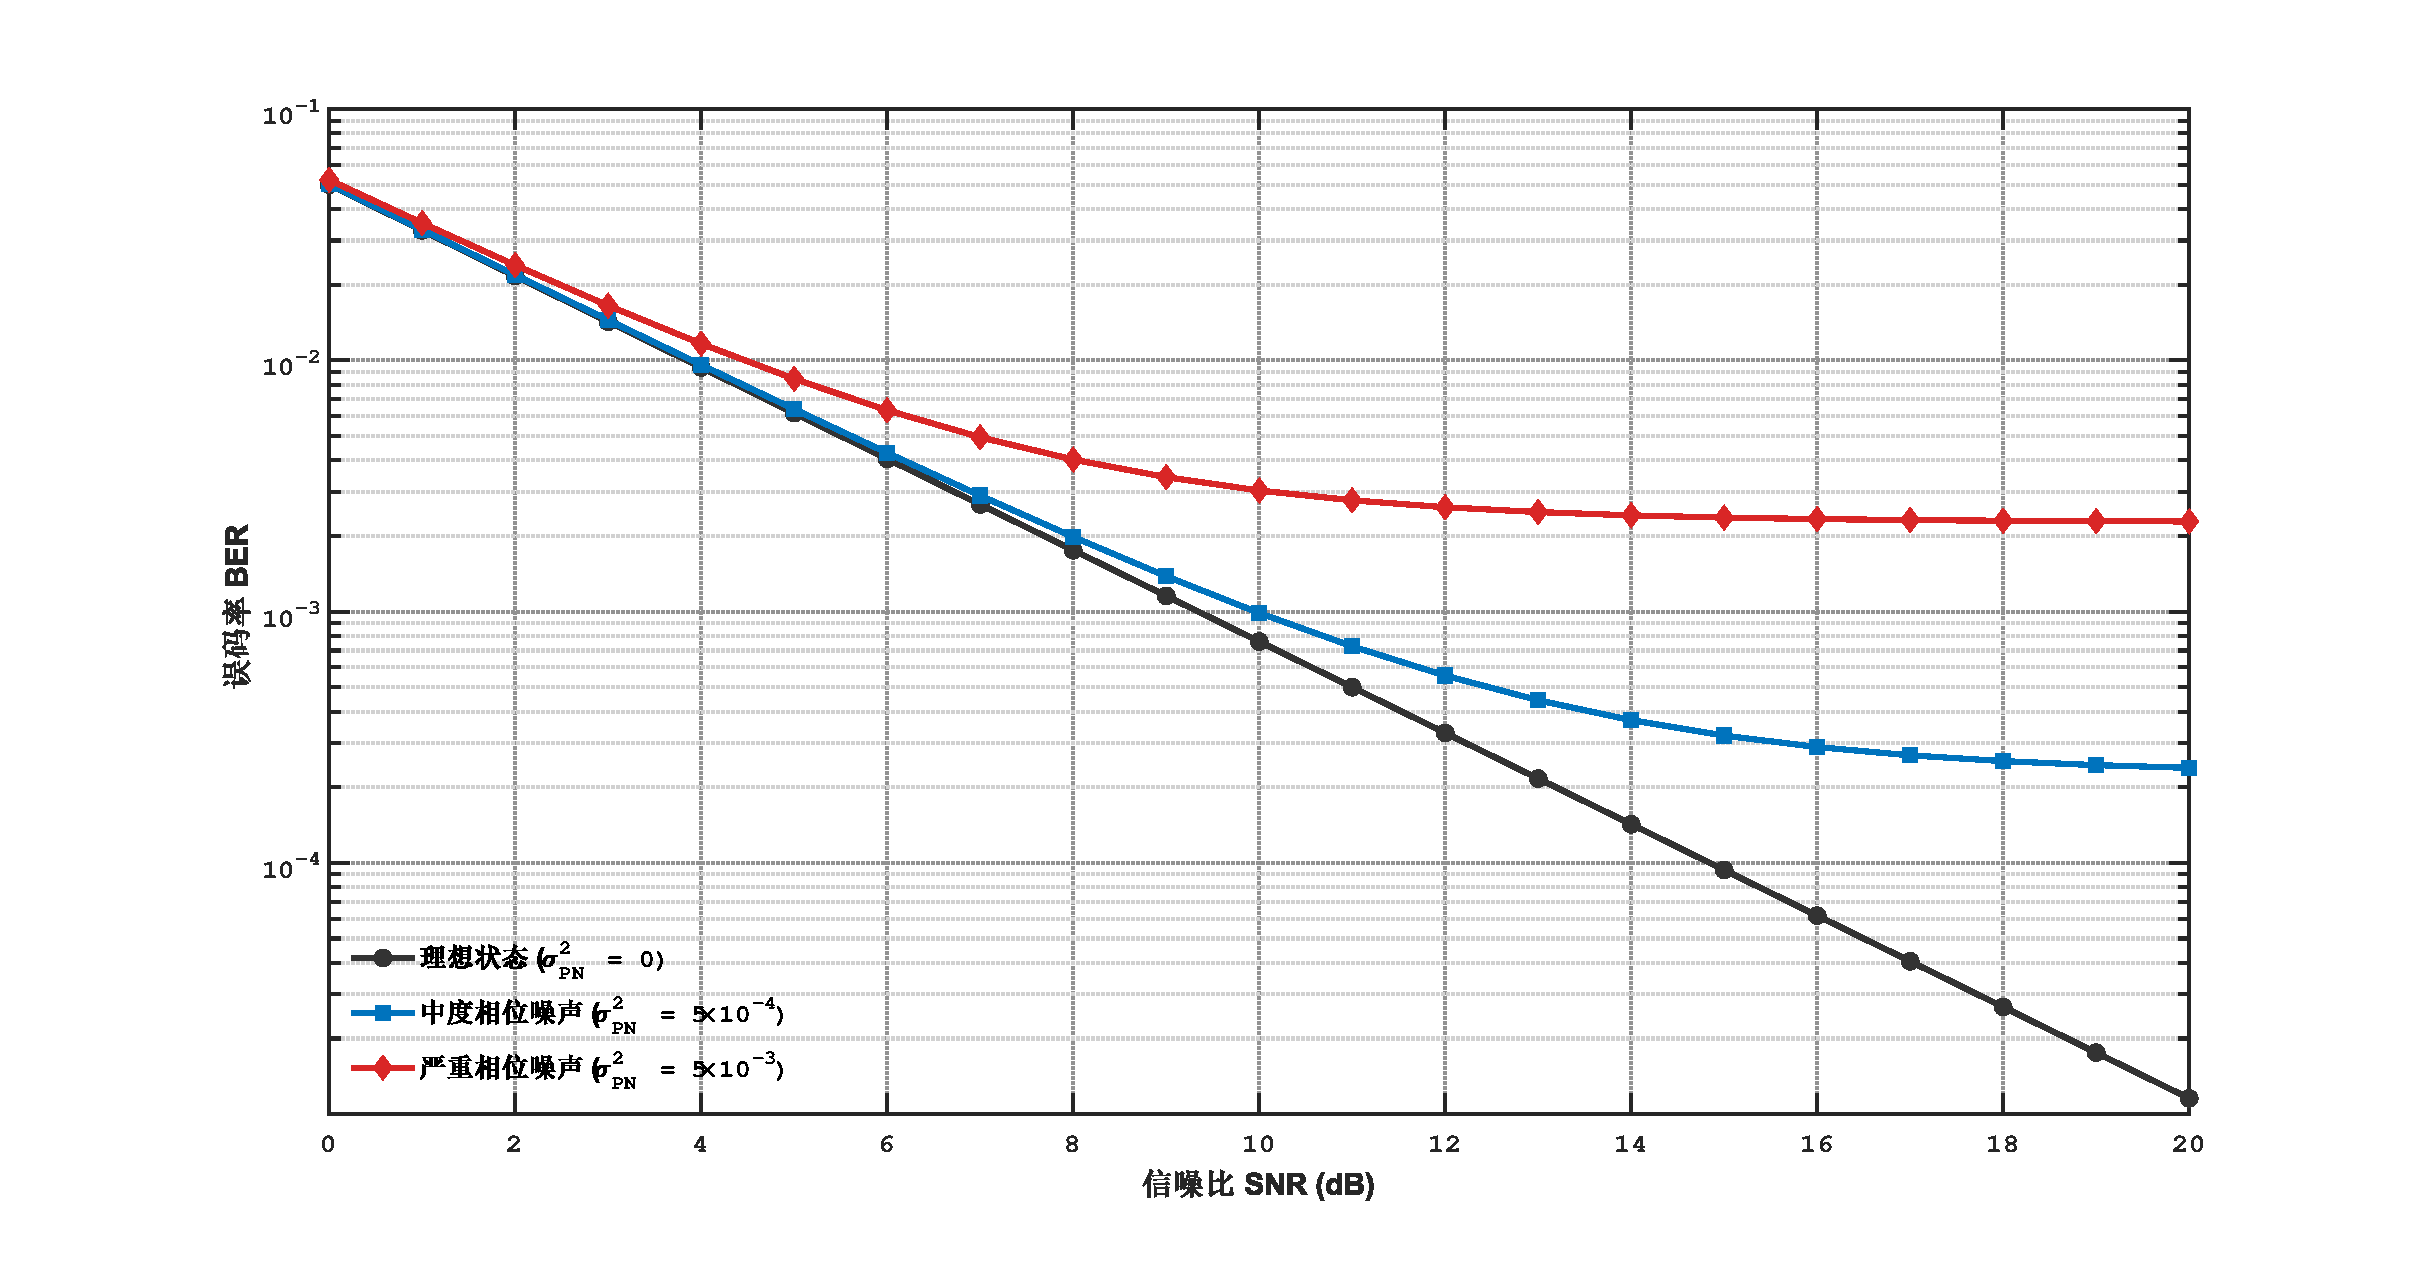
\includegraphics[width=0.85\linewidth]{figures/fig7_coherent_phase_noise.eps}
    \caption{不同激光器线宽条件下相干 AFDM-IM 系统的 BER 性能}
    \label{fig:coherent_phase_noise}
\end{figure}

由图~\ref{fig:coherent_phase_noise} 可见，随着组合线宽增大，系统 BER 曲线整体向高 SNR 方向移动，说明相位噪声会削弱系统性能。结合第~\ref{subsec:silent_leakage_principle} 节的分析，该现象具有明确的物理解释：本文所提算法的核心目标是补偿多普勒效应引起的主导载波频偏，而维纳相位噪声作为逐点时变的随机游走过程，无法被单一频偏参数 $\theta$ 所消除，其效应在算法框架中被归入等效残余干扰。当组合线宽 $\Delta\nu$ 增大时，单符号内维纳相位噪声的累积方差 $2\pi\Delta\nu T_{\mathrm{sym}}$ 随之上升，残余随机扰动对 DAFT 域正交性的破坏程度增强，从而导致即使在频偏已被正确补偿的前提下，系统仍面临更强的等效干扰，BER 相应恶化。但在中等线宽条件下，维纳累积扰动仍处于可控水平，所提方案因此保持了充分的鲁棒性。

进一步分析可知，相位噪声对系统性能的影响主要体现在两个层面。一方面，维纳相位噪声中包含的缓变趋势分量（近似线性漂移部分）可被频偏补偿算法有效吸收，因此不会引起灾难性退化；另一方面，维纳过程中的高阶随机波动分量则会在 DAFT 域引起不可预测的能量扩散，产生无法被确定性参数完全捕获的残余干扰，从而降低基于估计信道进行检测的准确性。当组合线宽较小时，随机波动分量功率有限，系统仍可依靠 AFDM 波形结构和最大似然检测方法保持稳定的判决性能；而当线宽持续增大时，残余随机扰动将逐步成为限制系统 BER 的关键因素。这也从仿真角度验证了第~\ref{subsec:silent_leakage_principle} 节中关于维纳相位噪声作为等效背景干扰这一建模选择的合理性。

该结果进一步验证了，所提方案通过获取高有效信噪比余量，能够对维纳相位噪声引起的残余扰动实现有效的鲁棒容忍。这意味着 AFDM-IM 方案对于高动态相干 UWOC 并非仅在理想激光器条件下有效，而是在实际器件线宽范围内均具备稳定的传输性能。从工程角度看，该结论明确了所提方案在实际系统中的可行性与适用性。

\subsection{不同多普勒强度下的系统鲁棒性全景分析}
\label{subsec:doppler_heatmap}

前述仿真均在固定的归一化多普勒频移条件下进行分析，未全面揭示系统性能随多普勒强度连续变化时的整体趋势。为更完整地评估所提方案与传统 OFDM 方案在不同动态条件下的适应能力差异，本小节通过二维误码率热力图的形式，考察 BER 在 SNR 与归一化多普勒频移构成的联合参数空间中的分布特征。图~\ref{fig:ber_doppler_heatmap} 给出了传统相干 OFDM-IM 方案与本文所提相干 AFDM-IM 方案在相同条件下的对比结果。

\begin{figure}[htbp]
    \centering
    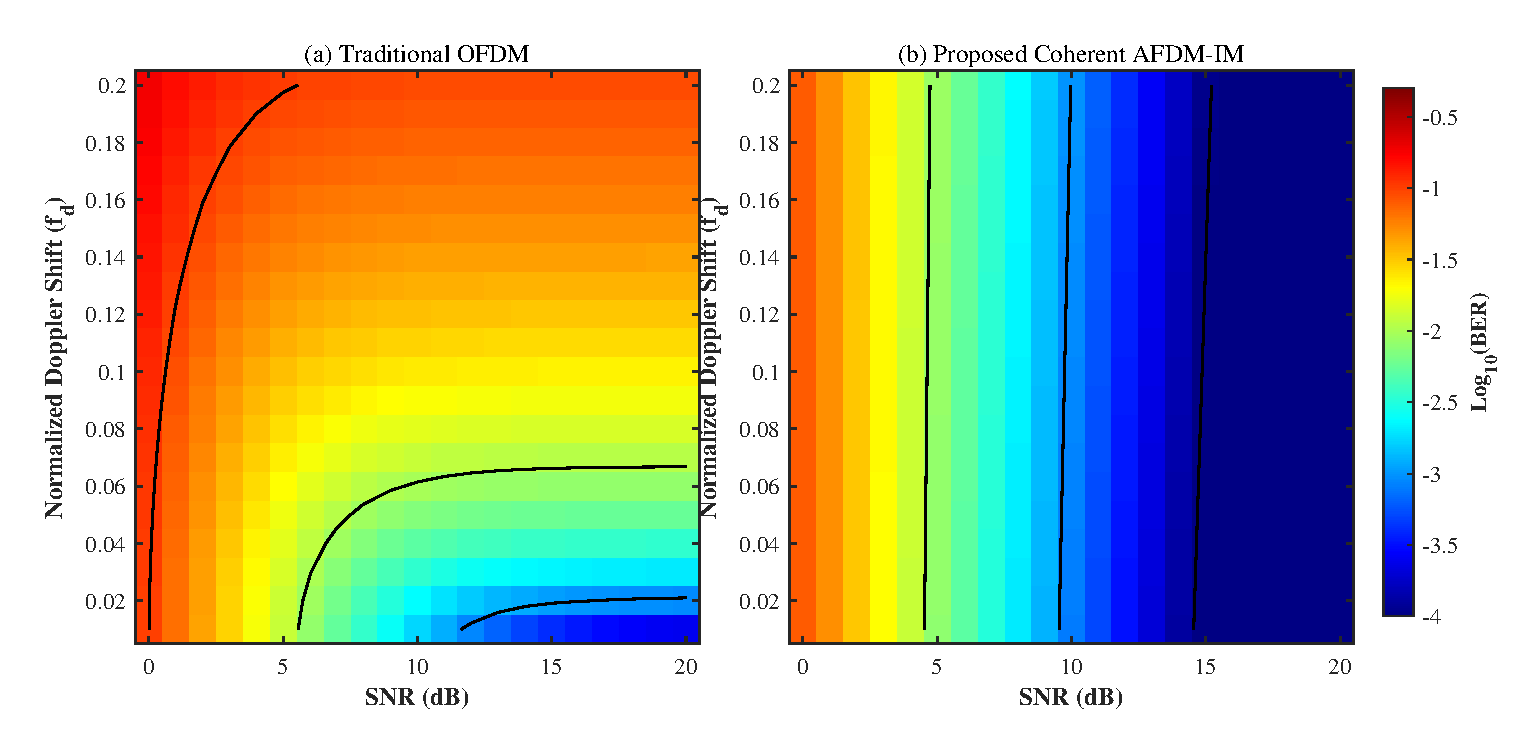
\includegraphics[width=1.0\linewidth]{figures/fig12_BER_Doppler_Heatmap.eps}
    \caption{不同归一化多普勒频移与 SNR 条件下的 BER 二维热力图对比}
    \label{fig:ber_doppler_heatmap}
\end{figure}

由图~\ref{fig:ber_doppler_heatmap}(a) 可以看到，传统 OFDM-IM 方案的 BER 热力图在归一化多普勒频移超过约 0.05 后，高误码区域（红色与黄色区域）迅速向低 SNR 和高 SNR 方向同时扩展，表现为图上部大面积的高 BER 覆盖。这说明传统 OFDM 在多普勒较强时，子载波正交性遭到严重破坏，载波间干扰成为性能主导因素，即使在较高 SNR 条件下也无法通过增大发射功率来有效改善误码率，系统陷入所谓的 ICI 地板效应。尤其当归一化多普勒达到 0.10 以上时，几乎整个 SNR 区间均表现为不可靠传输状态，系统已完全失去实用价值。

相比之下，图~\ref{fig:ber_doppler_heatmap}(b) 中本文所提 AFDM-IM 方案展现出截然不同的特征。在相同的多普勒频移与 SNR 参数空间中，可靠通信区域（深蓝色区域）占据了显著更大的范围。即使在归一化多普勒频移达到 0.15$\sim$0.20 的极端高动态条件下，系统在中高 SNR 区间仍能维持较低的 BER 水平，对应的深蓝色区域持续延伸至热力图的上部。这说明 AFDM 波形通过啁啾参数对时延与多普勒扩展的结构化映射，有效抑制了多普勒增大时的能量扩散效应，使系统在宽泛的动态范围内都能保持可靠传输能力。


从工程应用角度看，上述对比结果具有明确的指导意义。在实际高动态 UWOC 场景中，收发平台之间的相对速度往往不是恒定值，而是随任务状态和机动条件持续变化的。若系统仅在某一固定多普勒条件下表现良好，而在多普勒波动时迅速崩溃，则其工程适用性将受到严重限制。图~\ref{fig:ber_doppler_heatmap} 的二维全景对比表明，所提 AFDM-IM 方案在归一化多普勒频移从 0 到 0.20 的宽泛范围内均保持了比传统方案显著更强的鲁棒性，这意味着该方案能够更好地适应实际水下高动态链路中多普勒频移的不确定性和波动性。
\section{本章小结}

本章围绕高动态 UWOC 场景下的多普勒扩展、残余频偏以及维纳相位噪声等关键失真因素，提出了相干 AFDM-IM 传输方案，并完成了从系统建模、接收方法设计到误码性能验证的完整分析。在相干接收架构下引入 AFDM 波形与索引调制机制，建立了包含多径、多普勒频移和维纳相位噪声的统一时域与 DAFT 域系统模型，说明了高动态场景中的检测问题本质上是一个围绕双选择性信道与器件非理想共同展开的联合恢复问题。

本章的研究表明，相干 AFDM-IM 并不是 AFDM 与 IM 的简单叠加，而是一种围绕高动态 UWOC 主导失真机理所构建的系统化方案：AFDM 提供双选择性信道下的波形适配能力，索引调制提供可利用的结构先验，相干接收提供复数域高灵敏度处理基础，而基于静默位置的残余 CFO 感知与检测机制则进一步把发送结构资源转化为接收端低开销自感知能力。上述设计共同构成了面向高动态水下光通信的完整技术链路。

\chapter{总结与展望}
\label{chap:conclusion}

\section{全文总结}
\label{sec:conclusion_summary}

本文围绕复杂水下环境中的AFDM无线光通信关键技术展开研究，针对低动态多径场景与高动态双选择性场景分别提出了两类传输方案，并从系统建模、参数设计、检测方法和误码性能等方面进行了分析与验证。

针对低动态水下场景中散射主导的频率选择性衰落问题，本文提出了ACO-AFDM传输方案。该方案将ACO机制与AFDM调制相结合，在满足IM-DD架构非负实值约束的前提下，利用DAFT域啁啾结构增强系统对多径传播的适应能力。通过数学推导证明了限幅噪声仅分布于偶数子载波位置，保证了ACO机制在AFDM框架下的有效性；推导了啁啾参数 $c_1$ 的设计准则，建立了奇异点规避与多径分离条件；从等效信道矩阵结构角度揭示了ACO-AFDM非对角信道相较于 ACO-OFDM 对角信道的本质优势。仿真结果表明，ACO-AFDM 在双径信道下相较 ACO-OFDM 可获得约 2 dB 的性能增益，且在路径数从 2 增至 10 的鲁棒性测试中性能退化速度显著慢于传统光 OFDM 方案。

针对高动态水下场景中多普勒扩展与相位噪声的联合失真问题，本文提出了相干AFDM-IM传输方案。该方案在相干接收架构下引入AFDM波形与索引调制机制，建立了包含多径、多普勒频移和维纳相位噪声的统一系统模型。利用AFDM-IM静默位置的零结构先验，提出了基于泄露能量最小化的盲残余 CFO 补偿方法，在无额外导频开销下实现主导频偏的精准补偿，并对维纳相位噪声保持鲁棒容忍。通过代价函数全局收敛性分析证明了盲搜准则的可靠性，并定量推导了传统 20\% 导频开销所引起的约 0.97 dB 等效 SNR 惩罚。仿真结果表明，所提方案在高动态条件下显著优于基准 OFDM-IM，在归一化多普勒频移 0 至 0.20 的宽泛范围内均保持可靠通信能力。表~\ref{tab:thesis_contribution_summary} 对全文两类核心场景、对应架构选择、关键方法与主要性能结论进行了集中归纳，可作为本文技术主线的最终摘要。

在系统设计方面，本文建立了包含多径传播、多普勒频移以及维纳相位噪声的统一离散系统模型，对AFDM-IM信号在双选择性信道中的传输特性进行了分析。在此基础上，充分利用索引调制所产生的静默位置零结构先验信息，提出了一种基于泄露能量最小化准则的盲残余载波频偏补偿方法。该方法无需额外导频辅助，即可通过搜索最优频偏补偿参数实现主导频偏估计与校正，从而有效降低频偏失配带来的性能损失。

为了验证该方法的理论合理性，本文进一步对所构建的代价函数进行了分析，证明了其在真实频偏附近具有明确的全局最优特性，从理论上保证了盲搜索补偿方法的有效性。同时，针对传统导频辅助方案存在频谱资源损耗的问题，定量推导了20%导频开销对应的有效信噪比损失约为0.97 dB，说明盲补偿机制在频谱效率方面具有明显优势。

仿真结果表明，在归一化多普勒频移从0增长至0.20的宽范围条件下，所提出的AFDM-IM系统始终保持较好的误码性能；相比传统OFDM-IM方案，其抗多普勒能力和抗频偏能力均得到明显提升。同时，所提出的盲补偿方法能够有效抑制残余频偏引起的能量泄露现象，在不增加额外导频开销的情况下实现可靠检测，验证了方案在高动态复杂水下环境中的应用潜力。

总体而言，本文针对复杂水下环境中的两类典型通信场景，分别构建了面向低动态多径信道的ACO-AFDM方案以及面向高动态双选择性信道的AFDM-IM方案。两项研究均以AFDM波形为核心，通过结合不同接收架构和系统需求，实现了对多径衰落、多普勒扩展以及相位噪声等关键问题的针对性解决。研究结果表明，AFDM不仅能够有效提升系统的环境适应能力，而且具有良好的可扩展性和工程应用潜力。本文的工作为AFDM技术在水下无线光通信领域的进一步应用提供了理论基础和设计参考。

\section{未来展望}
\label{sec:future_work}

虽然本文针对复杂水下环境中的AFDM无线光通信技术开展了较为系统的研究，并取得了一定成果，但相关研究仍主要基于理论分析与计算机仿真验证，距离实际工程应用仍存在进一步深入研究的空间。未来可从以下几个方面继续开展研究工作。

在实验平台验证方面，后续可依托水下无线光通信实验系统开展端到端实物测试研究。通过在水槽环境、循环水环境以及开放水域环境中搭建实验链路，对本文提出的ACO-AFDM和AFDM-IM方案进行实际验证，进一步分析系统在真实水体中的性能表现。实验结果不仅能够验证理论模型与仿真结论的准确性，还能够为后续系统优化提供更加可靠的工程依据。

在信道建模方面，在信道建模方面，未来可进一步建立更加符合实际应用场景的综合信道模型。本文主要考虑了散射、多径传播、多普勒扩展以及相位噪声等因素，而实际系统中还可能受到动态指向误差、平台振动、光束漂移、海洋湍流以及收发端失准等因素的影响。将这些因素统一纳入建模框架，有助于更加准确地描述真实水下光通信信道特性，并提高算法设计的实际适用性。

在低复杂度实现方面，可围绕近似检测、迭代检测以及基于学习的检测方法开展研究，在保持性能的前提下降低接收端计算开销，使算法更接近实际接收机的处理能力。

在系统拓展方面，可研究AFDM与多输入多输出、中继协作及自适应资源分配机制的结合，将方案从点对点单链路拓展至多节点网络化传输框架；也可探索在不同链路状态下，根据环境条件在不同波形参数与接收策略之间进行自适应切换的统一设计方法。
最后，随着智能海洋和自主水下系统的发展，未来还可研究AFDM技术与人工智能算法的深度融合。例如利用机器学习方法实现信道预测、参数优化和智能资源调度，构建具有环境感知与自主决策能力的新型水下通信系统，从而进一步提升复杂海洋环境下的通信效率和系统智能化水平。

综上所述，AFDM在水下无线光通信领域仍具有广阔的发展空间。随着信道建模、实验验证、智能检测以及网络化应用等方向的不断推进，其有望成为未来高可靠、高速率水下光通信系统的重要候选技术之一。

\backmatter

%%%%%%%%%%%%%%%%%%%%%%%%%%%%%%
% 后置部分

\input{./misc/2_reference.tex} % 参考文献
% \input{./misc/3_appendices.tex} % 附录（当前版本不保留）
%%
% BIThesis 研究生学位论文模板 The BIThesis Template for Graduate Thesis
% This file has no copyright assigned and is placed in the Public Domain.
%%

% ==== 攻读学位期间发表论文与研究成果清单 ====
% 1. 在 `../reference/pub.bib` 中添加数据。
% 2. 在本文件下方 `\addpubs` 添加该文献（参考下方示例）。

% **注意：如果发现渲染出来的文献编号不正确，请同时使用以下两个方式解决：**
% 1. 请清除缓存重新编译，比如`latexmk -gg`，详见 https://bithesis.bitnp.net/faq/clean.html 。
% 2. 请确保无编译错误。

\begin{publications}

  [1] 毛天奇, 袁久达, 刘嘉悦, 郑德智, 等. 一种基于非对称限幅光仿射频分复用的无线光传输方法 [P]. 中国专利: CN120034416A, 2025-05-23.

  [2] Yuan J, Tan S, Liu G, Li D, Mao T, Zheng D. Asymmetrically Clipped Optical Affine Frequency Division Multiplexing for IM/DD Communications [J]. IEEE Communications Letters, 2026 (under review). (共同第一作者, JCR 二区, 已投稿)

\end{publications}
 % 攻读学位期间发表论文与研究成果清单
% \input{./misc/5_resume.tex} % 作者简介（硕士一般不需要）


% 在全文最后，博士附《博士学位论文答辩表》前2页决议含签字的扫描版，硕士不用附。
% 建议用 Word 模板填写该表，扫描后拼接 PDF。

\end{document}  
